\chapter{Details of multivariate analyses}
\label{ch:appendix_MVAs}

This appendix provides further details of the MVA selections described in Section~\ref{sec:selection_MVA}.

\section{Preselection}
\label{sec:app_mva_preselection}

Pre-selections are applied to the \decay{\Bs}{\jpsi\phiz} and \decay{\Bsb}{\Dsp\pim} decays used to train the MVA methods. 
The selection for \phiz mesons originating from \decay{\Bs}{\jpsi\phiz} decays differs from the signal mode as detailed in Table~\ref{tab:strippingrequirments_phi}. 
\begin{table}[h]
\centering
\begin{tabular}{ l l l l }
\hline
Particle       & Quantity                       &  Signal                              & Control                                 \\  
\hline
\phiz          & Mass minimum                   &  $870\mevcc$                         & $980\mevcc$ \\ 
               & Mass maximum                   &  $1170\mevcc$                        & $1050\mevcc$ \\ 
               & Transverse Momentum            &  -                                   & $\pt > 500 \mevc$                       \\  
               & Products \pt scalar sum        &  $\sum{|\pt|} > 1000 \mevc$          &  -                                      \\  
               & $\text{DOCA}(\Kp,\Km)$         &  $ < 0.5\mm$     &  -                                      \\  
               & Direction angle                &  $\cos{\theta}>0$                    &  -                                      \\  
               & Vertex quality                 &  $\chi^{2}/N_{\text{DOF}} < 16$      & $\chi^{2}/N_{\text{DOF}} < 25$          \\   
               & Flight distance significance   &  $\chi^{2}_{\text{FD} }  > 16$       &  -                                      \\ 
\hline
\Kpm           & Track quality                  &  $\chi^{2}/N_{\text{DOF}}<4.0$       &  $\chi^{2}/N_{\text{DOF}}<5.0$          \\  
               & Transverse momentum            &  $\pt > 100 \mevc$                   &  -                                      \\  
               & Momentum                       &  $\ptot > 1000 \mevc$                &  -                                      \\  
               & Impact parameter significance  &  $\chi^{2}_{\text{IP}} > 4$          &  -                                      \\  
               & Ghost track probability        &  $P_{\text{Ghost}} < 0.4$            &  -                                      \\
               & Particle identification        &  $\text{PIDK}>-10$                   & $\text{PIDK}>0$                         \\ 
\hline
\end{tabular}

\caption{The \emph{Stripping Line} requirements for \decay{\phiz}{\Kp\Km} candidates in the signal and MVA training (control) mode selection. All requirements are looser for the control channel with the exception of the particle identification requirements.}
\label{tab:strippingrequirments_phi}
\end{table}

The difference in the two selections could be potentially biasing when calculating the efficiency of the MVA, therefore the requirements are tightened on the half of the \decay{\Bs}{\jpsi\phiz} sample used to calculate the efficiency. The looser set of requirements are still used when training the MVA methods to maximise the sample sizes to help prevent overtraining. When training the MVAs the \phiz meson invariant mass sidebands in the \decay{\Bs}{\jpsi\phiz} sample are used as the background sample. It was found that using the tighter set of requirements led to a negligible amount of background candidates, resulting in overtraining. 


The second step of preselection aims to apply the same sequence of requirements to the modes used to train the MVAs as are applied to the signal and normalisation before the MVAs are applied. These are made up of the same trigger, background veto and PID requirements.
For \Dsp candidates from \decay{\Bsb}{\Dsp\pim} decays, the \Bsb meson is required to either be \texttt{TOS} with respect to the \texttt{L0Hadron} trigger or \texttt{TIS} with respect to \texttt{L0Global} as with the signal. The \Bsb candidates are then required to be \texttt{TOS} with respect to the same \hltone and \hlttwo triggers as used with the signal modes.

For the \decay{\Bs}{\jpsi\phiz} candidates, a large fraction are triggered due to the muons from the \jpsi decay. To ensure the sample is reflective of the signal decays the \Bs meson is required to be \texttt{TOS} with respect to the \texttt{L0Hadron} trigger or \texttt{TIS} with respect to \texttt{L0Global}. This effectively excludes events that have been selected solely due to muons initiating the muon hardware trigger. This consequently results in a large decrease in the available statistics.

As shown in Table~\ref{tab:strippingrequirments_phi}, the MVA training mode has tighter particle identification requirements than the signal mode. Particle identification plays a crucial role in the efficacy of the MVA methods, therefore the signal PID requirements for the \phiz meson decay products are tightened accordingly as discussed in Section~\ref{sec:pidrequirements}.

Finally, the same misidentified \D and \Lc hadron vetoes as detailed in Section~\ref{sec:pidvetos} are applied to the \decay{\Bsb}{\Dsp\pim} sample. These help to ensure the samples of \Dsp candidates are free from contamination.





\section{Background subtraction fit models}
\label{sec:app_mva_fit_models}

For both \decay{\Bs}{\jpsi\phiz} and \decay{\Bsb}{\Dsp\pim} decays, simple fit models are found to be sufficient to background subtract the training distributions.
For each mode the signal components are modelled with a single Gaussian probability density function
\begin{equation}
f(m|\mu,\sigma) = \frac{1}{\sqrt{2\pi\sigma^{2}}} \times e^{-\frac{(m-\mu)^{2}}{2\sigma^{2}}}, 
\end{equation}
where $\mu$ and $\sigma$ are the mean and width of the Gaussian distribution and $m$ is the observable invariant mass. The parameters $\mu$ and $\sigma$ are allowed to vary freely.
The background contributions to the \decay{\phiz}{\Kp\Km} decays are modelled using a Chebychev polynomial with two degrees of freedom
\begin{equation}
g(m|a,b) = a\times(2m^{2}-1) + b\times m + 1,
\end{equation}
where $a$ and $b$ are parameters that can vary freely and $m$ is the observable invariant mass. 
The \phiz meson mass is close to the threshold for \Kp\Km pair production so this parametrisation has sufficient freedom to successfully  model the increasing background shape.
The background contribution to all three \Dsp decays are modelled using exponential functions with a single degree of freedom controlling the effective slope
\begin{equation}
g(m|c) = e^{-m\times c},
\end{equation}
where $c$ is a freely varying parameter and $m$ is the observable invariant mass.
The fits to the \phiz and \Dsp meson masses in the \decay{\Bs}{\jpsi\phiz} and \decay{\Bsb}{\Dsp\pim} samples are performed separately for each year of data taking and polarity of the \lhcb dipole magnet. These distributions are shown in Fig.~\ref{fig:mvatrainingsamples} for each of the \phiz and \Dsp decay modes.
The yields of candidates in each of the subsamples are tabulated in Table~\ref{table:mva_training_yields}, along with the totals for each mode. 


%%%%%%%%%%%%%%%%%%%%%%%%%%%%%%%%%%%%%%%%%%%%%%%%%%%%%%%%%%
\begin{figure}[!h]
   \centering
   \begin{subfigure}[t]{0.4\textwidth}
      \centering
      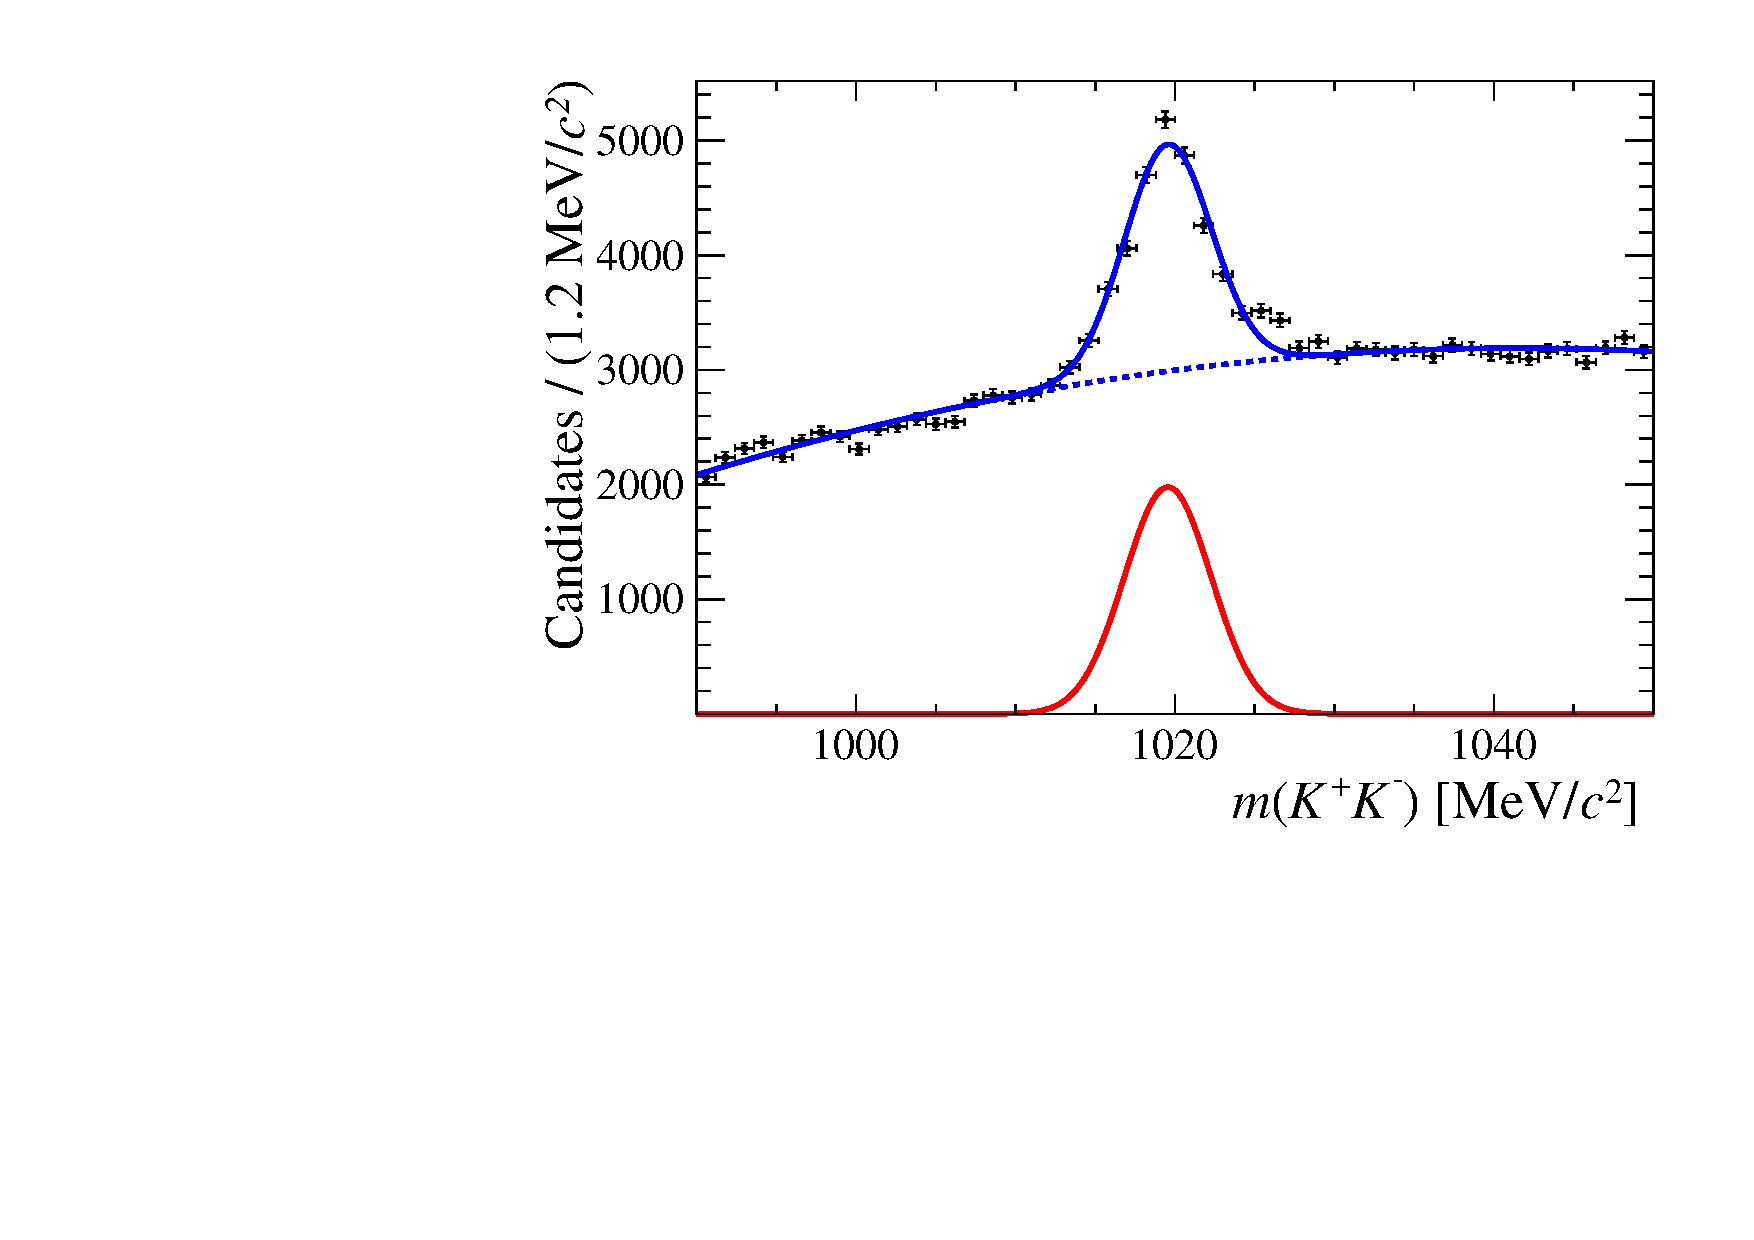
\includegraphics[width=1.0\textwidth]{figs/Selection/Fit_Data_Bs2JpsiPhi_Jpsi2MuMu_Phi2KK_2016_MagDown.pdf}
      \caption{\decay{\phiz}{\Kp\Km} MagDown}
   \end{subfigure}
   \begin{subfigure}[t]{0.4\textwidth}
      \centering
      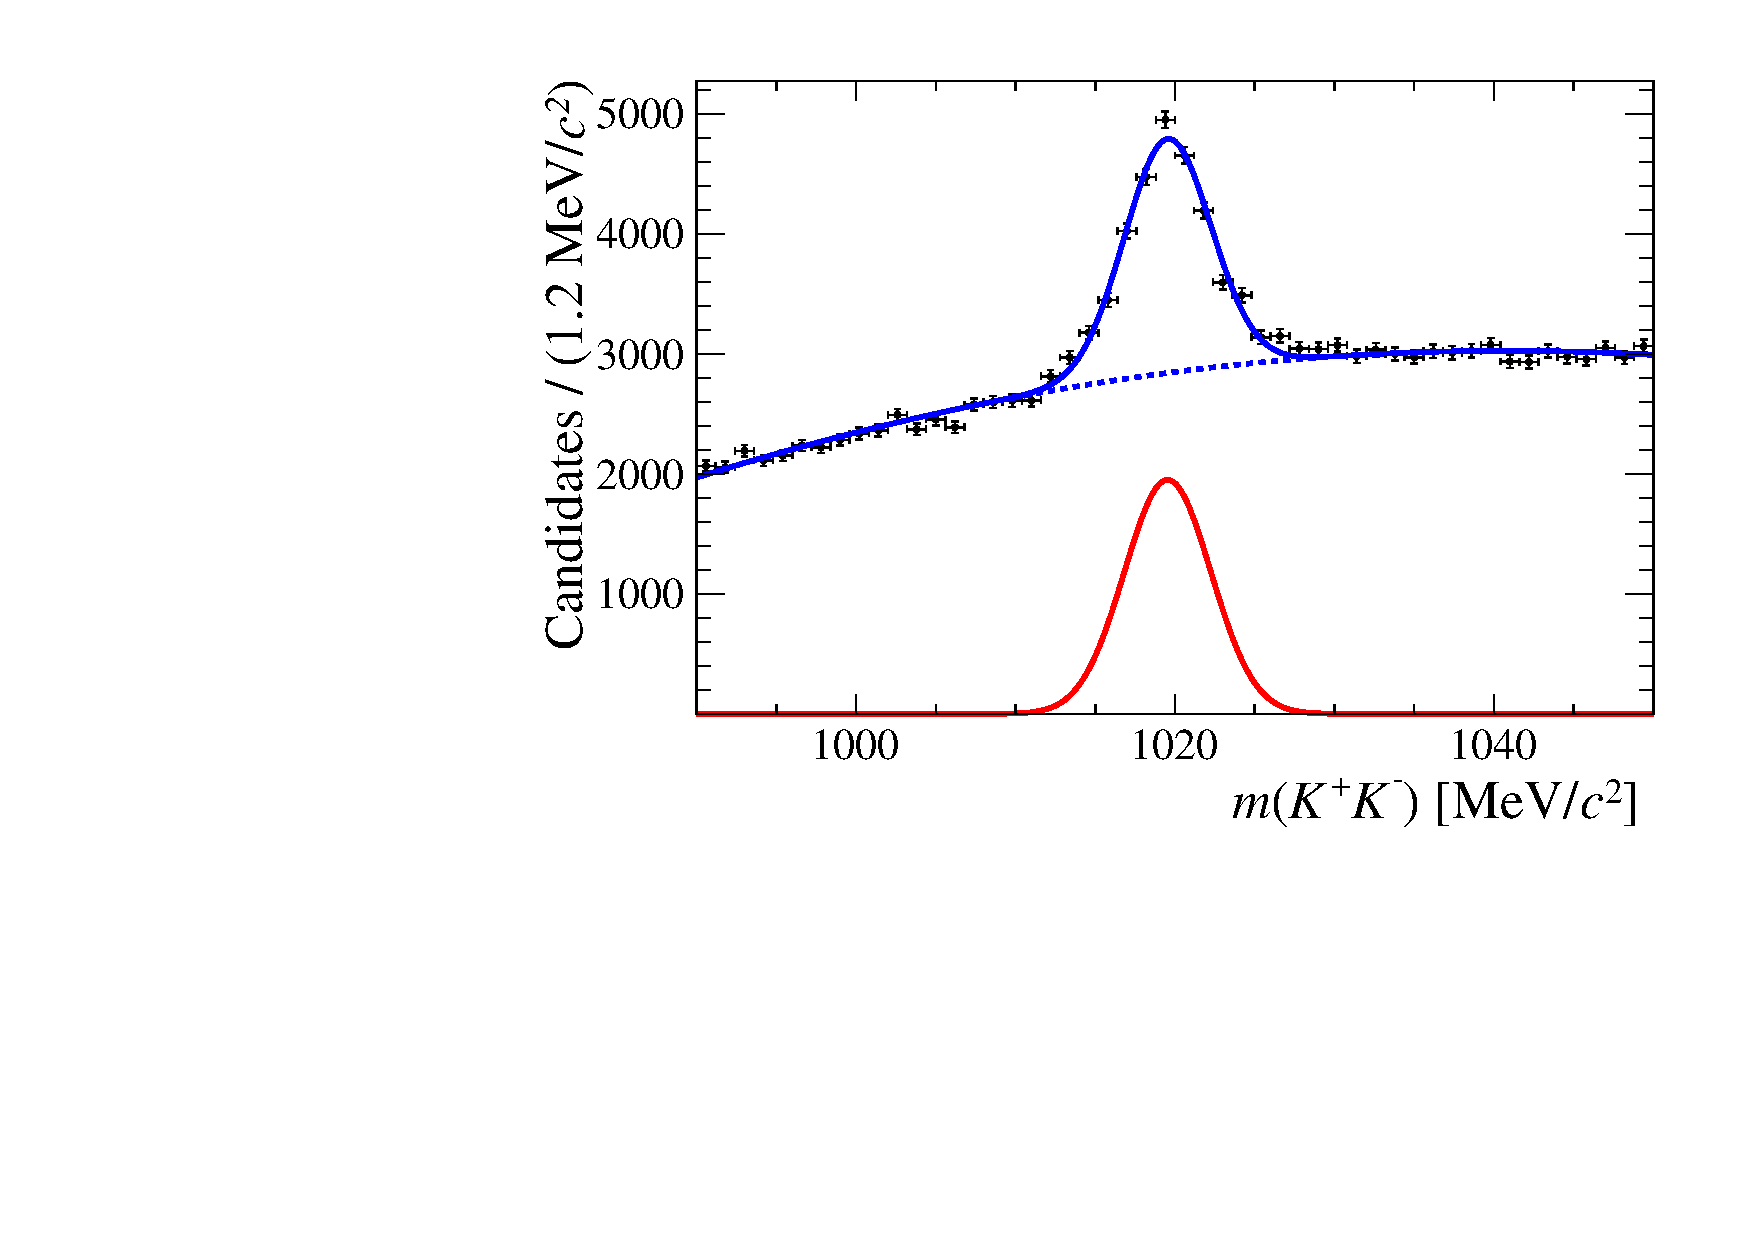
\includegraphics[width=1.0\textwidth]{figs/Selection/Fit_Data_Bs2JpsiPhi_Jpsi2MuMu_Phi2KK_2016_MagUp.pdf}
      \caption{\decay{\phiz}{\Kp\Km} MagUp}
   \end{subfigure}\\
   \begin{subfigure}[t]{0.4\textwidth}
      \centering
      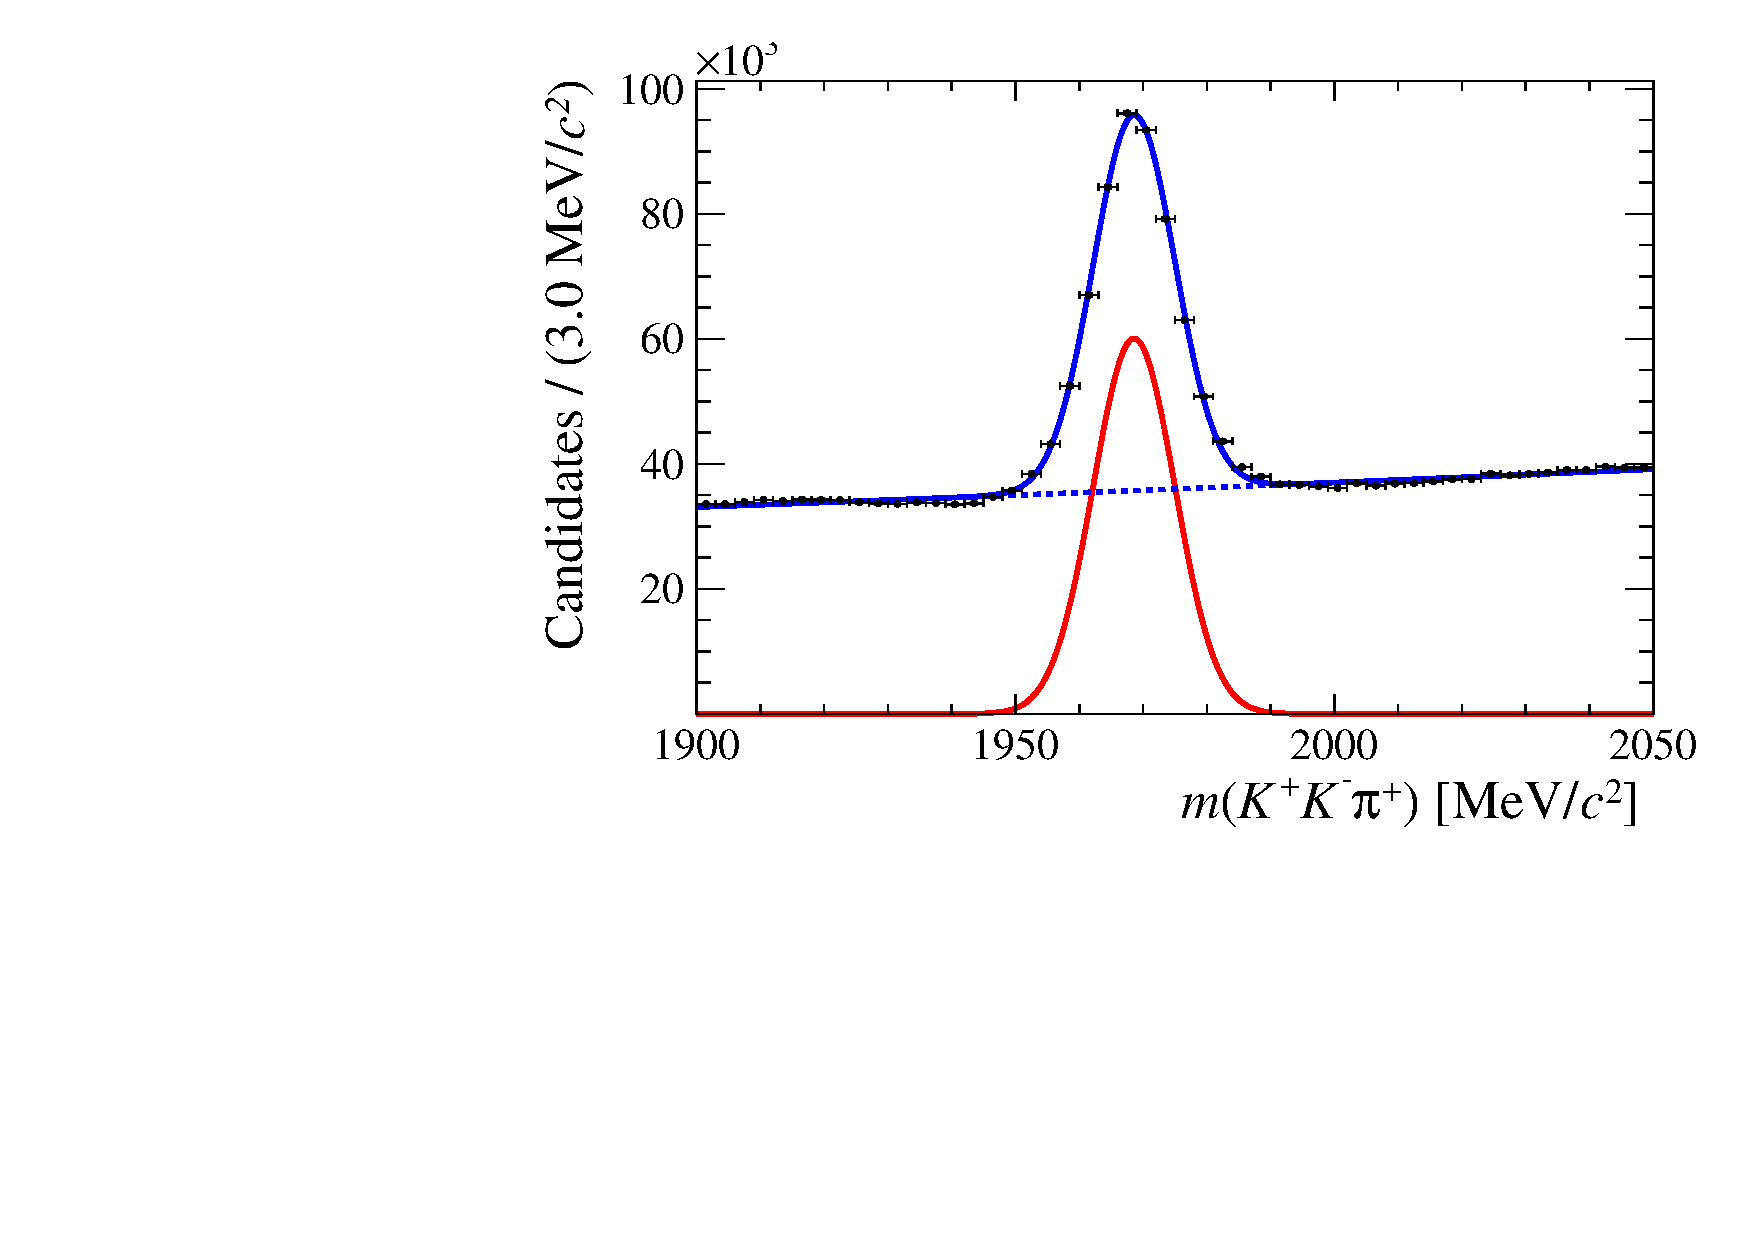
\includegraphics[width=1.0\textwidth]{figs/Selection/Fit_Data_Bs02DsPi_Ds2KKPi_2016_MagDown_PreSel.pdf}
      \caption{\decay{\Dsp}{\Kp\Km\pip} MagDown}
   \end{subfigure}
   \begin{subfigure}[t]{0.4\textwidth}
      \centering
      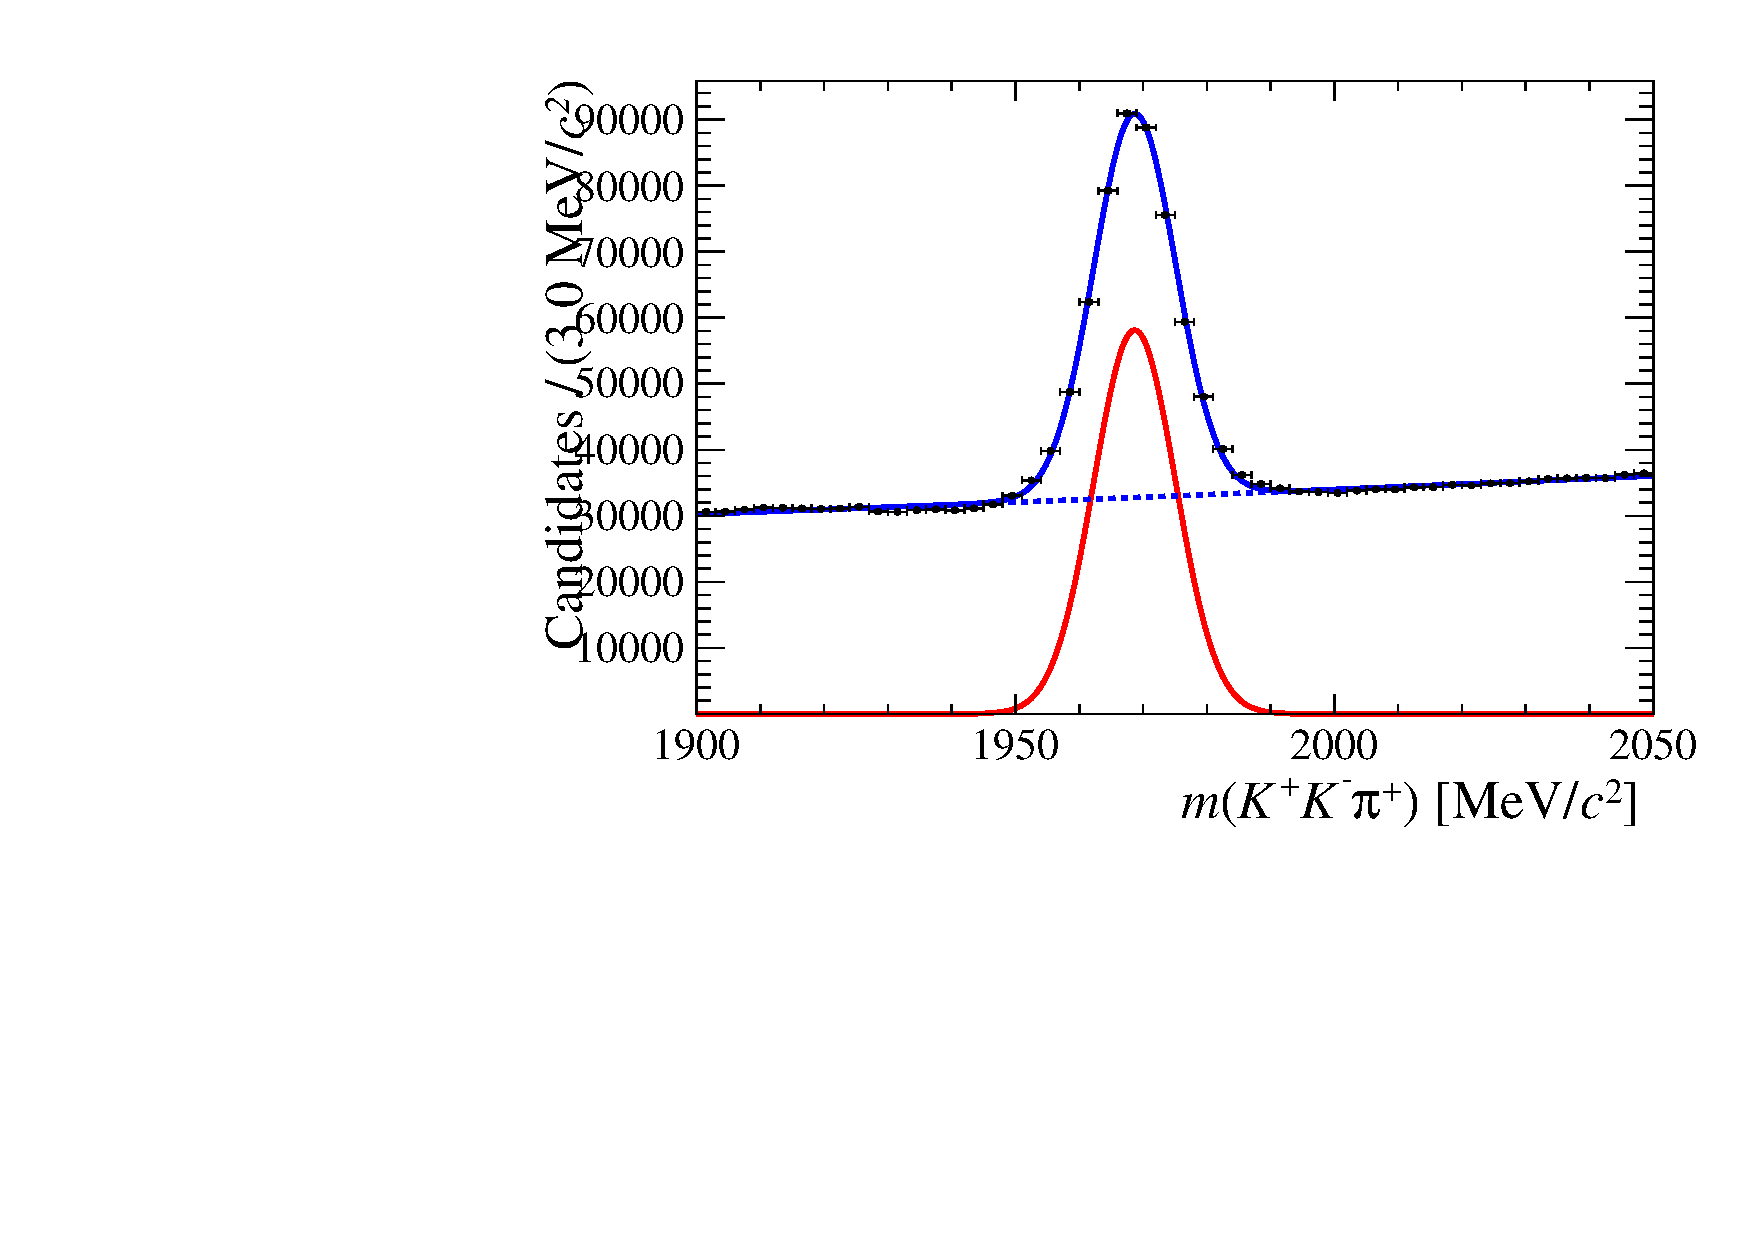
\includegraphics[width=1.0\textwidth]{figs/Selection/Fit_Data_Bs02DsPi_Ds2KKPi_2016_MagUp_PreSel.pdf}
      \caption{\decay{\Dsp}{\Kp\Km\pip} MagUp}
   \end{subfigure}
   \begin{subfigure}[t]{0.4\textwidth}
      \centering
      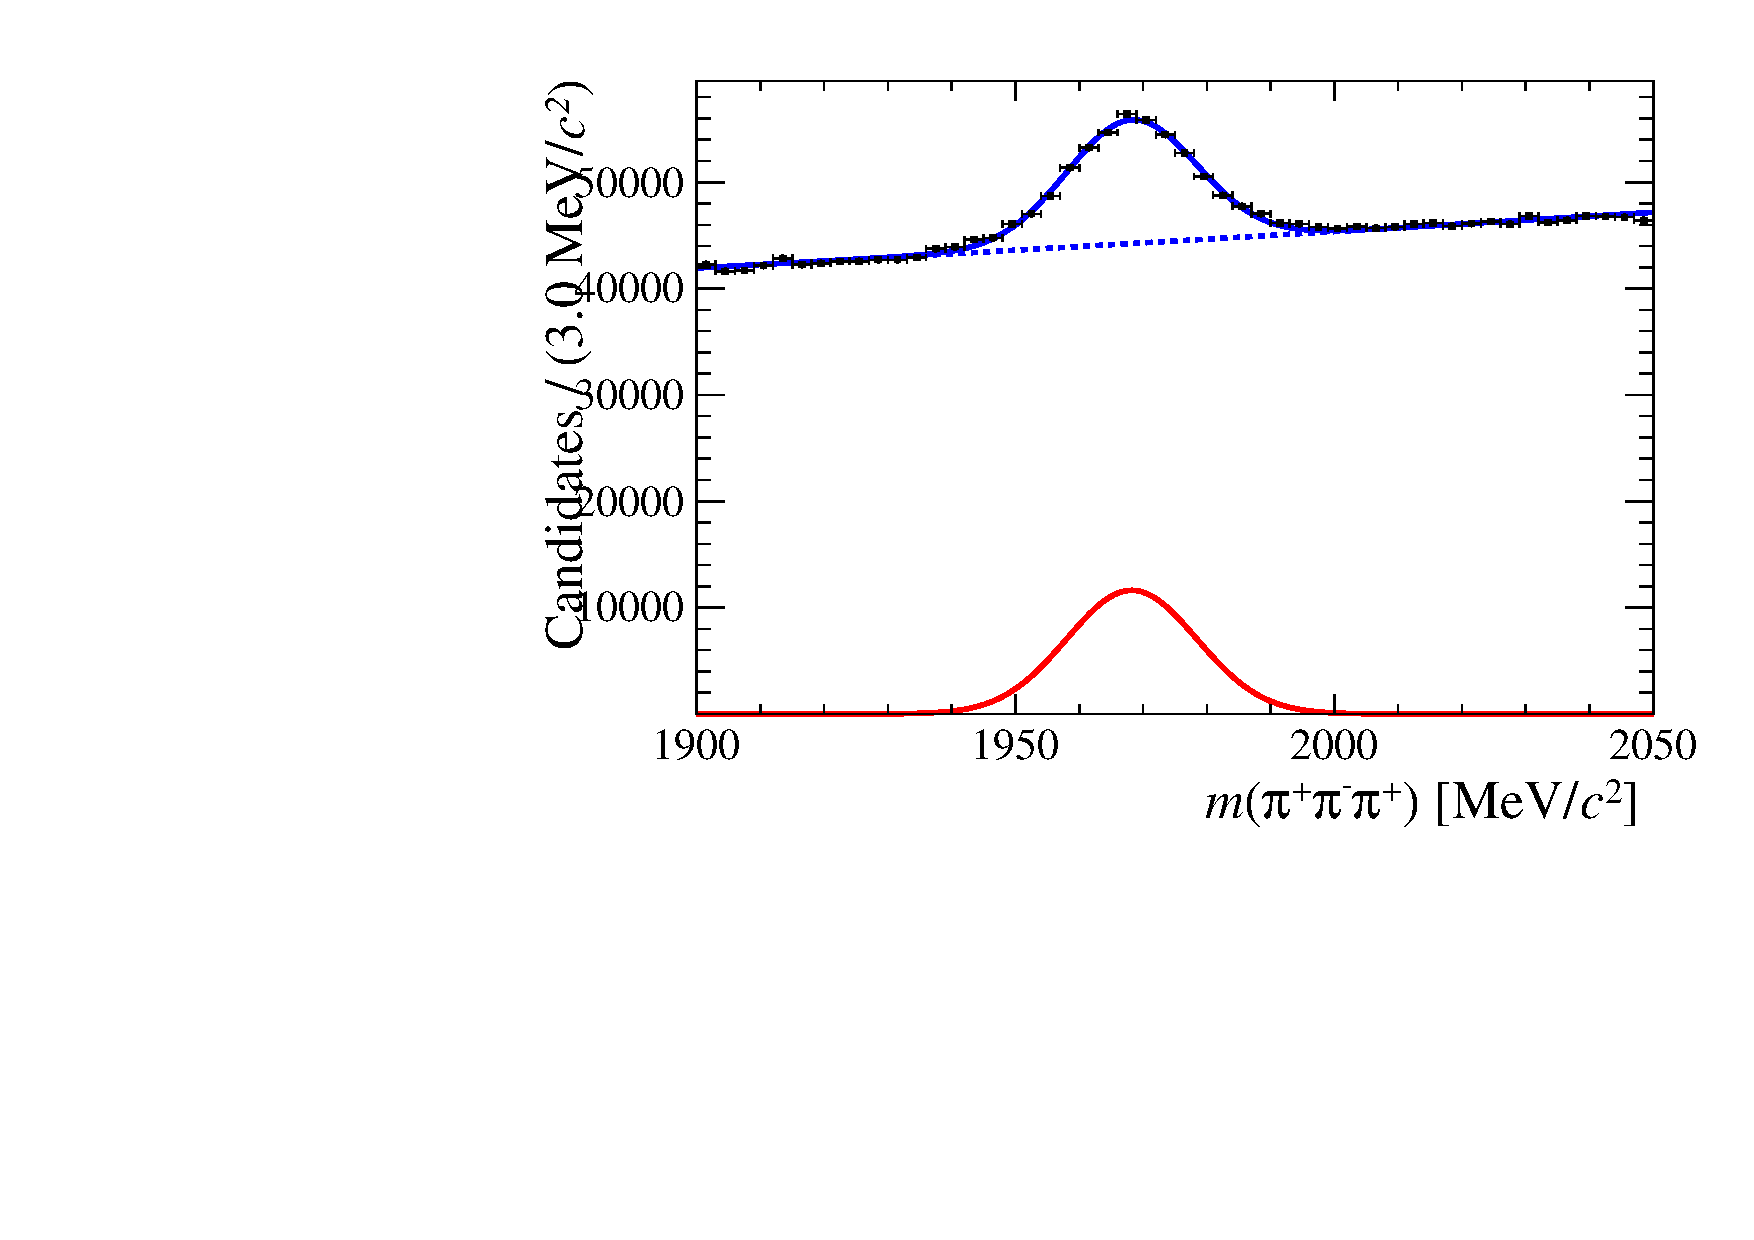
\includegraphics[width=1.0\textwidth]{figs/Selection/Fit_Data_Bs02DsPi_Ds2PiPiPi_2016_MagDown_PreSel.pdf}
      \caption{\decay{\Dsp}{\pip\pim\pip} MagDown}
   \end{subfigure}
   \begin{subfigure}[t]{0.4\textwidth}
      \centering
      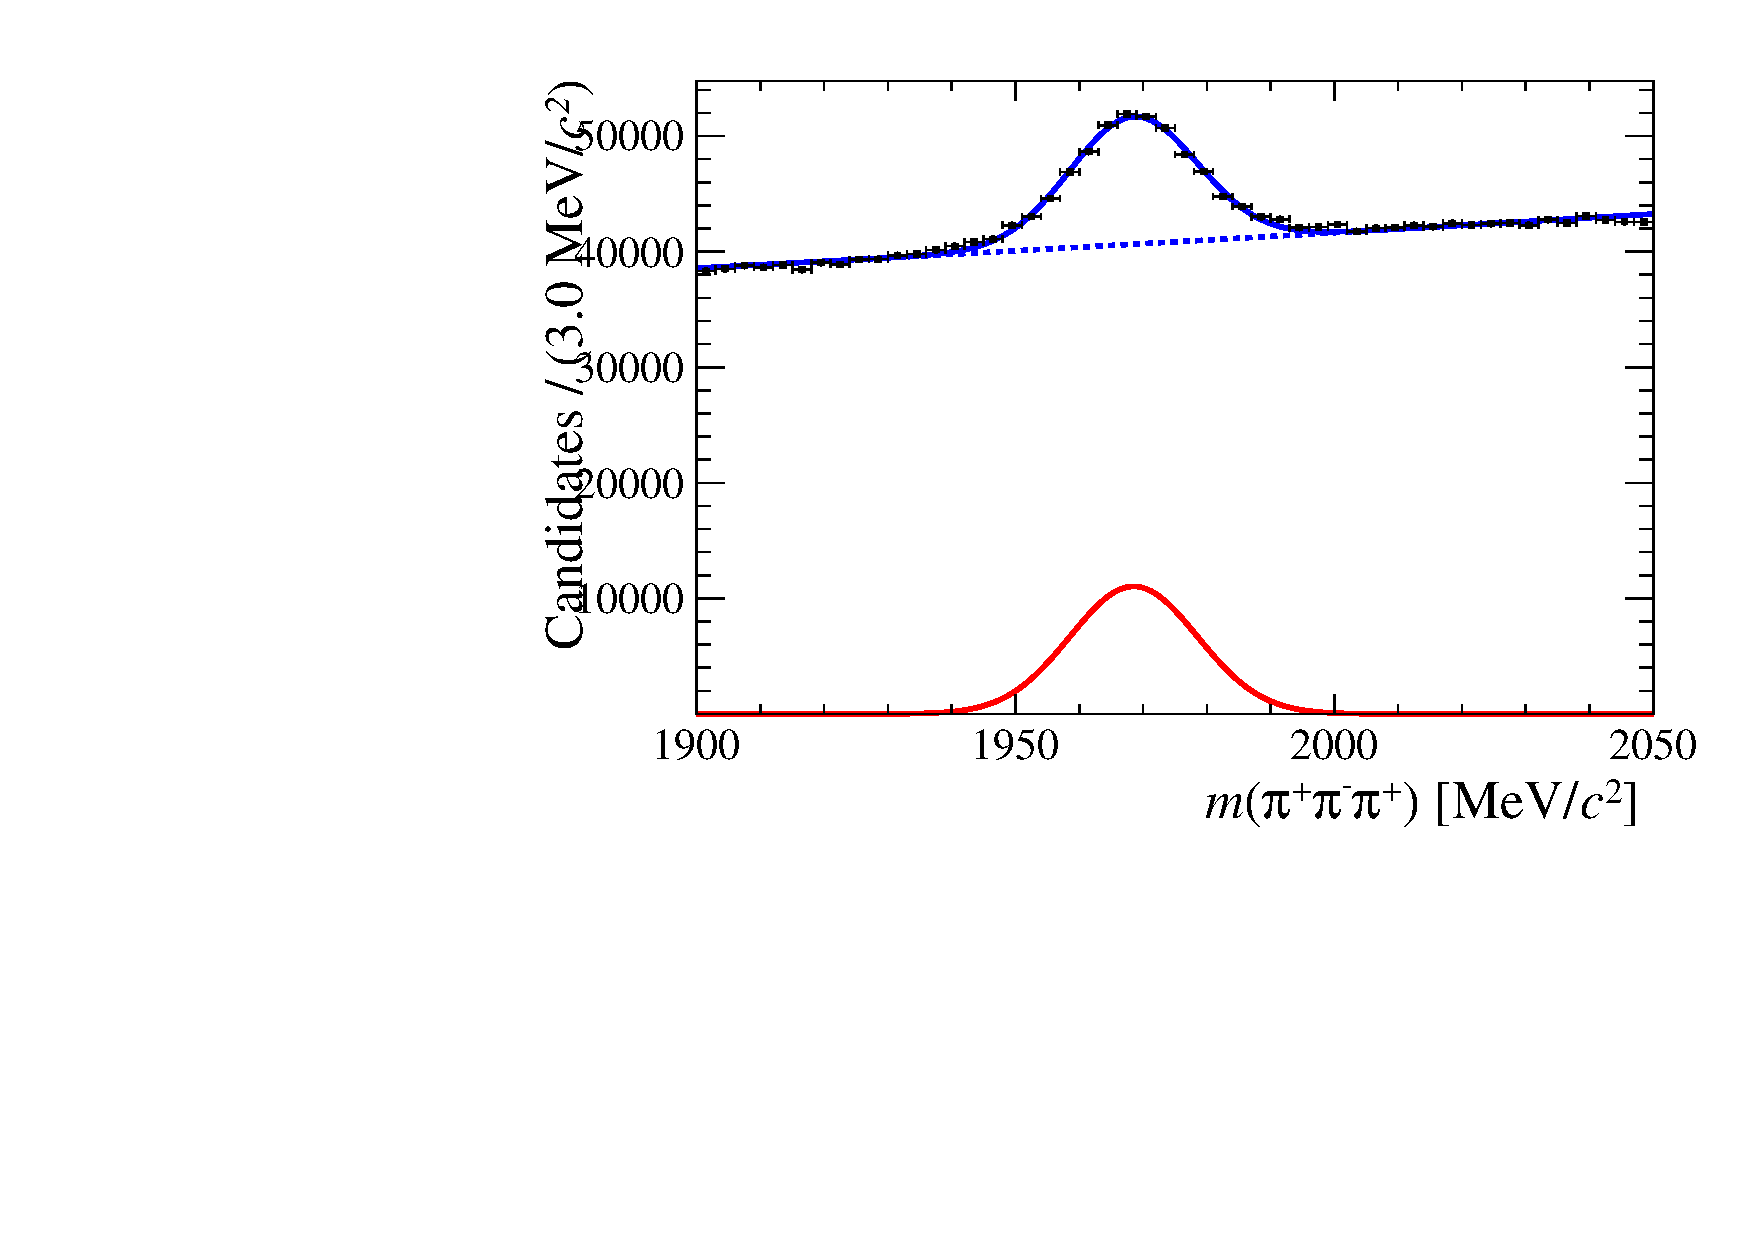
\includegraphics[width=1.0\textwidth]{figs/Selection/Fit_Data_Bs02DsPi_Ds2PiPiPi_2016_MagUp_PreSel.pdf}
      \caption{\decay{\Dsp}{\pip\pim\pip} MagUp}
   \end{subfigure}
   \begin{subfigure}[t]{0.4\textwidth}
      \centering
      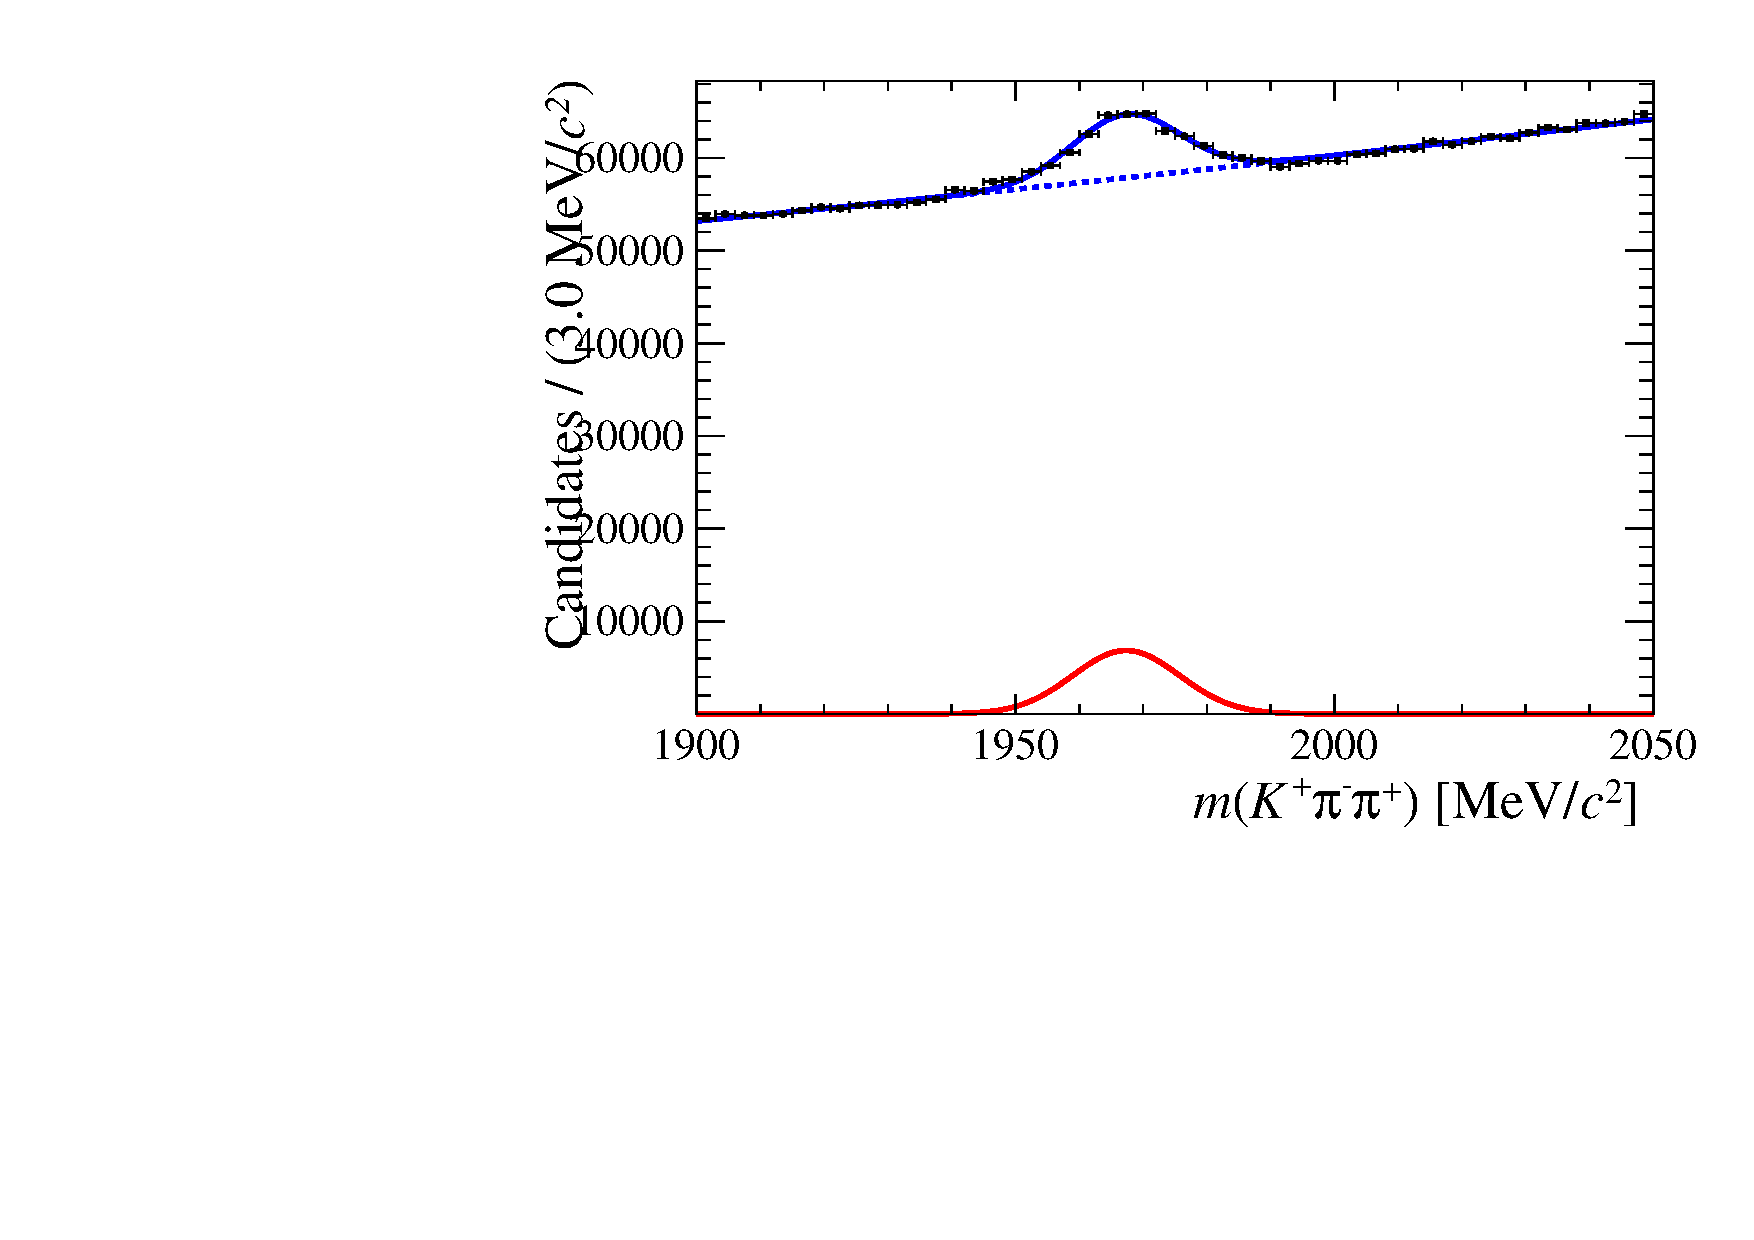
\includegraphics[width=1.0\textwidth]{figs/Selection/Fit_Data_Bs02DsPi_Ds2KPiPi_2016_MagDown_PreSel.pdf}
      \caption{\decay{\Dsp}{\Kp\pim\pip} MagDown}
   \end{subfigure}
   \begin{subfigure}[t]{0.4\textwidth}
      \centering
      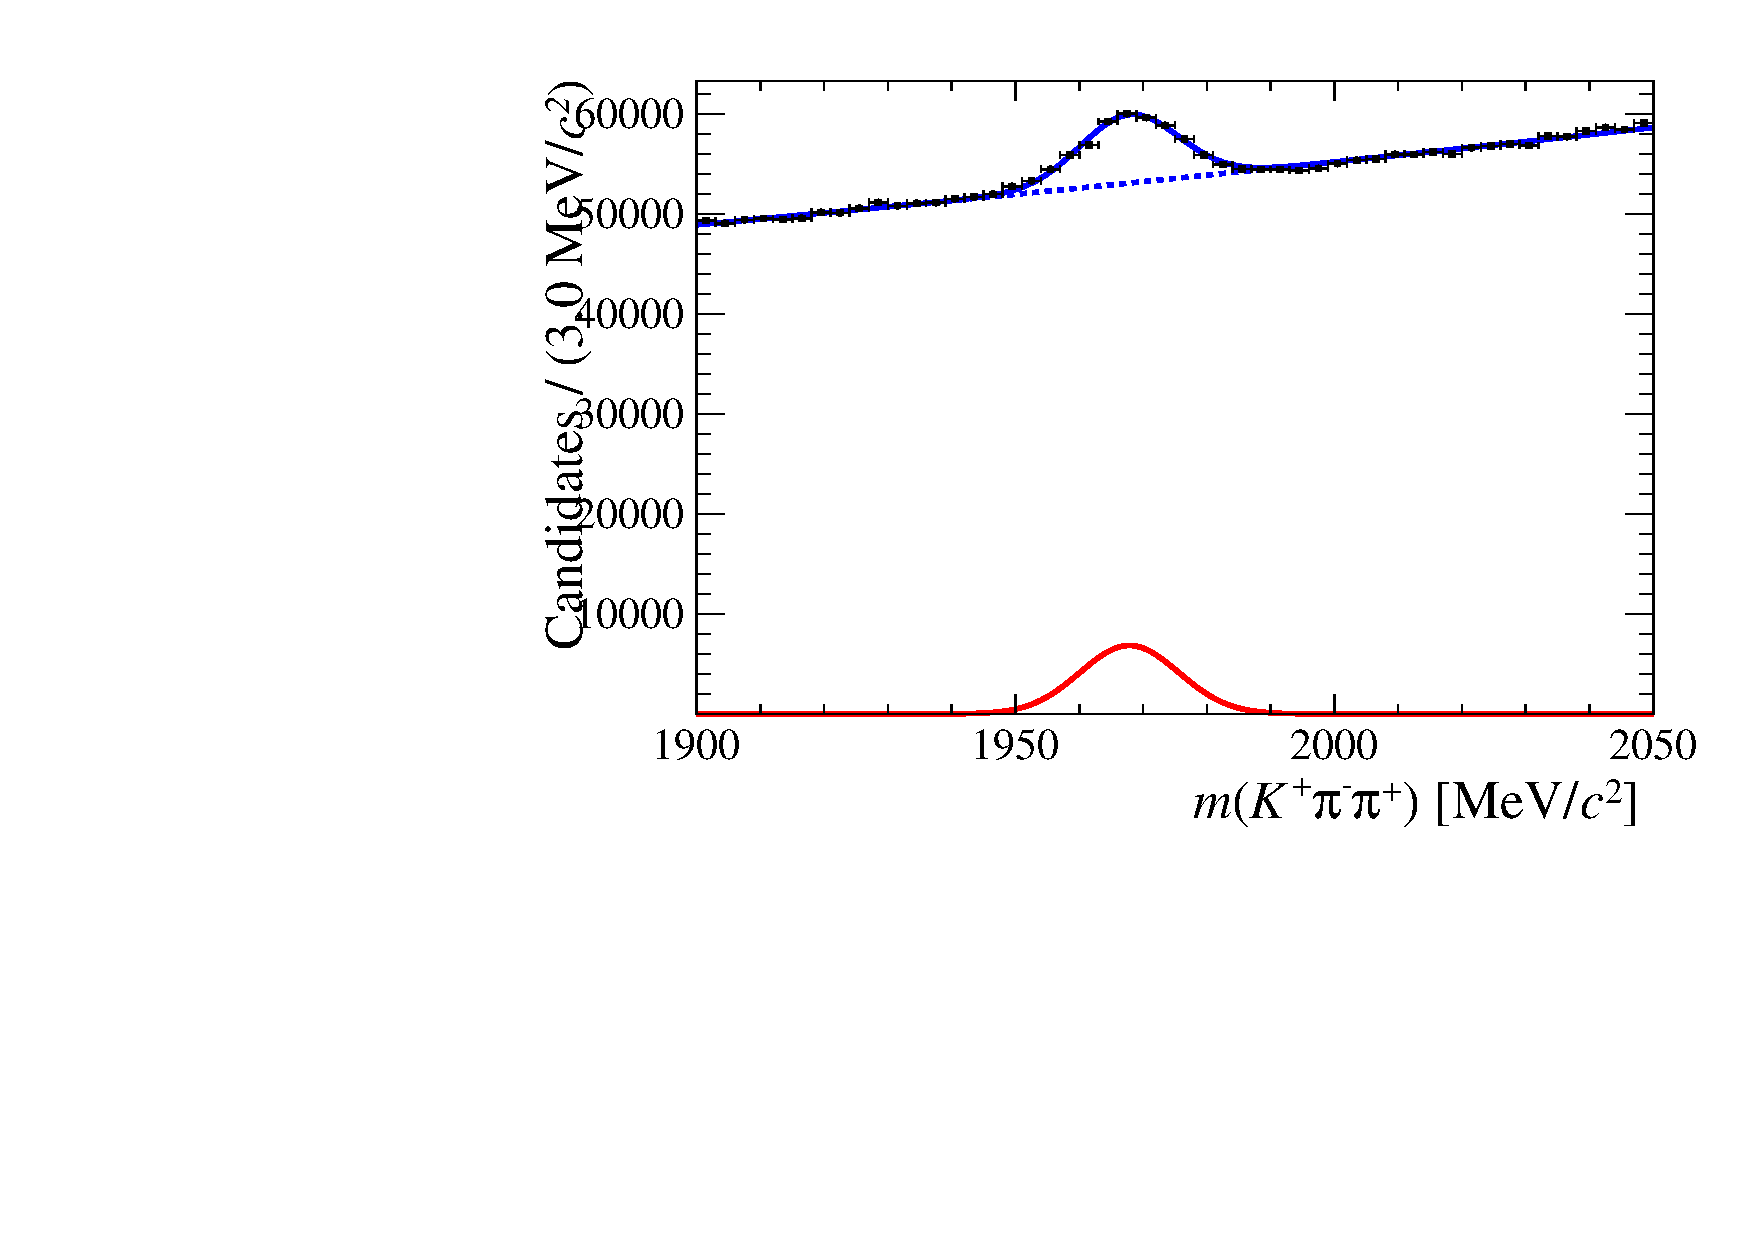
\includegraphics[width=1.0\textwidth]{figs/Selection/Fit_Data_Bs02DsPi_Ds2KPiPi_2016_MagUp_PreSel.pdf}
      \caption{\decay{\Dsp}{\Kp\pim\pip} MagUp}
   \end{subfigure}
   \caption{Unbinned maximum likelihood fit to \decay{\Bs}{\jpsi\phiz} (top) and \decay{\Bsb}{\Dsp\pim} (bottom three rows) candidates. These distributions correspond to just the 2016 data samples. Slight discrepancies are observed as a result of the simplified fit model in the top two plots.}
   \label{fig:mvatrainingsamples}
\end{figure}


%%%%%%%%%%%%%%%%%%%%%%%%%%%%%%%%%%%%%%%%%%%%%%%%%%%%%%%%%%
\begin{table}[!h]
   \centering
      \begin{tabular}{ll S[table-format=6.0(4)] S[table-format=6.0(4)] S[table-format=7.0(4)]}
         \hline
         Mode                       & Year   & {MagDown}          & {MagUp}           & {Total} \\ 
         \hline                                                
         \decay{\phiz}{\Kp\Km}      & 2011   & 3190 \pm 170     &   2120 \pm 140  &    \\
                                    & 2012   & 5800 \pm 200     &   5540 \pm 200  &     \\
                                    & 2015   & 2240 \pm 110     &   1640 \pm 100  &     \\
                                    & 2016   & 11200 \pm 300    &   11100 \pm 300 & 42830 \pm 600    \\
         \hline                                                
         \decay{\Dsp}{\Kp\Km\pip}   & 2011   & 97100  \pm 500   & 68600  \pm 400  &     \\
                                    & 2012   & 216600 \pm 800   & 212800 \pm 800  &     \\
                                    & 2015   & 68600  \pm 400   & 43400  \pm 300  &     \\
                                    & 2016   & 321400 \pm 900   & 310800 \pm 900  & 1339300 \pm 1900    \\
         \hline                                                
         \decay{\Dsp}{\pip\pim\pip} & 2011   & 24300 \pm 500    &   17100 \pm 400 &      \\
                                    & 2012   & 57700 \pm 800    &   56500 \pm 900 &     \\
                                    & 2015   & 20400 \pm 500    &   13100 \pm 400 &     \\
                                    & 2016   & 99200 \pm 1200   &  92100 \pm 1200 & 380400 \pm 2300    \\
         \hline                                                
         \decay{\Dsp}{\Kp\pim\pip}  & 2011   & 13200 \pm 600    & 9500  \pm 400   &     \\
                                    & 2012   & 29300 \pm 900    & 29300 \pm 900   &     \\
                                    & 2015   & 10000 \pm 500    & 6200  \pm 400   &     \\
                                    & 2016   & 47800 \pm 1200   & 44200 \pm 1100  & 189500 \pm 2300    \\
         \hline
      \end{tabular}
      \caption{Yields of the samples used to train data-driven MVAs. The total yields are summed over all years and both magnet polarities.}
      \label{table:mva_training_yields}
   
\end{table}
%%%%%%%%%%%%%%%%%%%%%%%%%%%%%%%%%%%%%%%%%%%%%%%%%%%%%%%%%%

\section{Input variables}
\label{sec:App_MVA_input}

Examples of the MVA input variable ranking are shown for the Run~II, \decay{\phiz}{\Kp\Km} MVA and Run~II, \decay{\Dsp}{\Kp\Km\pip} MVA in Table~\ref{tab:mvarank_dsandphi}. It can be seen that for both the \Dsp and \phiz meson MVAs that the kaon particle identification variable and various $\log_{10}(\chi^{2}_{\text{IP}})$ variables are the most discriminating.

\begin{table}[h]
\centering
\scalebox{1.0}{
\begin{tabular}{ c l c | c l c}

\hline 

\multicolumn{3}{c|}{\decay{\Dsp}{\Kp\Km\pip}}                 & \multicolumn{3}{c}{\decay{\phiz}{\Kp\Km}}                       \\
Rank & Variable                             & Importance (\%) & Rank & Variable                           & Importance (\%)      \\
\hline
 1 & \Kp ProbNNk                            & $7.6$ &  1 & \Kp ProbNNk                                & $6.0$\\
 2 & \Km ProbNNk                            & $6.0$ &  2 & \phiz $\log_{10}(\chi^{2}_{\text{IP}})$    & $6.0$\\
 3 & \Kp $\log_{10}(\chi^{2}_{\text{IP}})$  & $5.5$ &  3 & \Km $\log_{10}(\chi^{2}_{\text{IP}})$      & $6.0$\\
 4 & \pip $\log_{10}(\chi^{2}_{\text{IP}})$ & $5.0$ &  4 & \phiz $\log_{10}(\chi^{2}_{\text{VTX}})$   & $5.8$\\
 5 & \Kp \ptot                              & $4.3$ &  5 & \Km ProbNNpi                               & $5.8$\\
 6 & \Dsp $\log_{10}(\chi^{2}_{\text{IP}})$ & $4.1$ &  6 & \Kp $\log_{10}(\chi^{2}_{\text{IP}})$      & $5.8$\\
 7 & \pip \pt                               & $4.0$ &  7 & \Kp ProbNNghost                            & $5.4$\\
 8 & \Kp \pt                                & $3.9$ &  8 & \Km ProbNNk                                & $5.4$\\
 9 & \pip ProbNNpi                          & $3.9$ &  9 & \Kp $\chi^{2}_{\text{TRK}}$                & $5.6$\\
10 & \Dsp $\log_{10}(\chi^{2}_{\text{FD}})$ & $3.8$ & 10 & \Km $\chi^{2}_{\text{TRK}}$                & $5.2$\\
11 & \Km $\log_{10}(\chi^{2}_{\text{IP}})$  & $3.7$ & 11 & \Kp ProbNNpi                               & $5.2$\\
12 & \Dsp $\log_{10}(\chi^{2}_{\text{VTX}})$& $3.0$ & 12 & \Km ProbNNghost                            & $5.0$\\
13 & \Km \ptot                              & $2.8$ & 13 & \Kp ProbNNp                                & $4.5$\\
14 & \Kp ProbNNp                            & $2.8$ & 14 & \Km ProbNNp                                & $4.4$\\
15 & \Km ProbNNp                            & $2.7$ & 15 & \Kp $\chi^{2}_{\text{TRKMATCH}}$           & $4.3$\\
% 16 & \pip ProbNNghost                   & $2.623$ & 16 & \Km $\chi^{2}_{\text{TRKMATCH}}$     & $3.977\times 10^{-2}$\\
% 17 & \Kp ProbNNghost                    & $2.593$ & 17 & \Km \pt                              & $3.437\times 10^{-2}$\\
% 18 & \Dsp \pt                           & $2.543$ & 18 & \Kp \pt                              & $3.012\times 10^{-2}$\\
% 19 & \Kp ProbNNpi                       & $2.525$ & 19 & \phiz PT                             & $2.400\times 10^{-2}$\\
% 20 & \Km \pt                            & $2.355$ & 20 & \phiz P                              & $1.792\times 10^{-2}$\\
% 21 & \Dsp \ptot                         & $2.327$ & 21 & \Km \pz                              & $1.397\times 10^{-2}$\\
% 22 & \Km ProbNNpi                       & $2.226$ & 22 & \Km \ptot                            & $1.387\times 10^{-2}$\\
% 23 & \pip \ptot                         & $2.083$ & 23 & \Kp \pz                              & $1.245\times 10^{-2}$\\
% 24 & \pip ProbNNp                       & $1.849$ & 24 & \Kp \ptot                            & $1.218\times 10^{-2}$\\
% 25 & \pip ProbNNk                       & $1.793$ \\
% 26 & \Km ProbNNghost                    & $1.607$ \\
% 27 & \pip $\chi^{2}_{\text{TRKVELO}}$   & $1.589$ \\
% 28 & \Km $\chi^{2}_{\text{TRK}}$        & $1.588$ \\
% 29 & \pip $\chi^{2}_{\text{TRKMATCH}}$  & $1.548$ \\
% 30 & \Kp $\chi^{2}_{\text{TRK}}$        & $1.522$ \\
% 31 & \Km $\chi^{2}_{\text{TRKMATCH}}$   & $1.442$ \\
% 32 & \pip $\chi^{2}_{\text{TRK}}$       & $1.433$ \\
% 33 & \Kp $\chi^{2}_{\text{TRKVELO}}$    & $1.184$ \\
% 34 & \Kp $\chi^{2}_{\text{TRKMATCH}}$   & $1.176$ \\
% 35 & \Km $\chi^{2}_{\text{TRKVELO}}$    & $8.818\times10^{-3}$ \\
\hline
\end{tabular}
}
\caption{Ranking of variables for the 15 highest ranked variables used to train the \decay{\Dsp}{\Kp\Km\pip} (left) and \decay{\phiz}{\Kp\Km} (right) Run~II MVAs.}
\label{tab:mvarank_dsandphi}
\end{table}

Examples of the MVA training variable distributions are shown in Fig.~\ref{fig:mvatrainingvariables_phi} and~\ref{fig:mvatrainingvariables_Ds}.
%%%%%%%%%%%%%%%%%%%%%%%%%%%%%%%%%%%%%%%%%%%%%%%%%%%%%%%%%%
\begin{figure}[!h]
   \centering
   \begin{subfigure}[t]{0.22\textwidth}
      \centering
      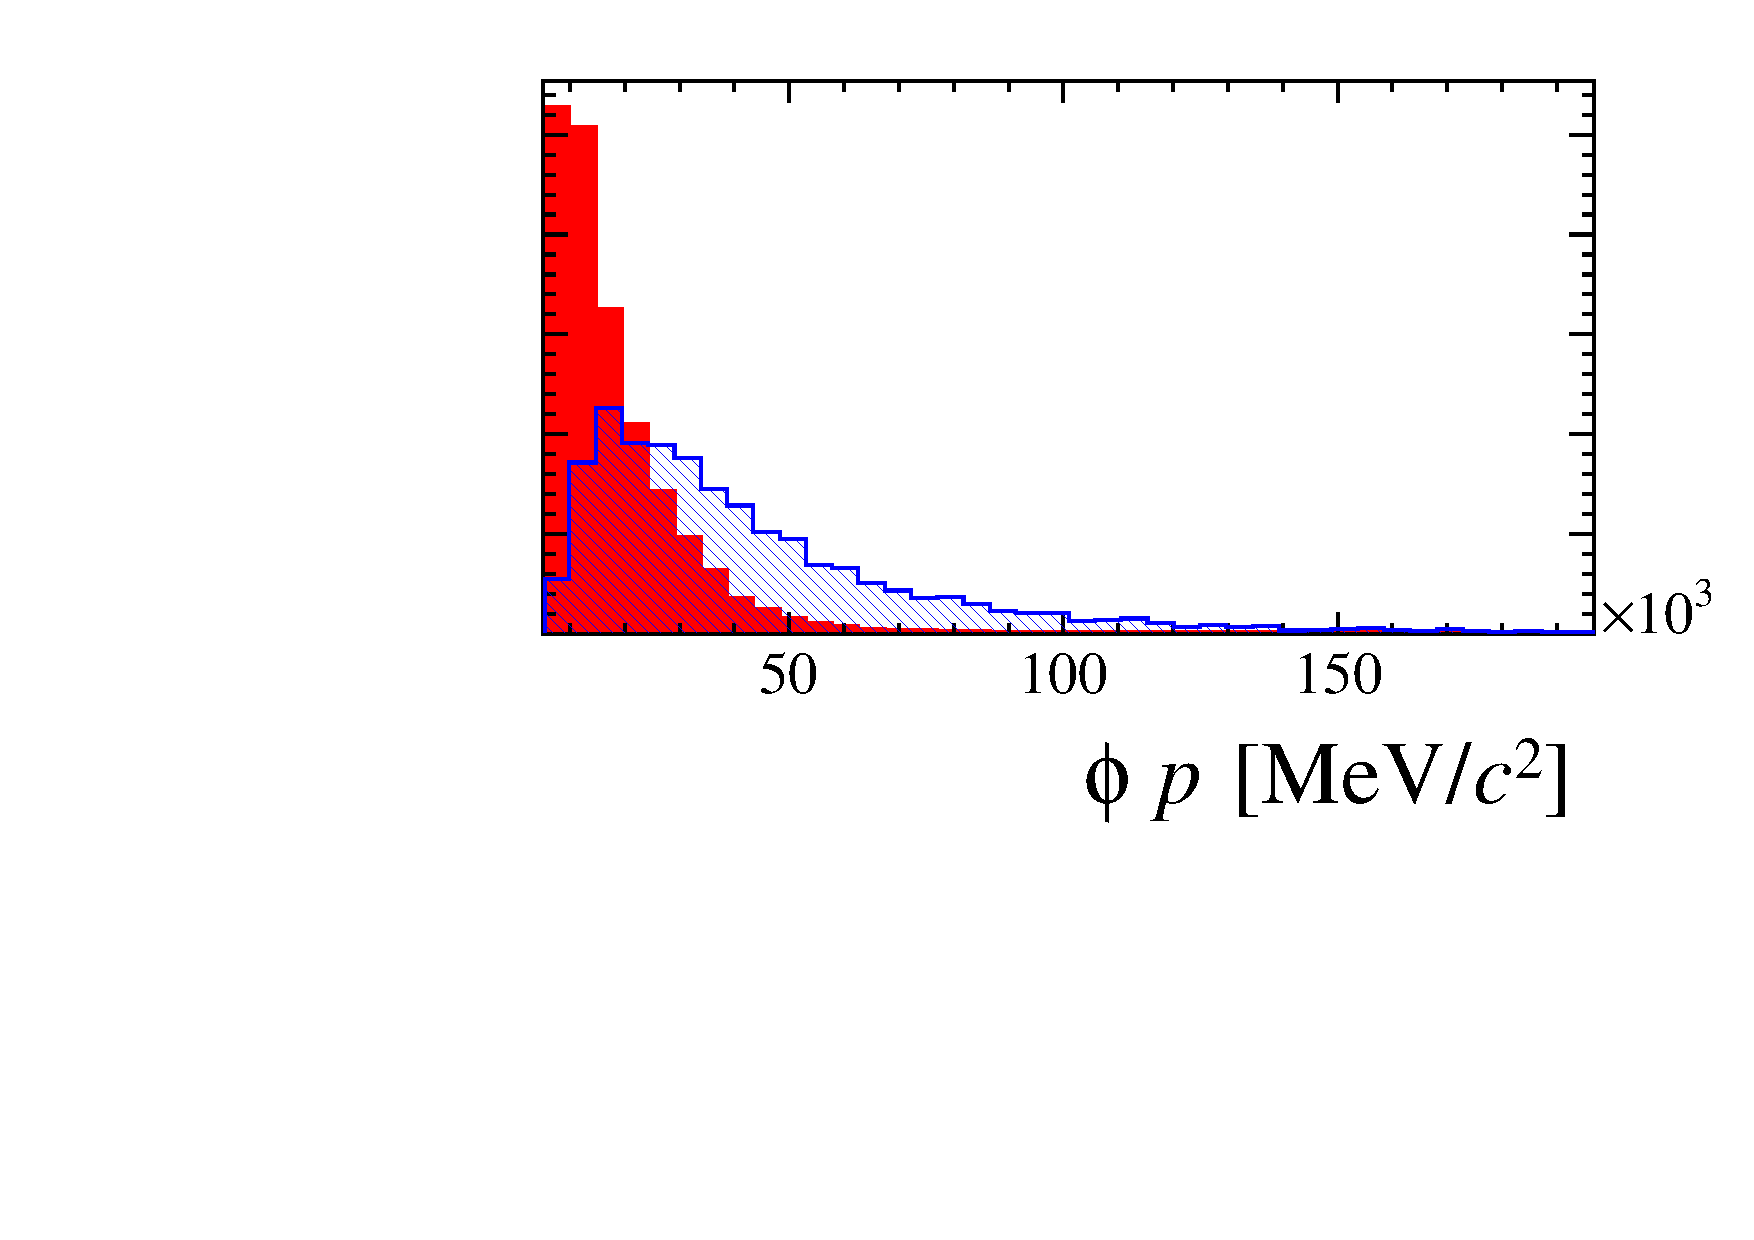
\includegraphics[width=1.0\textwidth]{figs/Selection/Phi_BDT_Var_Ds2KKPi_Phi_P.pdf}
   \end{subfigure}
   \begin{subfigure}[t]{0.22\textwidth}
      \centering
      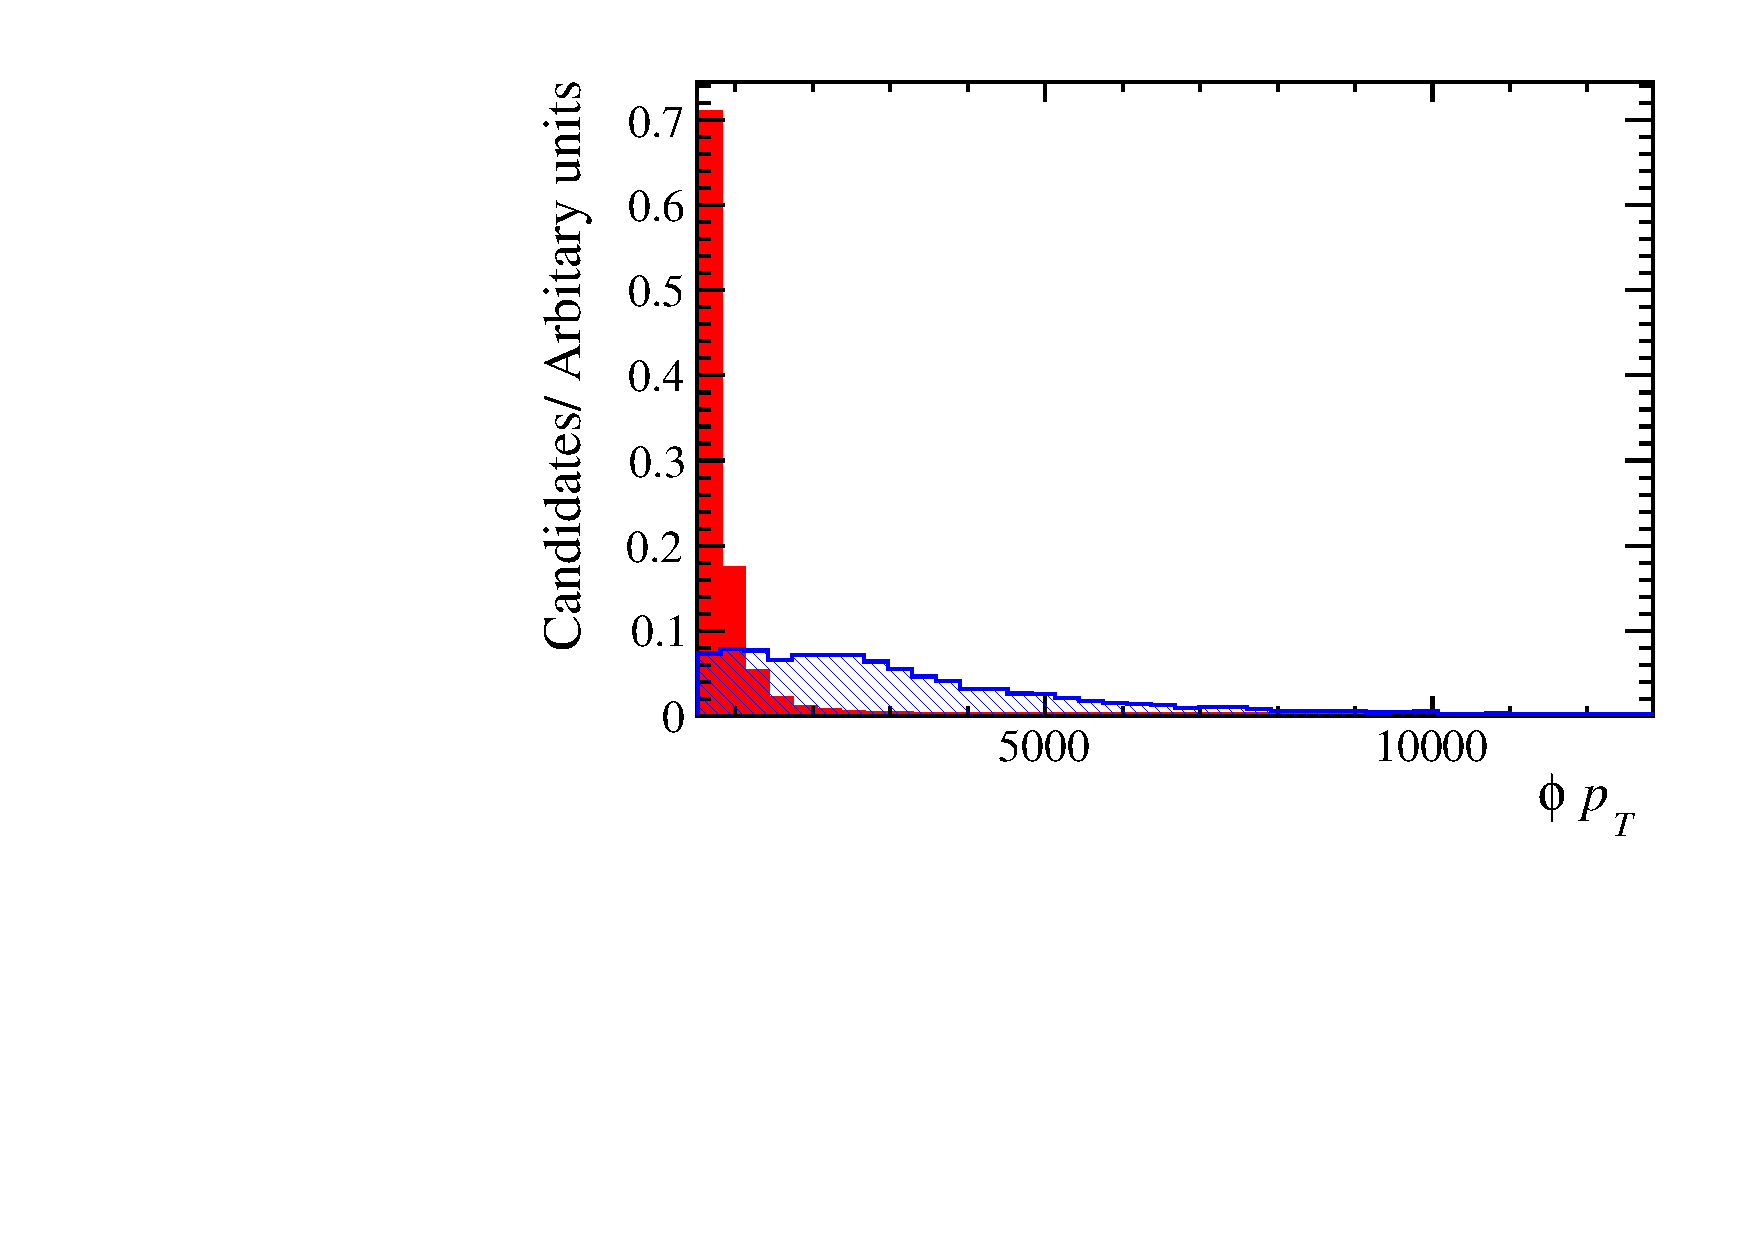
\includegraphics[width=1.0\textwidth]{figs/Selection/Phi_BDT_Var_Ds2KKPi_Phi_PT.pdf}
   \end{subfigure}
   \begin{subfigure}[t]{0.22\textwidth}
      \centering
      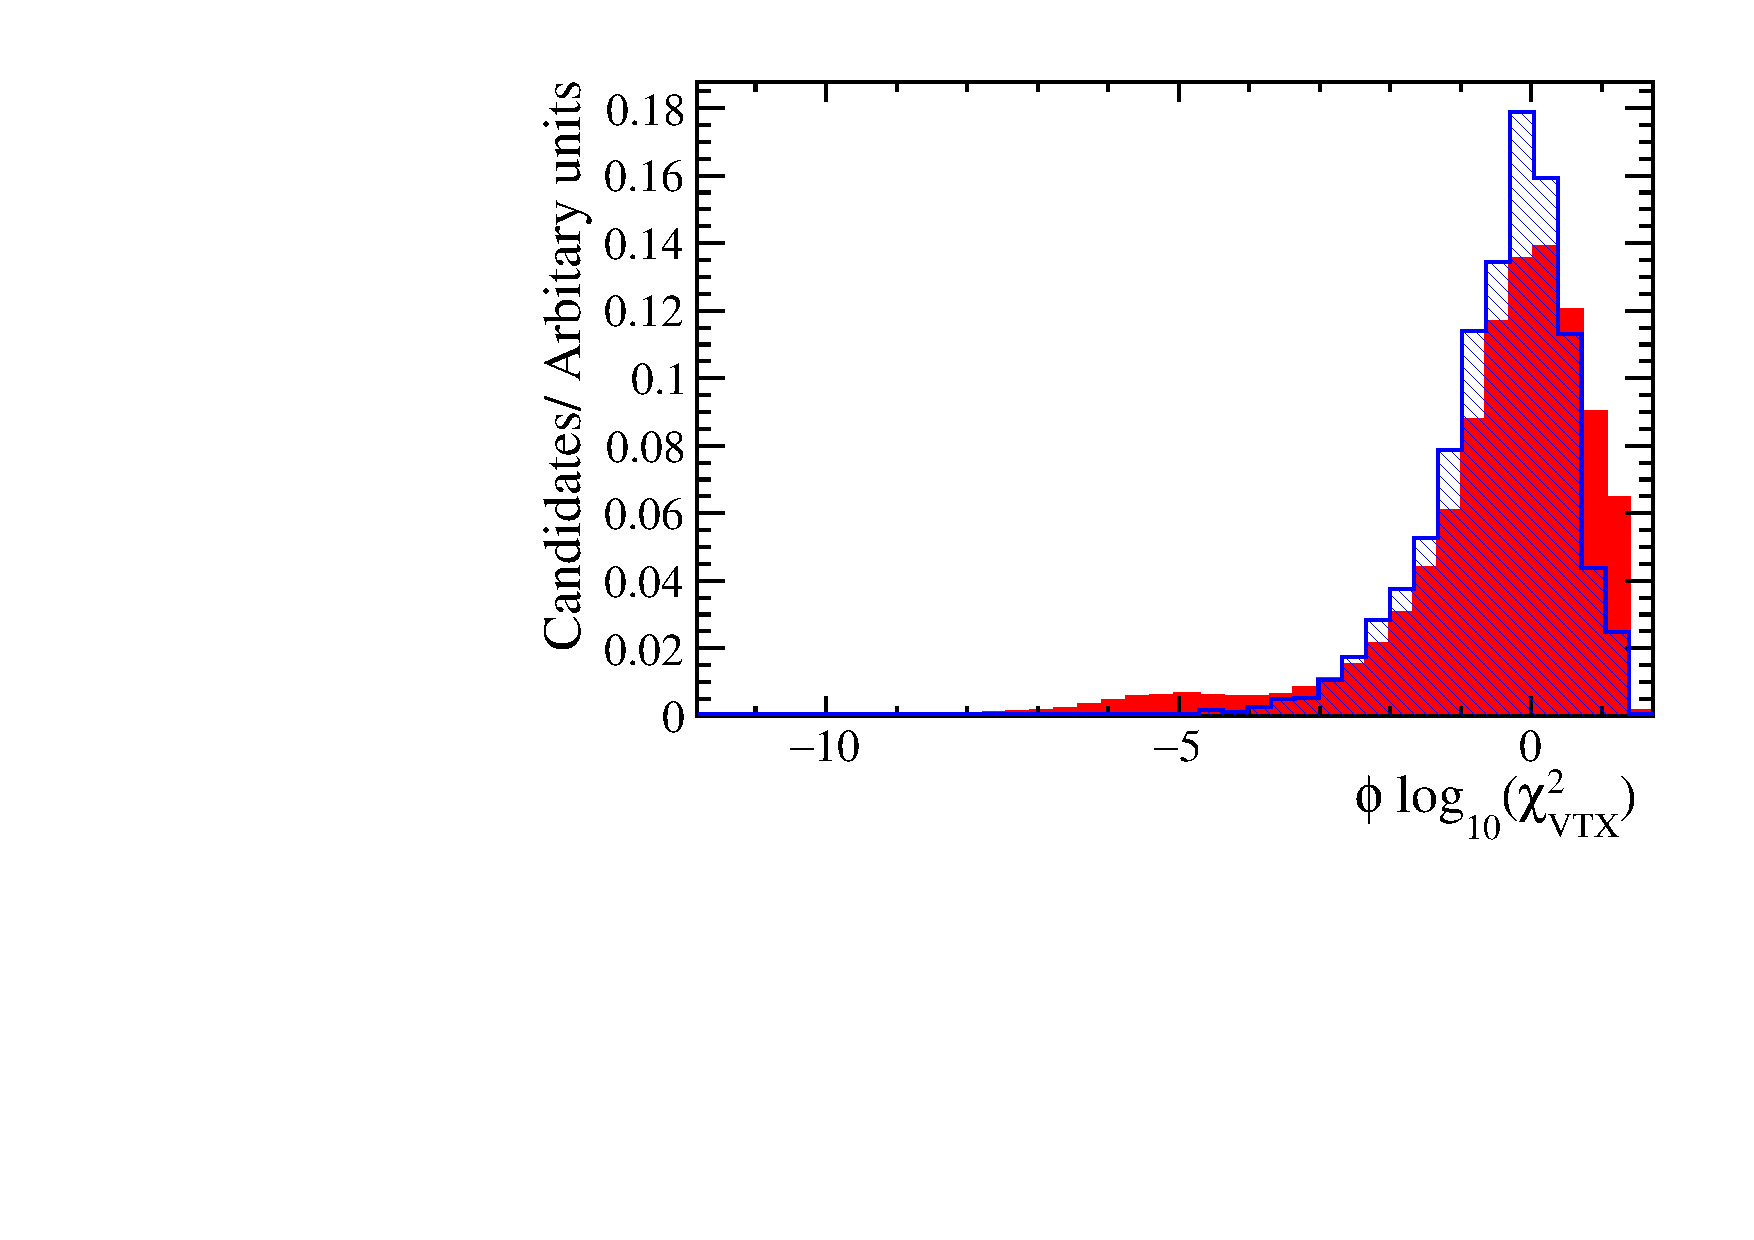
\includegraphics[width=1.0\textwidth]{figs/Selection/Phi_BDT_Var_Ds2KKPi_log10_Phi_ENDVERTEX_CHI2.pdf}
   \end{subfigure}
   \begin{subfigure}[t]{0.22\textwidth}
      \centering
      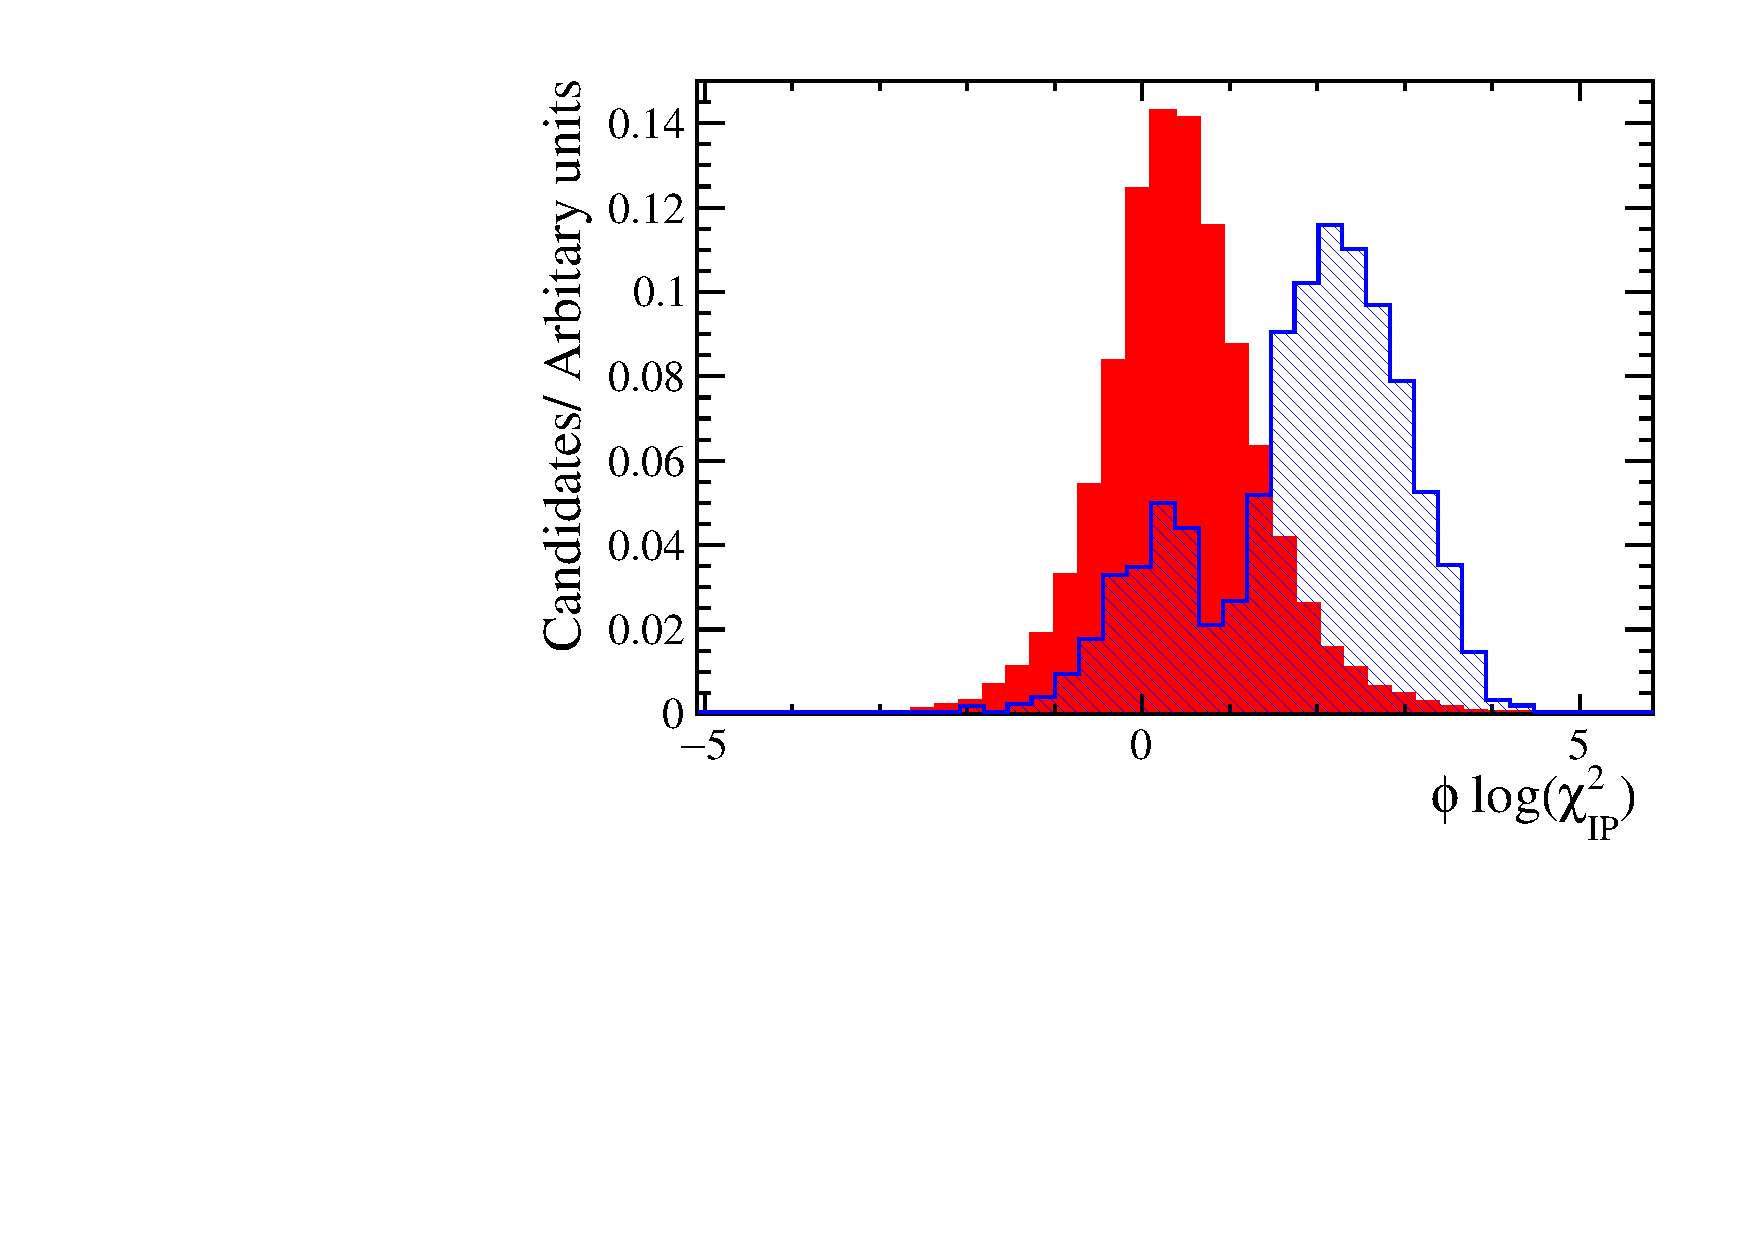
\includegraphics[width=1.0\textwidth]{figs/Selection/Phi_BDT_Var_Ds2KKPi_log10_Phi_IPCHI2_OWNPV.pdf}
   \end{subfigure}
   \begin{subfigure}[t]{0.22\textwidth}
      \centering
      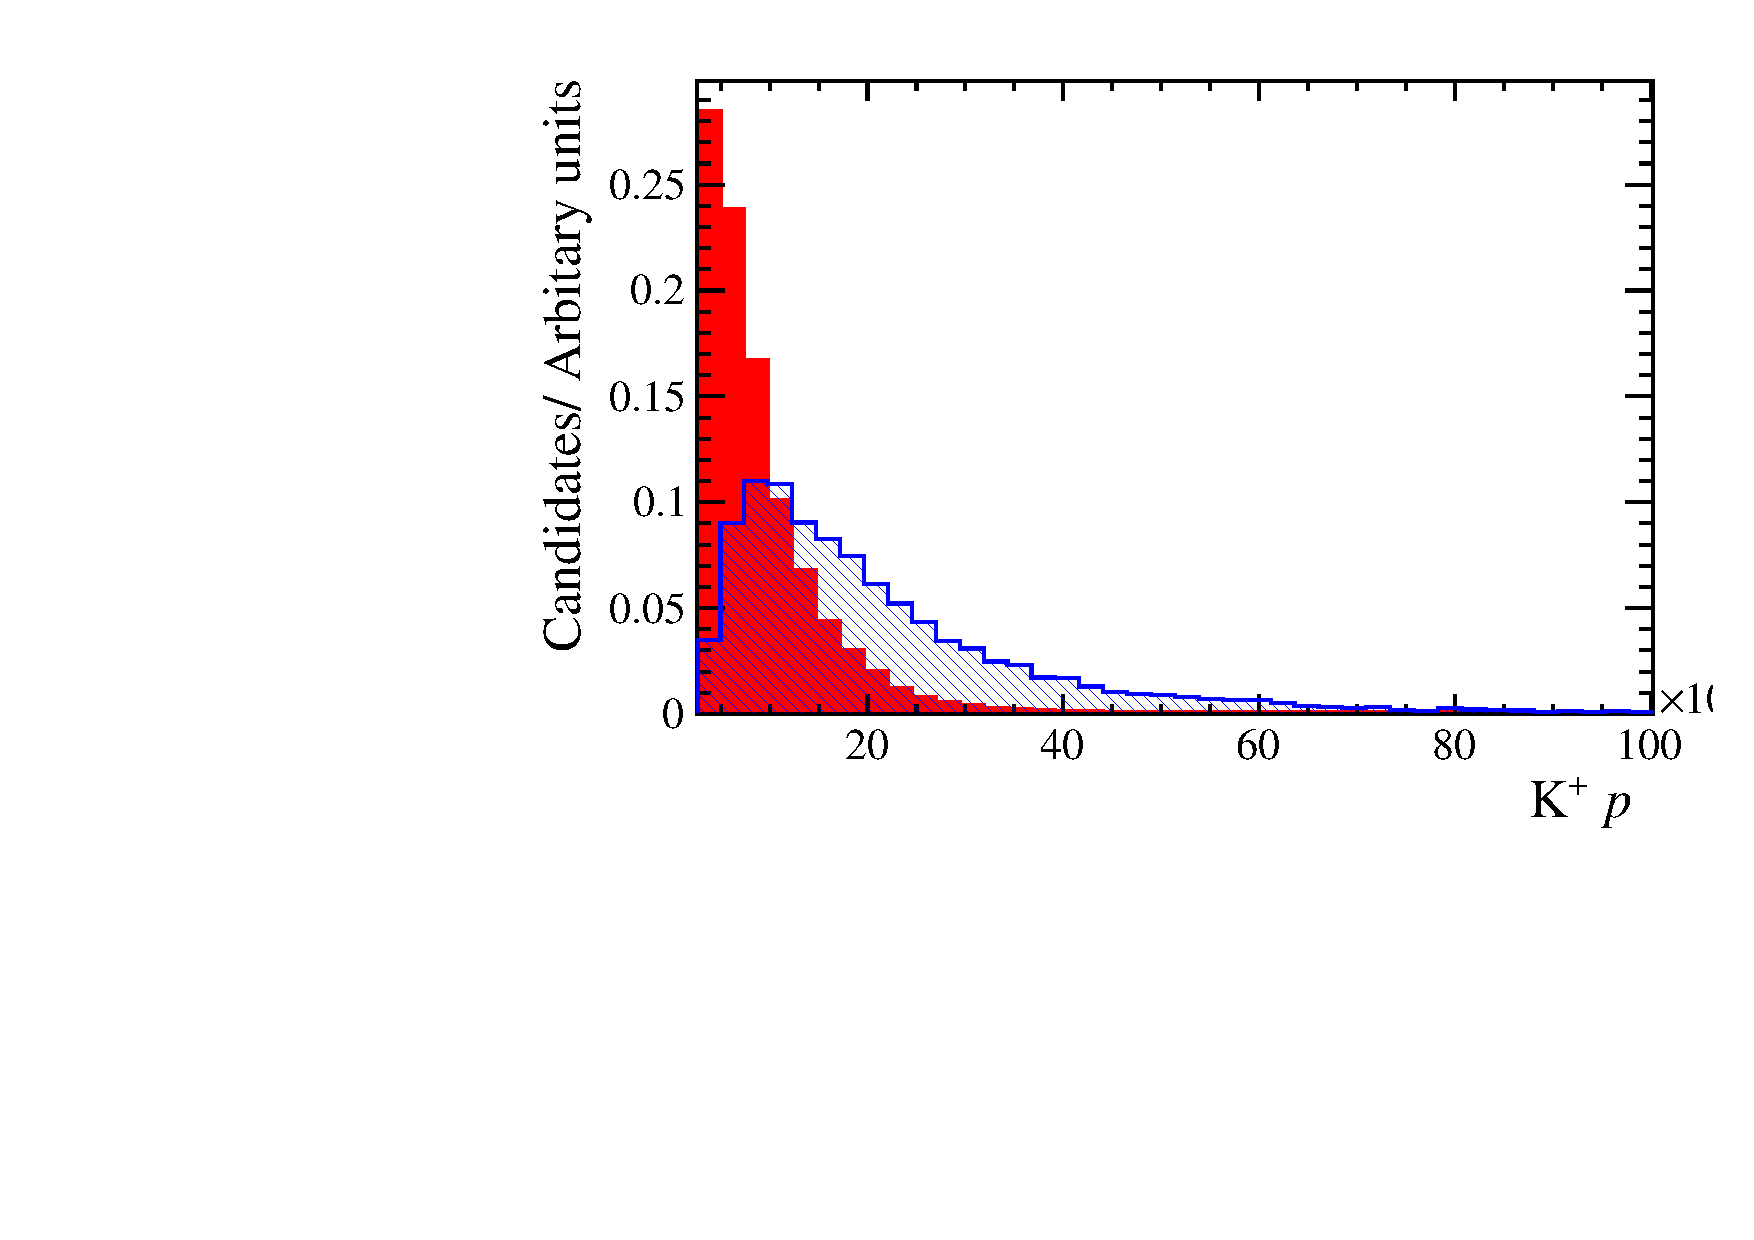
\includegraphics[width=1.0\textwidth]{figs/Selection/Phi_BDT_Var_Ds2KKPi_Phi_K0_P.pdf}
   \end{subfigure}
   \begin{subfigure}[t]{0.22\textwidth}
      \centering
      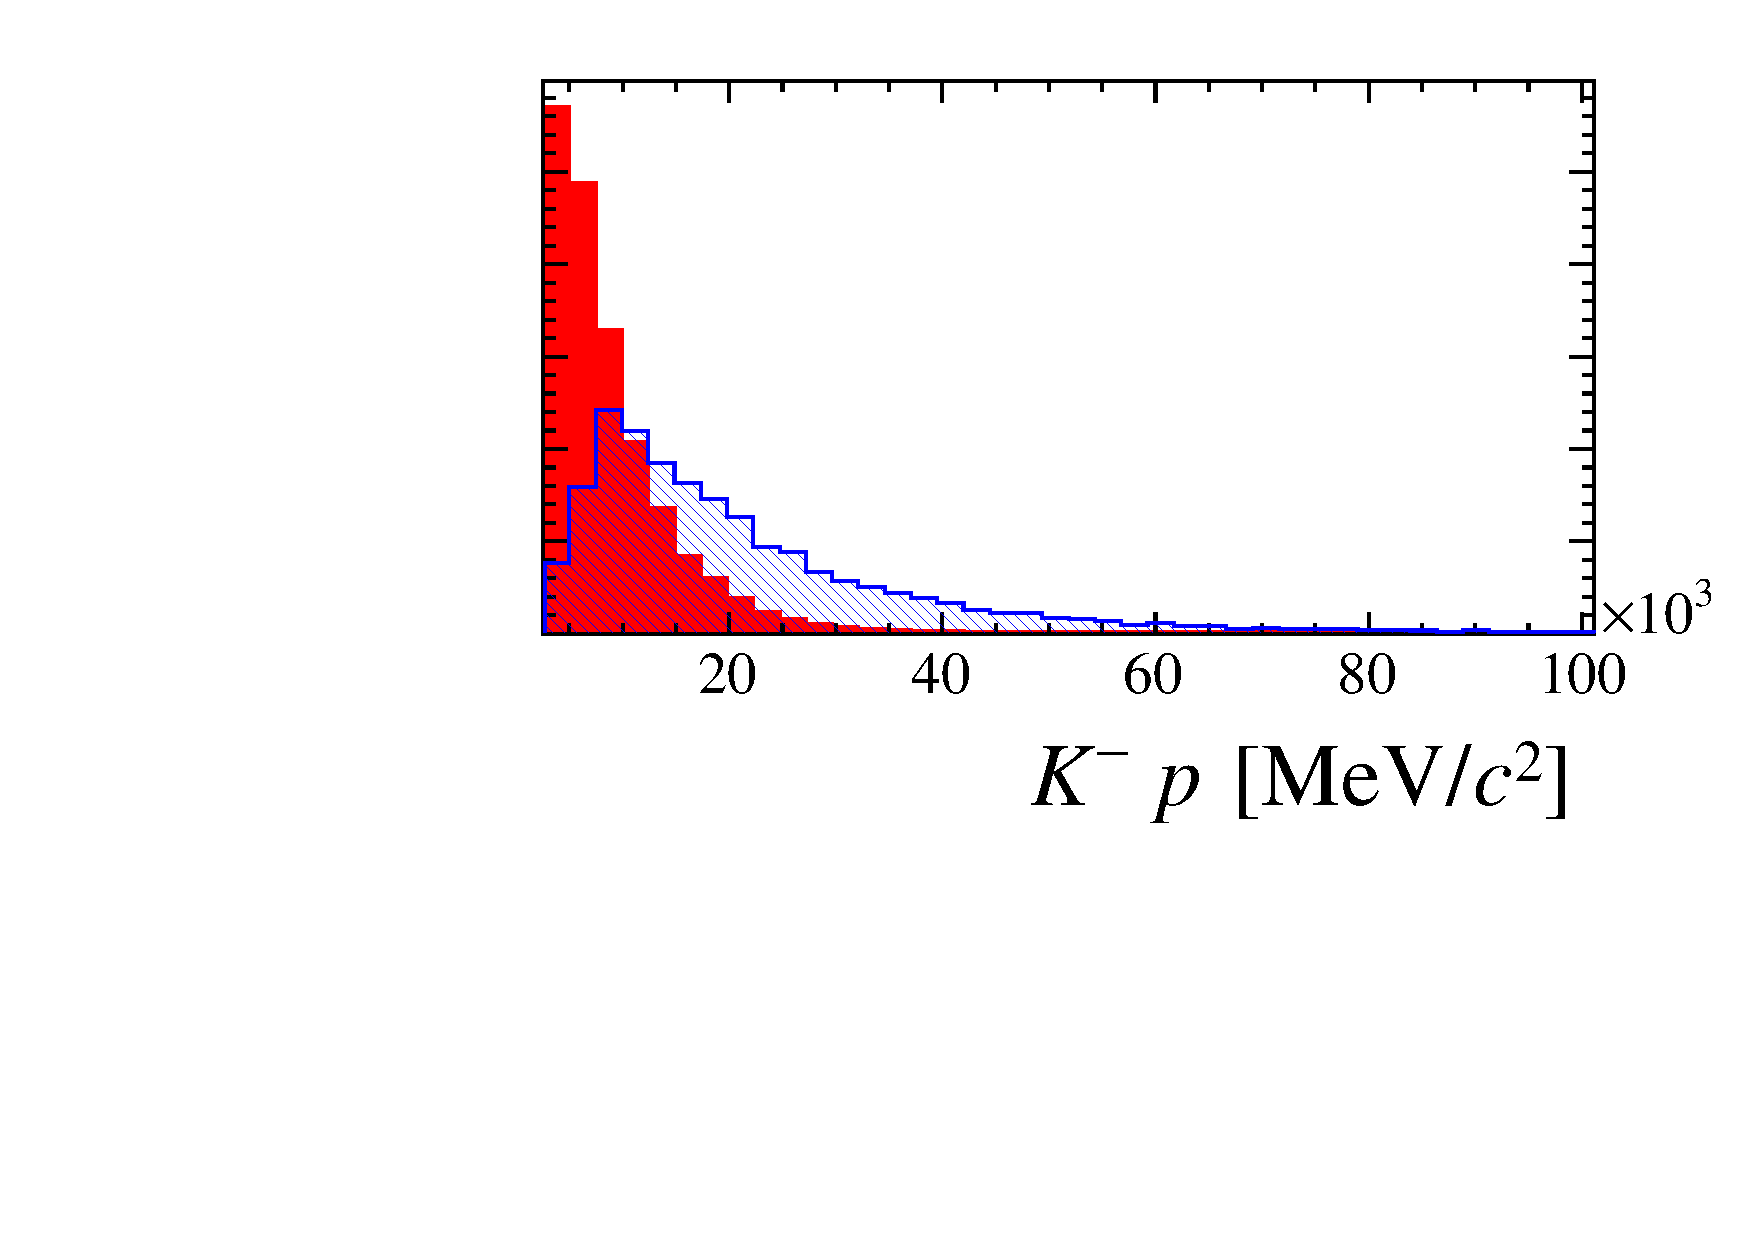
\includegraphics[width=1.0\textwidth]{figs/Selection/Phi_BDT_Var_Ds2KKPi_Phi_K1_P.pdf}
   \end{subfigure}
   \begin{subfigure}[t]{0.22\textwidth}
      \centering
      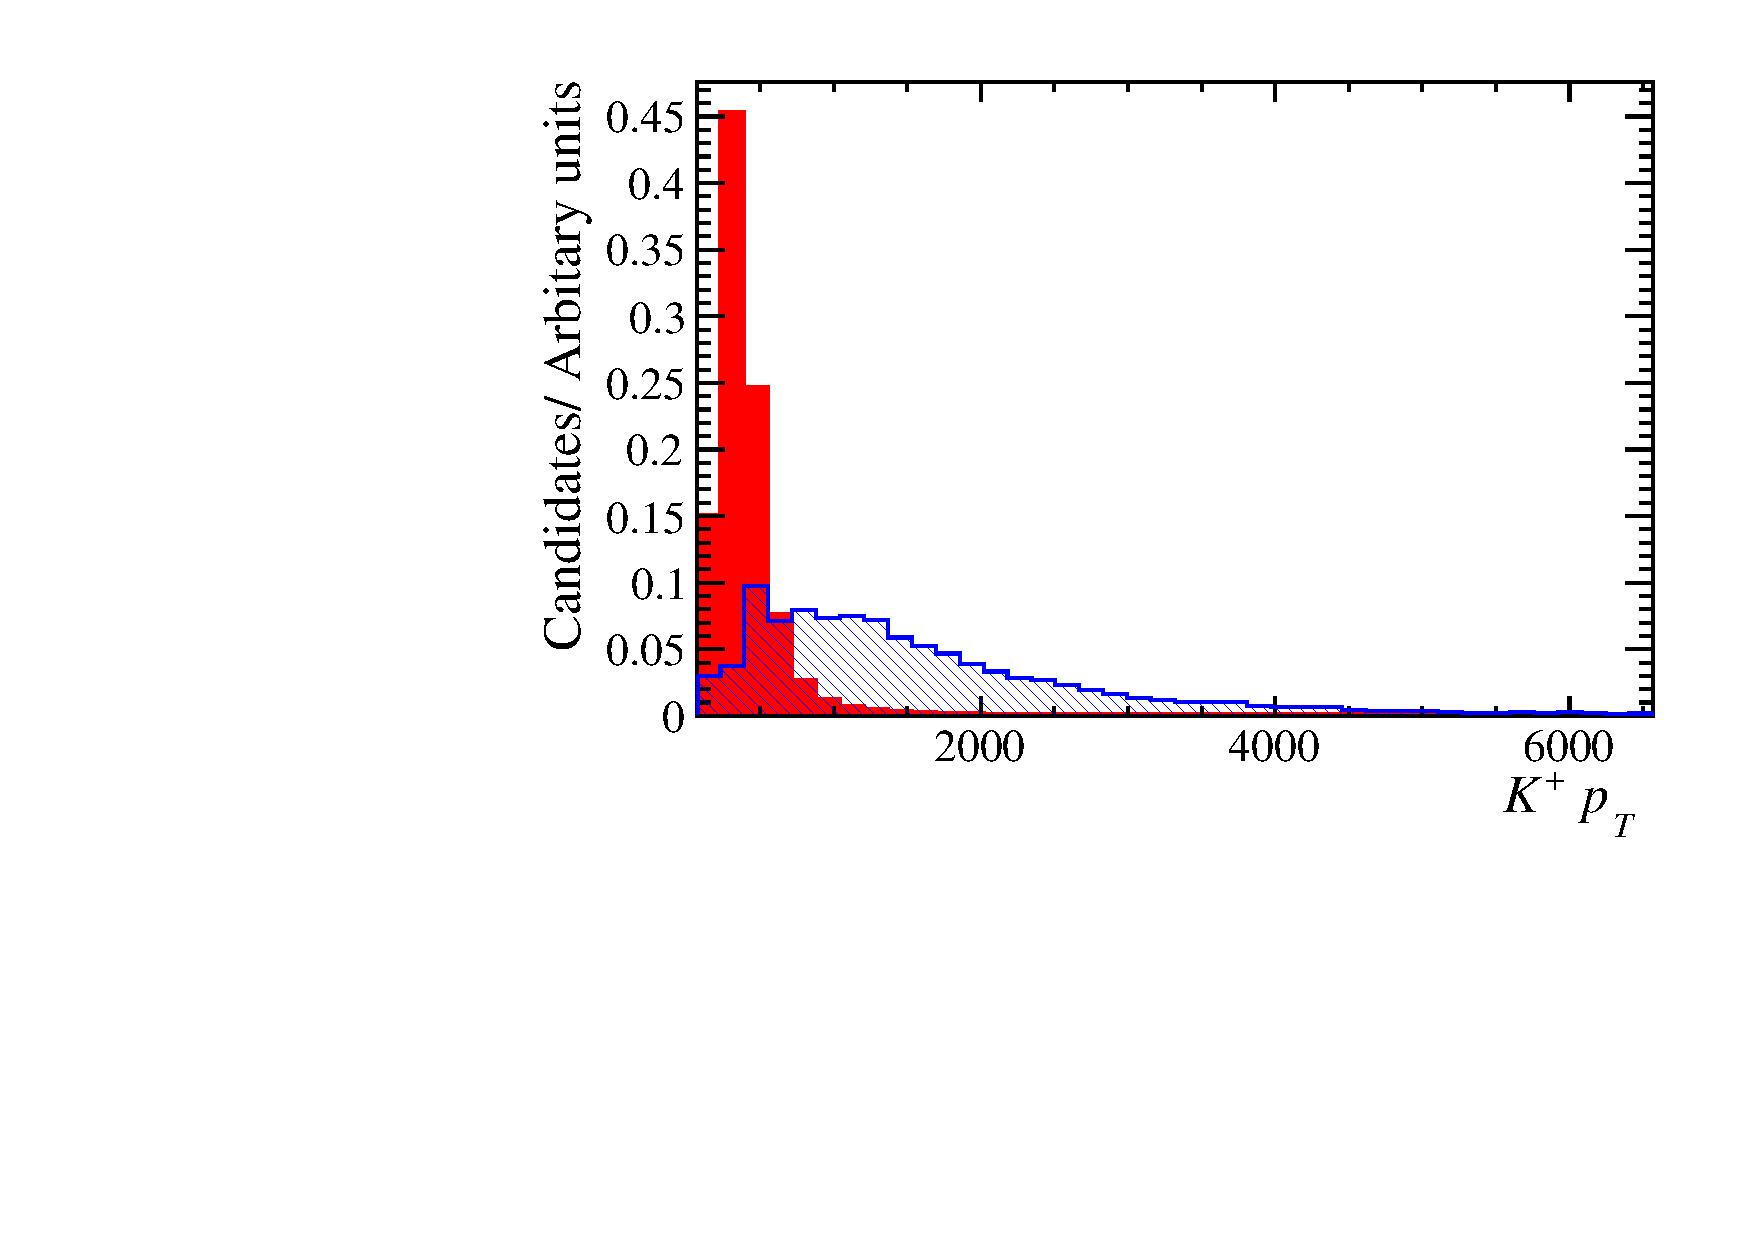
\includegraphics[width=1.0\textwidth]{figs/Selection/Phi_BDT_Var_Ds2KKPi_Phi_K0_PT.pdf}
   \end{subfigure}
   \begin{subfigure}[t]{0.22\textwidth}
      \centering
      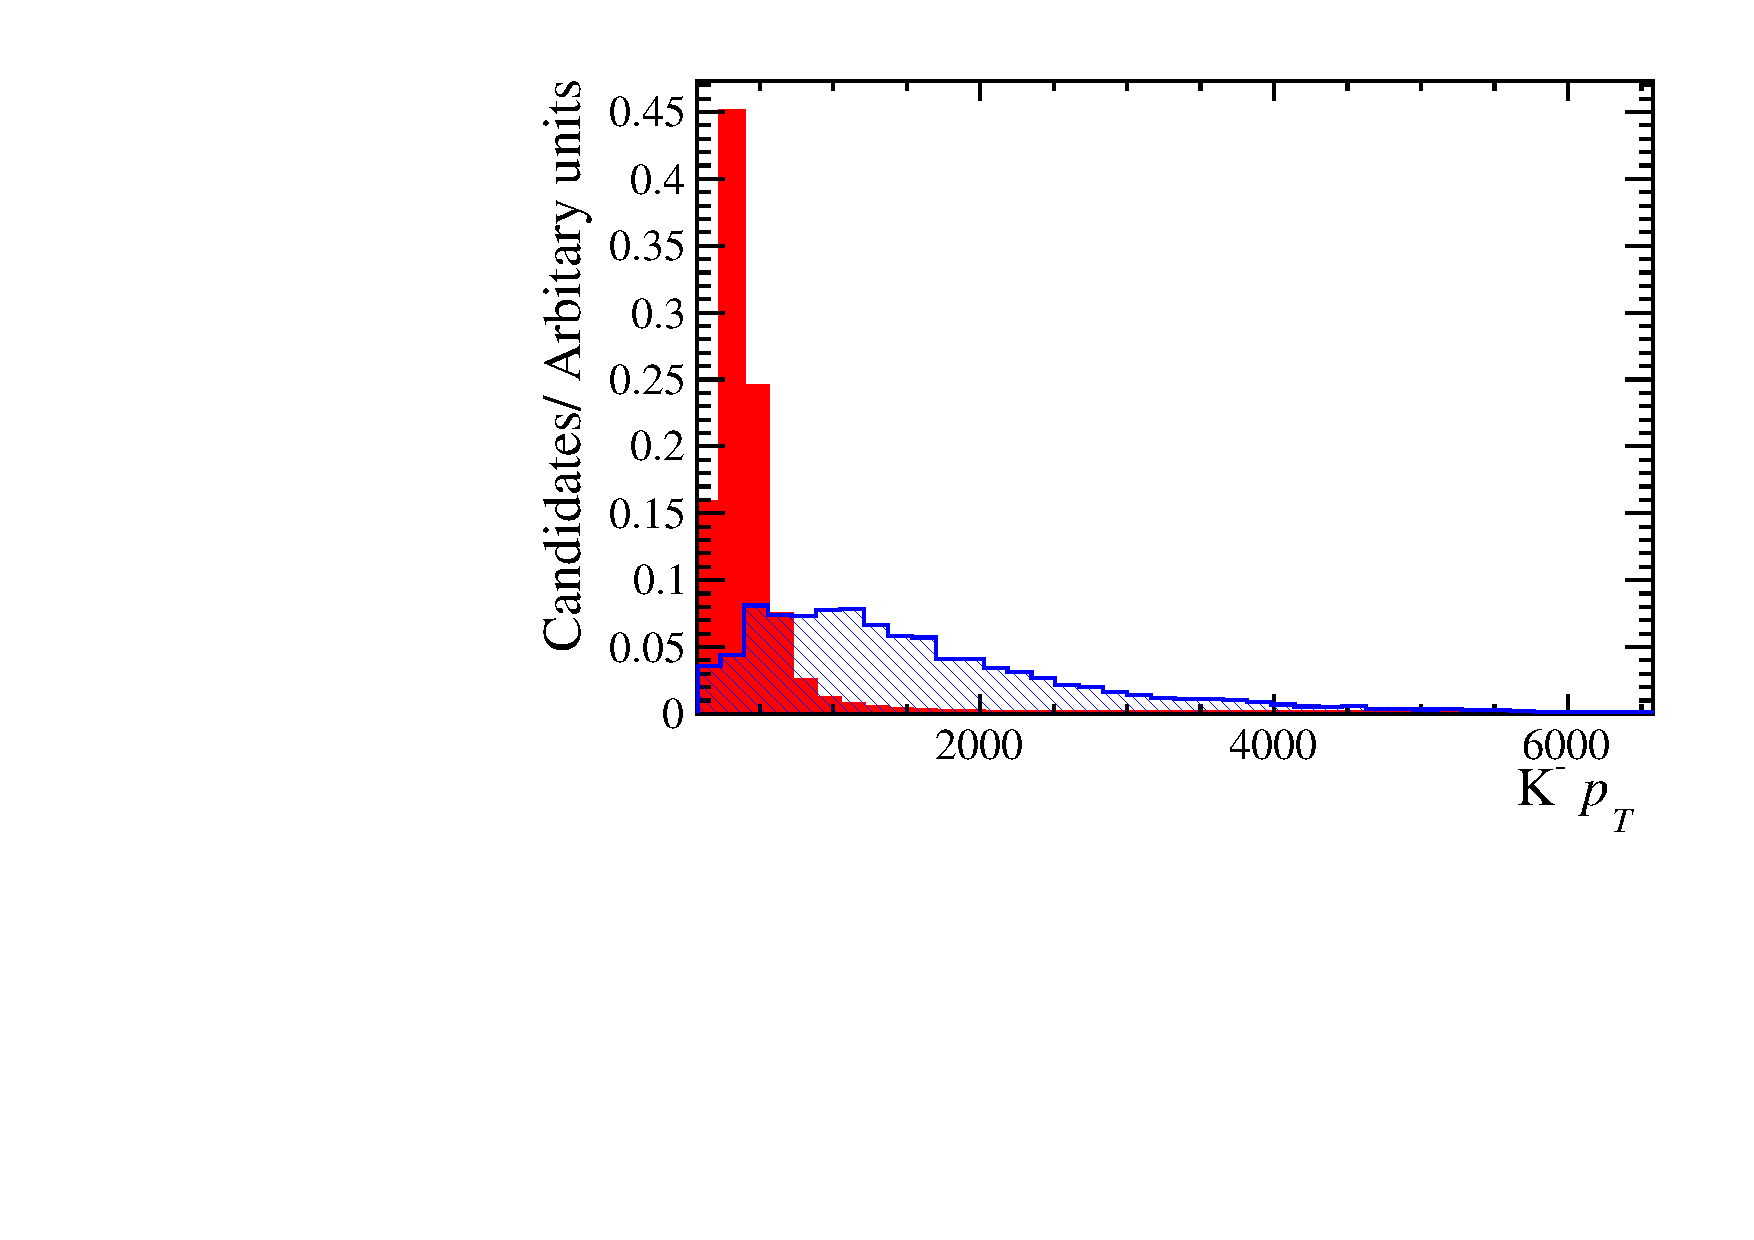
\includegraphics[width=1.0\textwidth]{figs/Selection/Phi_BDT_Var_Ds2KKPi_Phi_K1_PT.pdf}
   \end{subfigure}
   \begin{subfigure}[t]{0.22\textwidth}
      \centering
      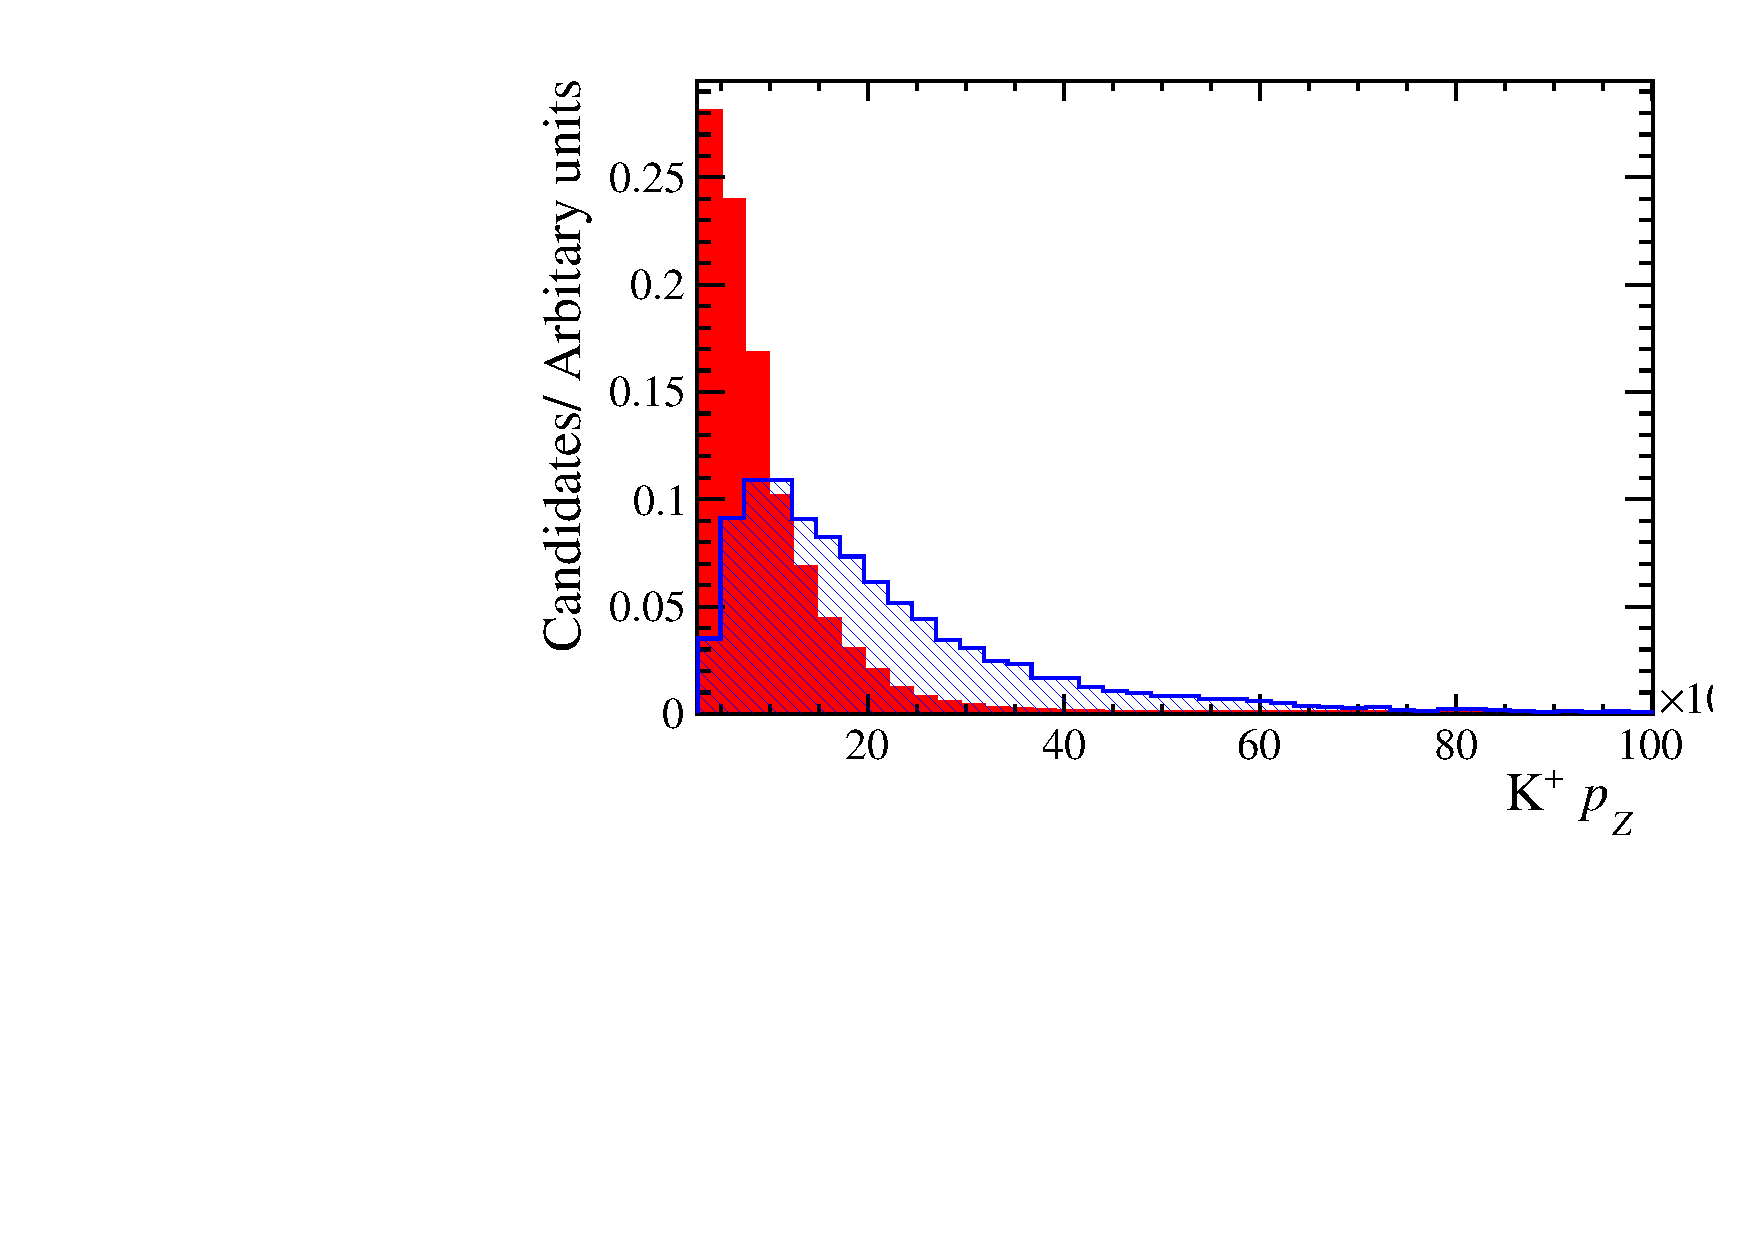
\includegraphics[width=1.0\textwidth]{figs/Selection/Phi_BDT_Var_Ds2KKPi_Phi_K0_PZ.pdf}
   \end{subfigure}
   \begin{subfigure}[t]{0.22\textwidth}
      \centering
      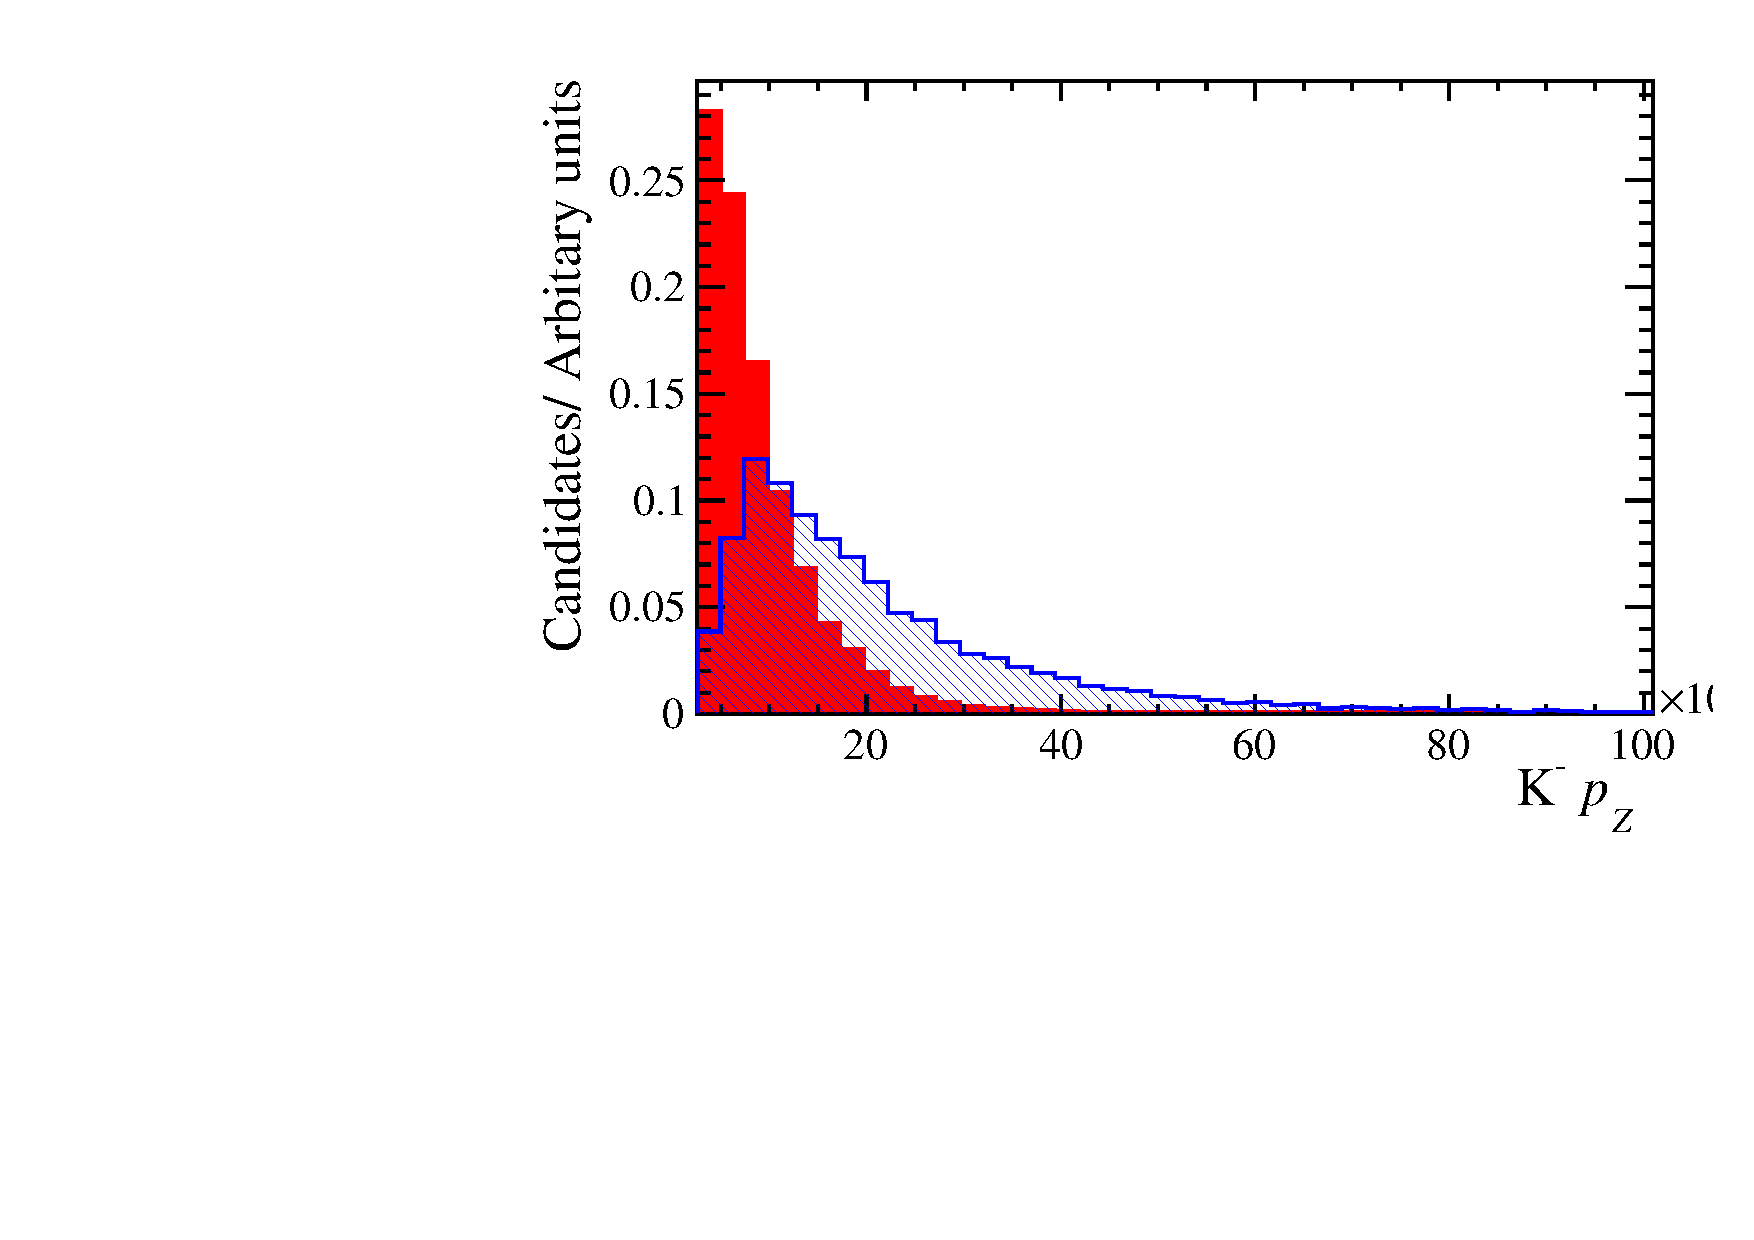
\includegraphics[width=1.0\textwidth]{figs/Selection/Phi_BDT_Var_Ds2KKPi_Phi_K1_PZ.pdf}
   \end{subfigure}
   \begin{subfigure}[t]{0.22\textwidth}
      \centering
      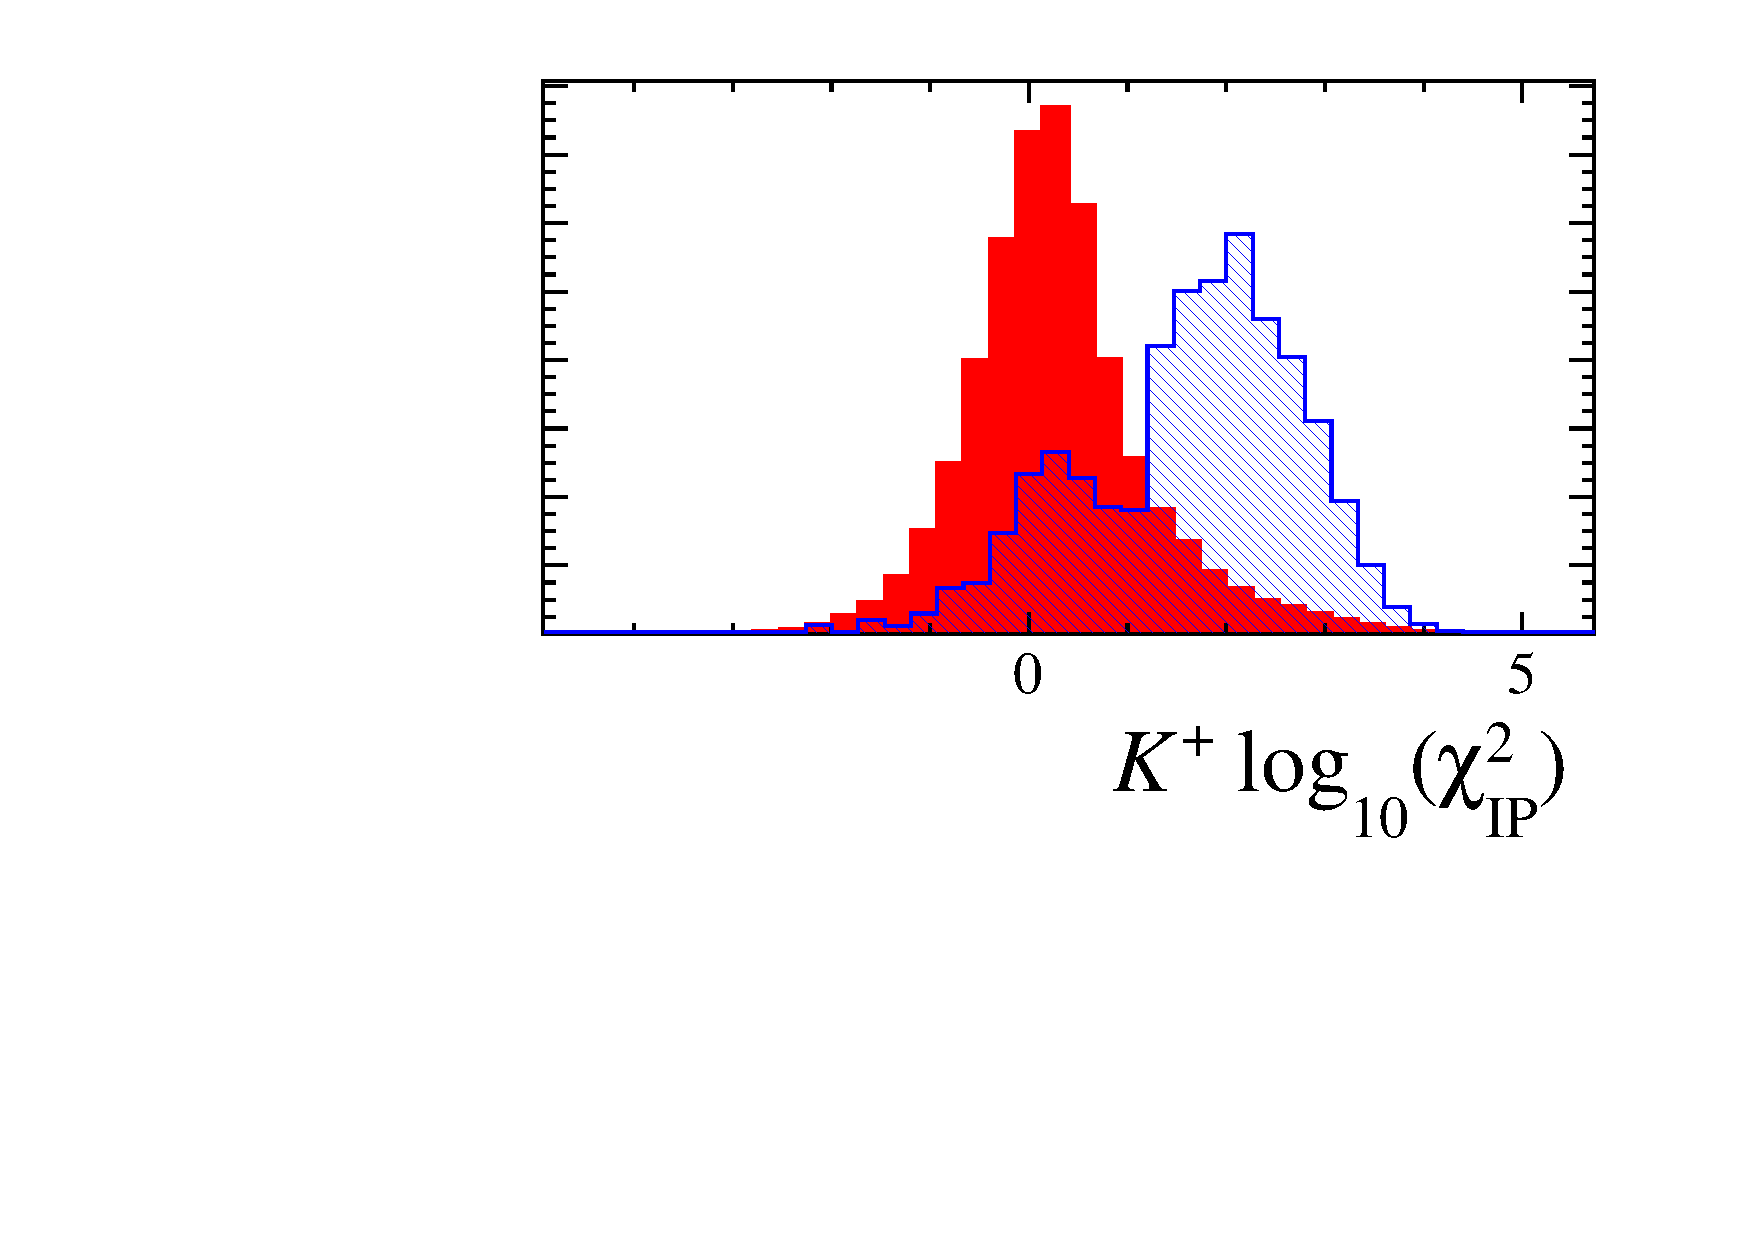
\includegraphics[width=1.0\textwidth]{figs/Selection/Phi_BDT_Var_Ds2KKPi_log10_Phi_K0_IPCHI2_OWNPV.pdf}
   \end{subfigure}
   \begin{subfigure}[t]{0.22\textwidth}
      \centering
      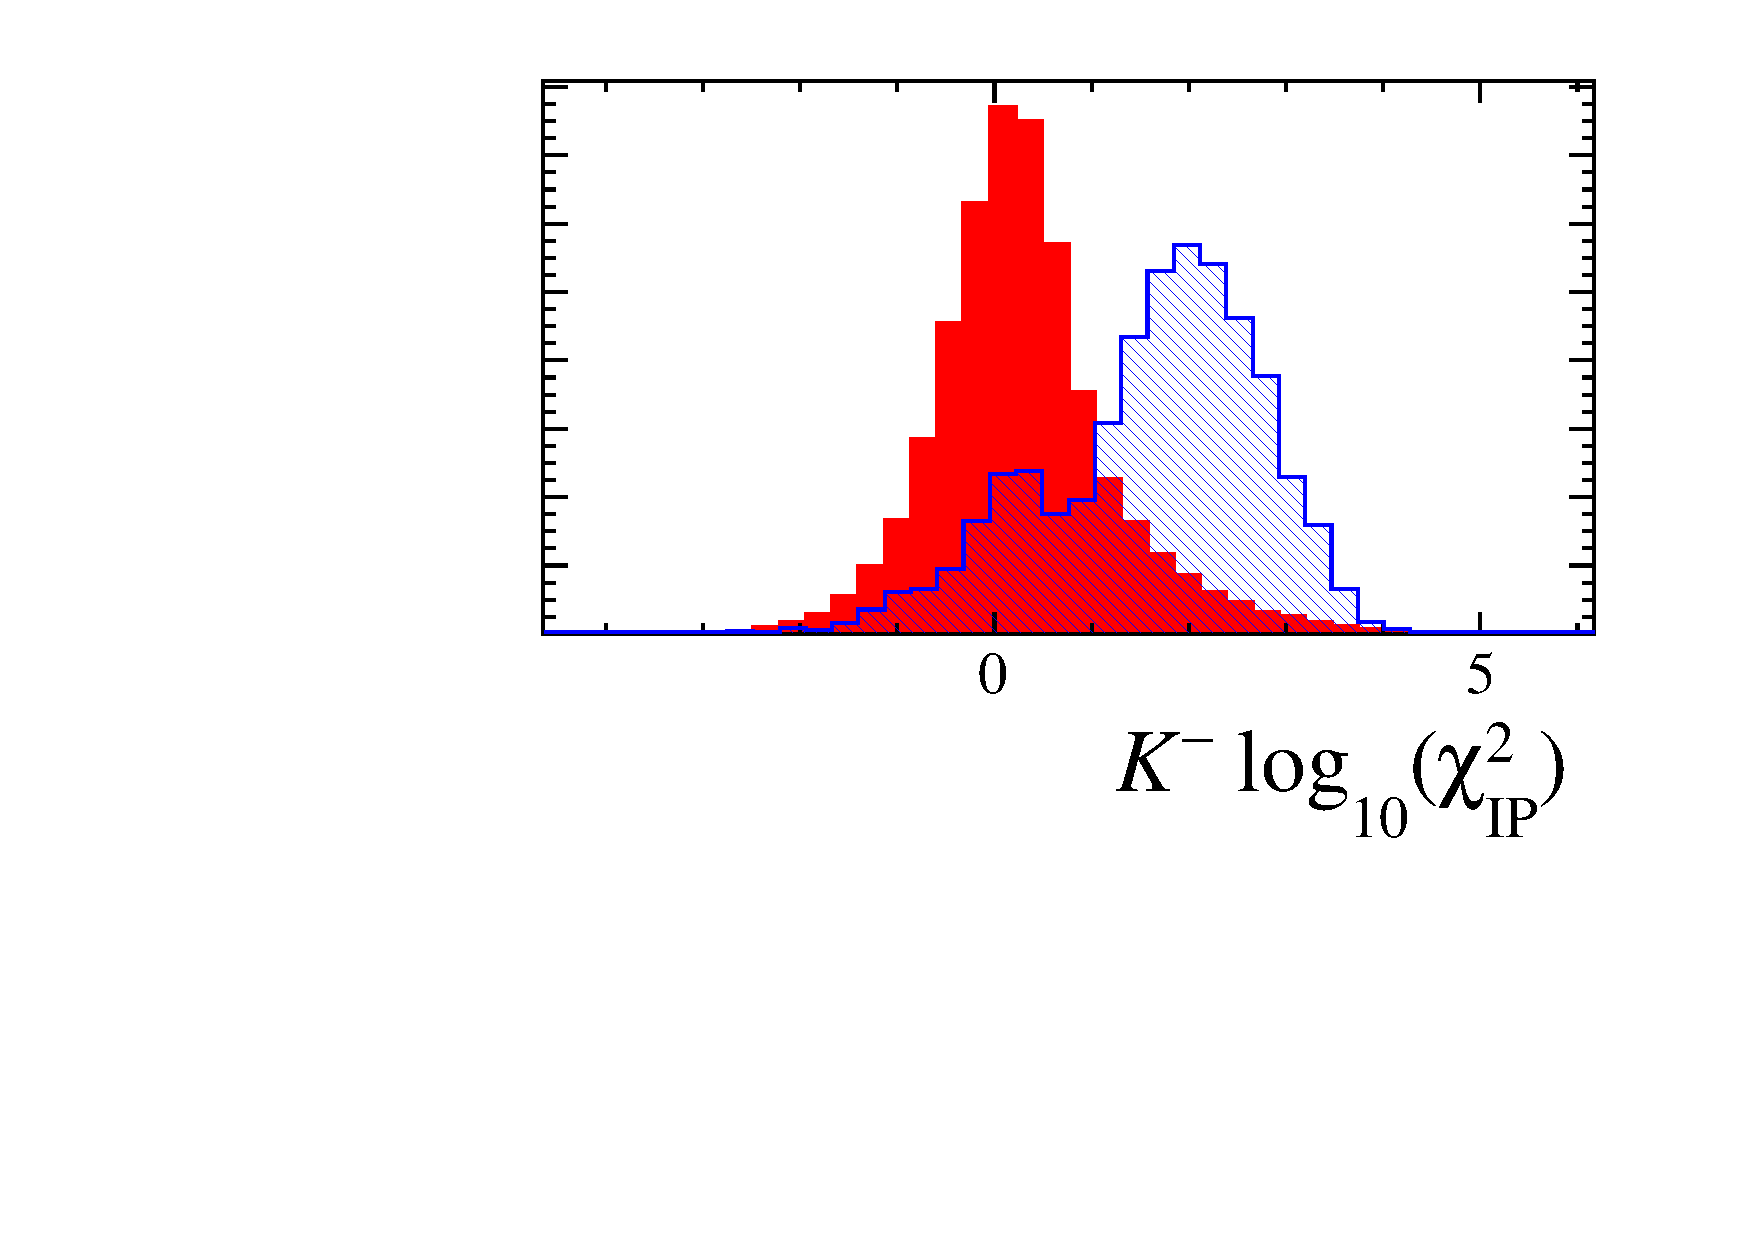
\includegraphics[width=1.0\textwidth]{figs/Selection/Phi_BDT_Var_Ds2KKPi_log10_Phi_K1_IPCHI2_OWNPV.pdf}
   \end{subfigure}
   \begin{subfigure}[t]{0.22\textwidth}
      \centering
      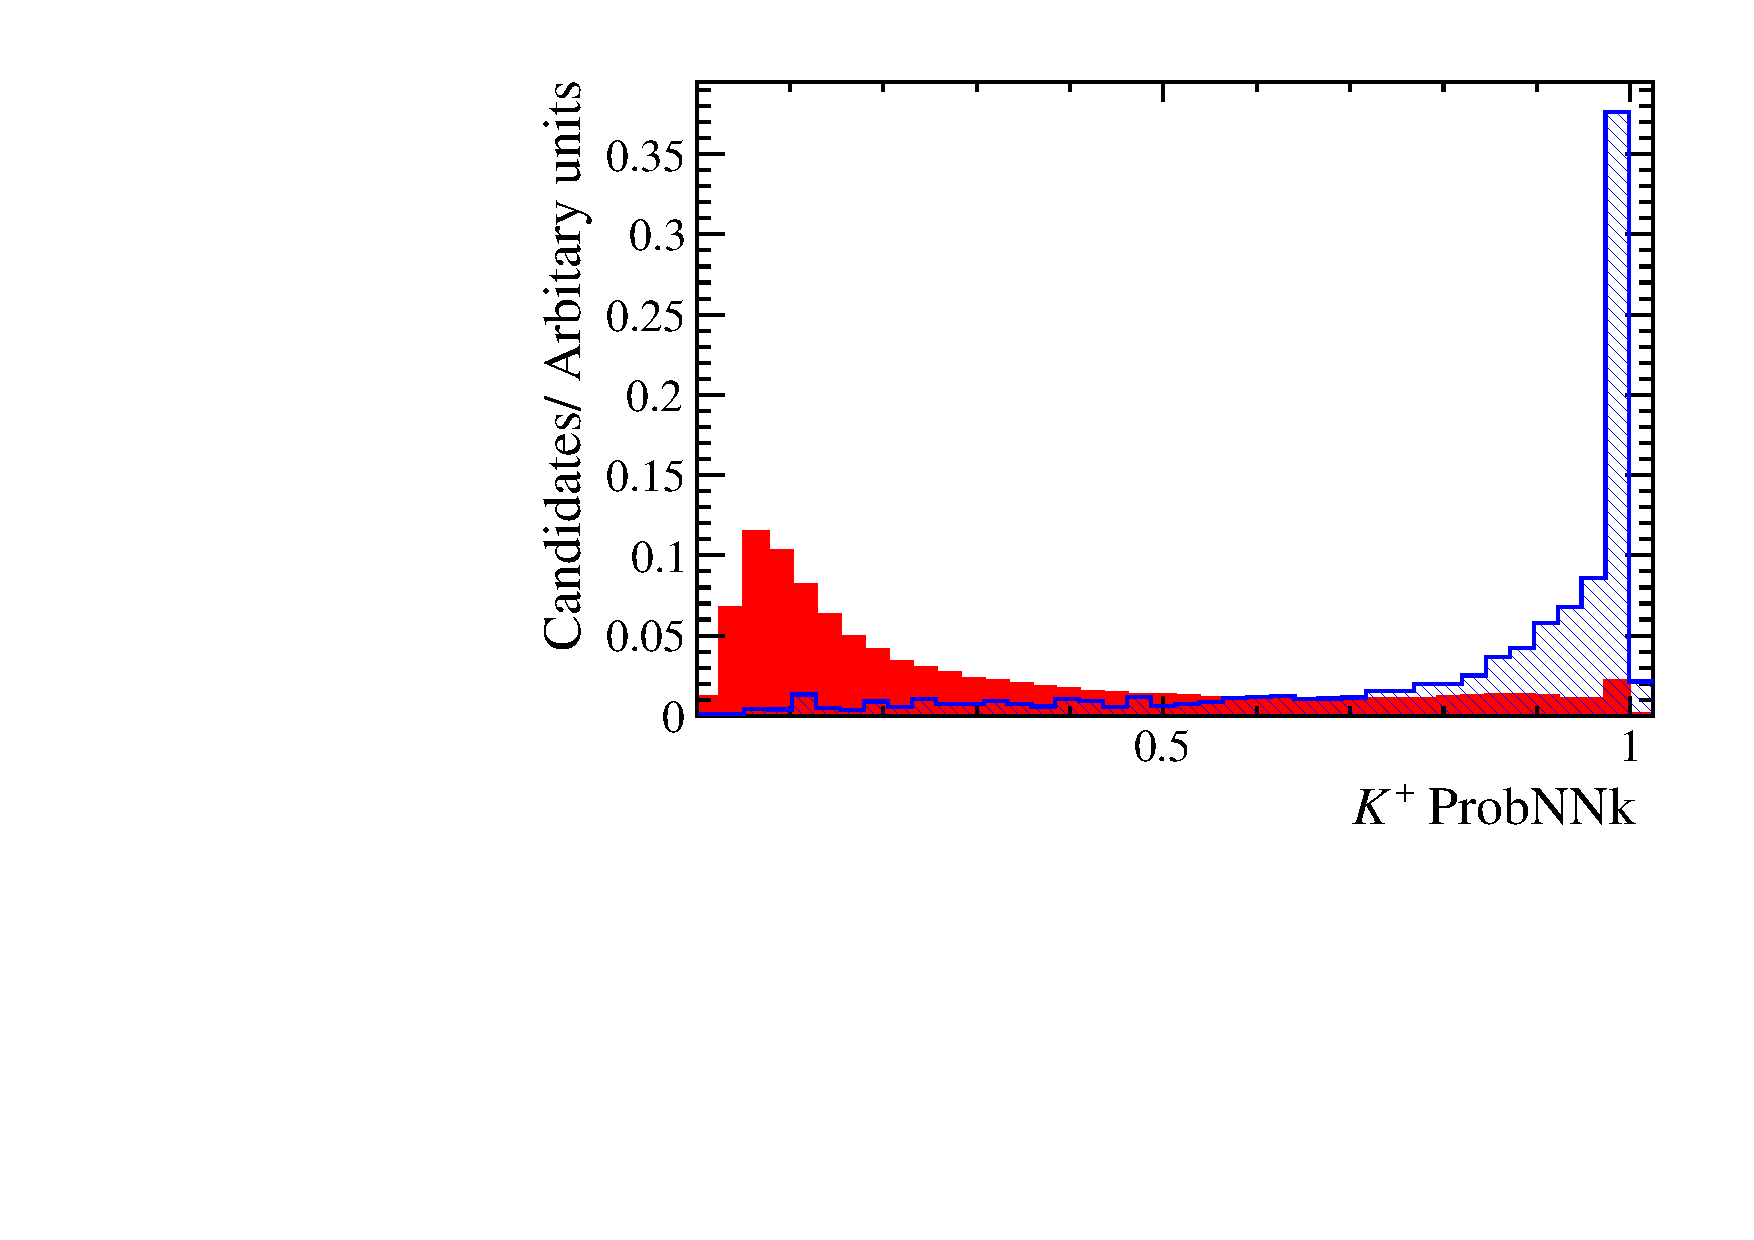
\includegraphics[width=1.0\textwidth]{figs/Selection/Phi_BDT_Var_Ds2KKPi_Phi_K0_MC15TuneV1_ProbNNk.pdf}
   \end{subfigure}
   \begin{subfigure}[t]{0.22\textwidth}
      \centering
      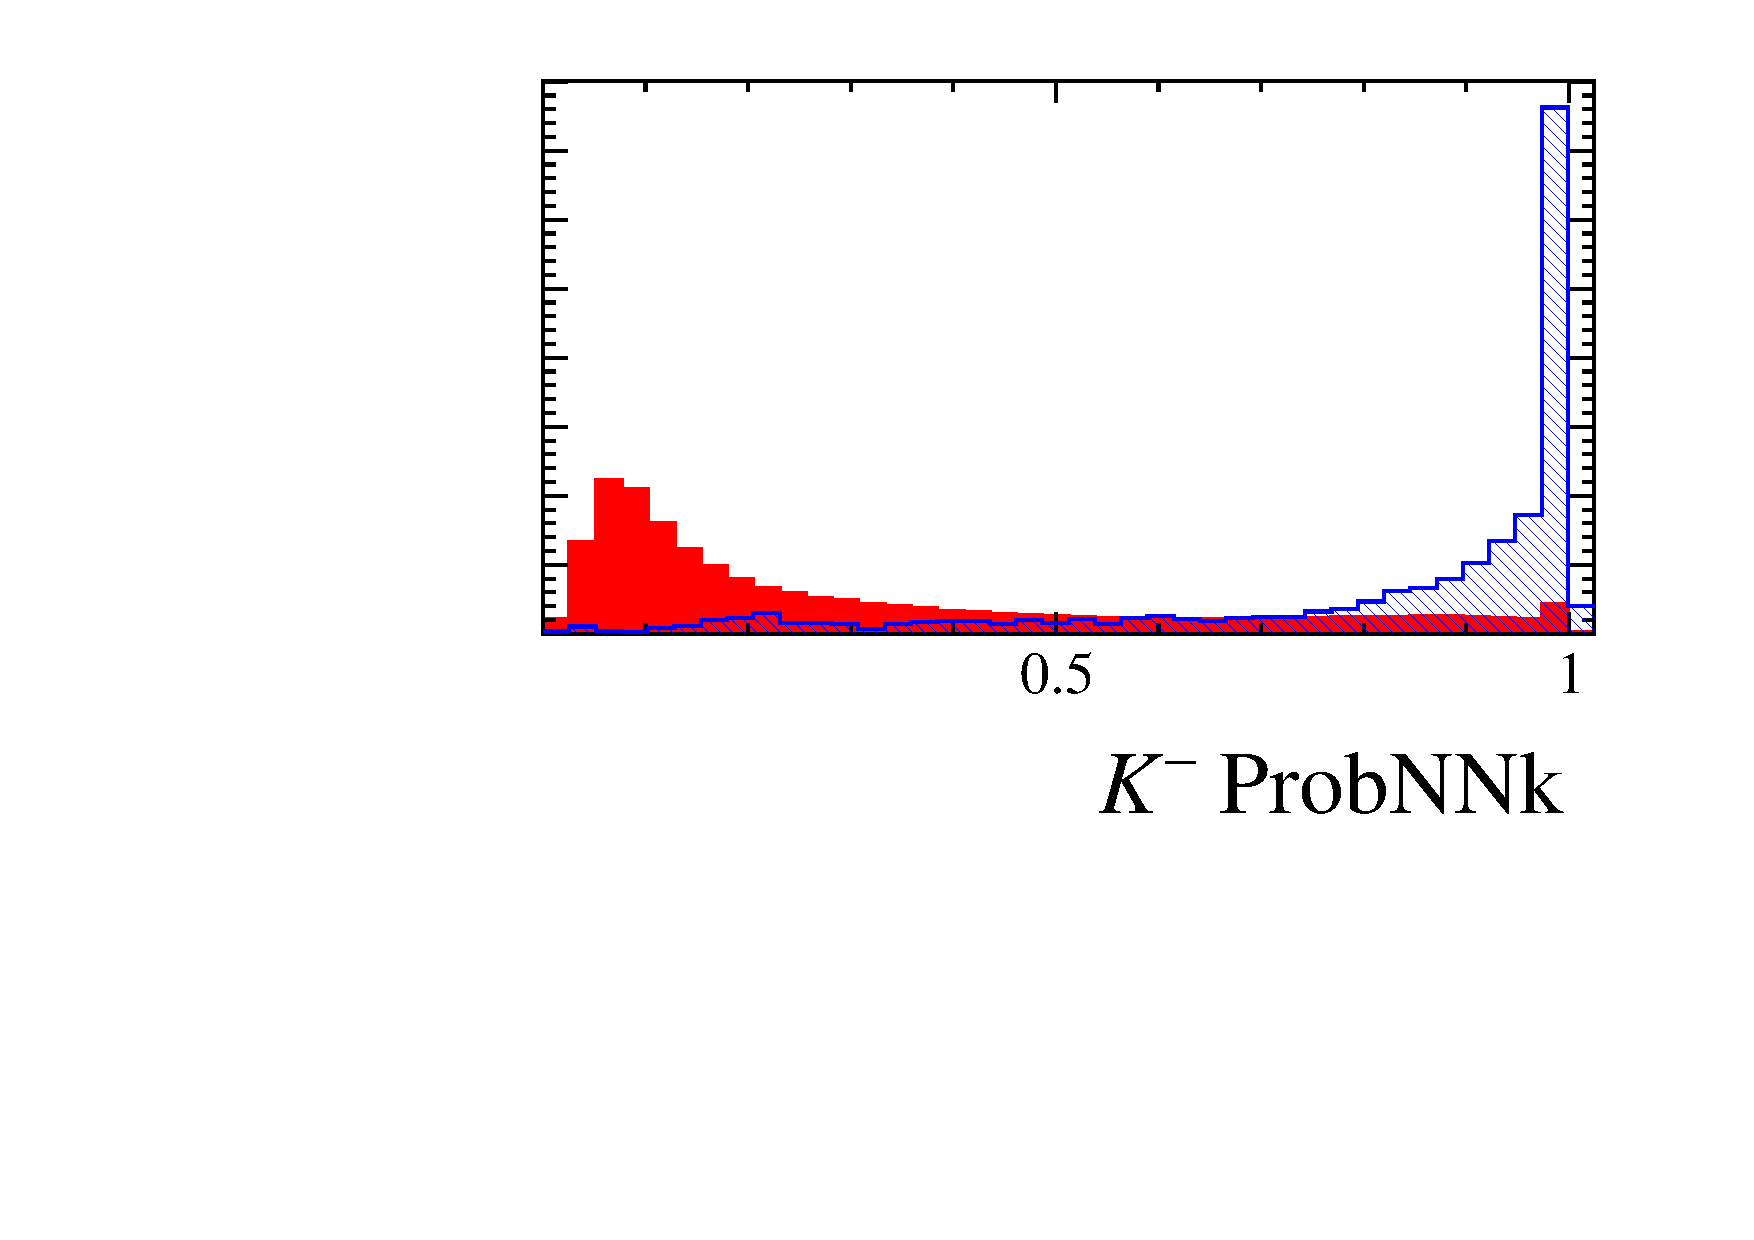
\includegraphics[width=1.0\textwidth]{figs/Selection/Phi_BDT_Var_Ds2KKPi_Phi_K1_MC15TuneV1_ProbNNk.pdf}
   \end{subfigure}
   \begin{subfigure}[t]{0.22\textwidth}
      \centering
      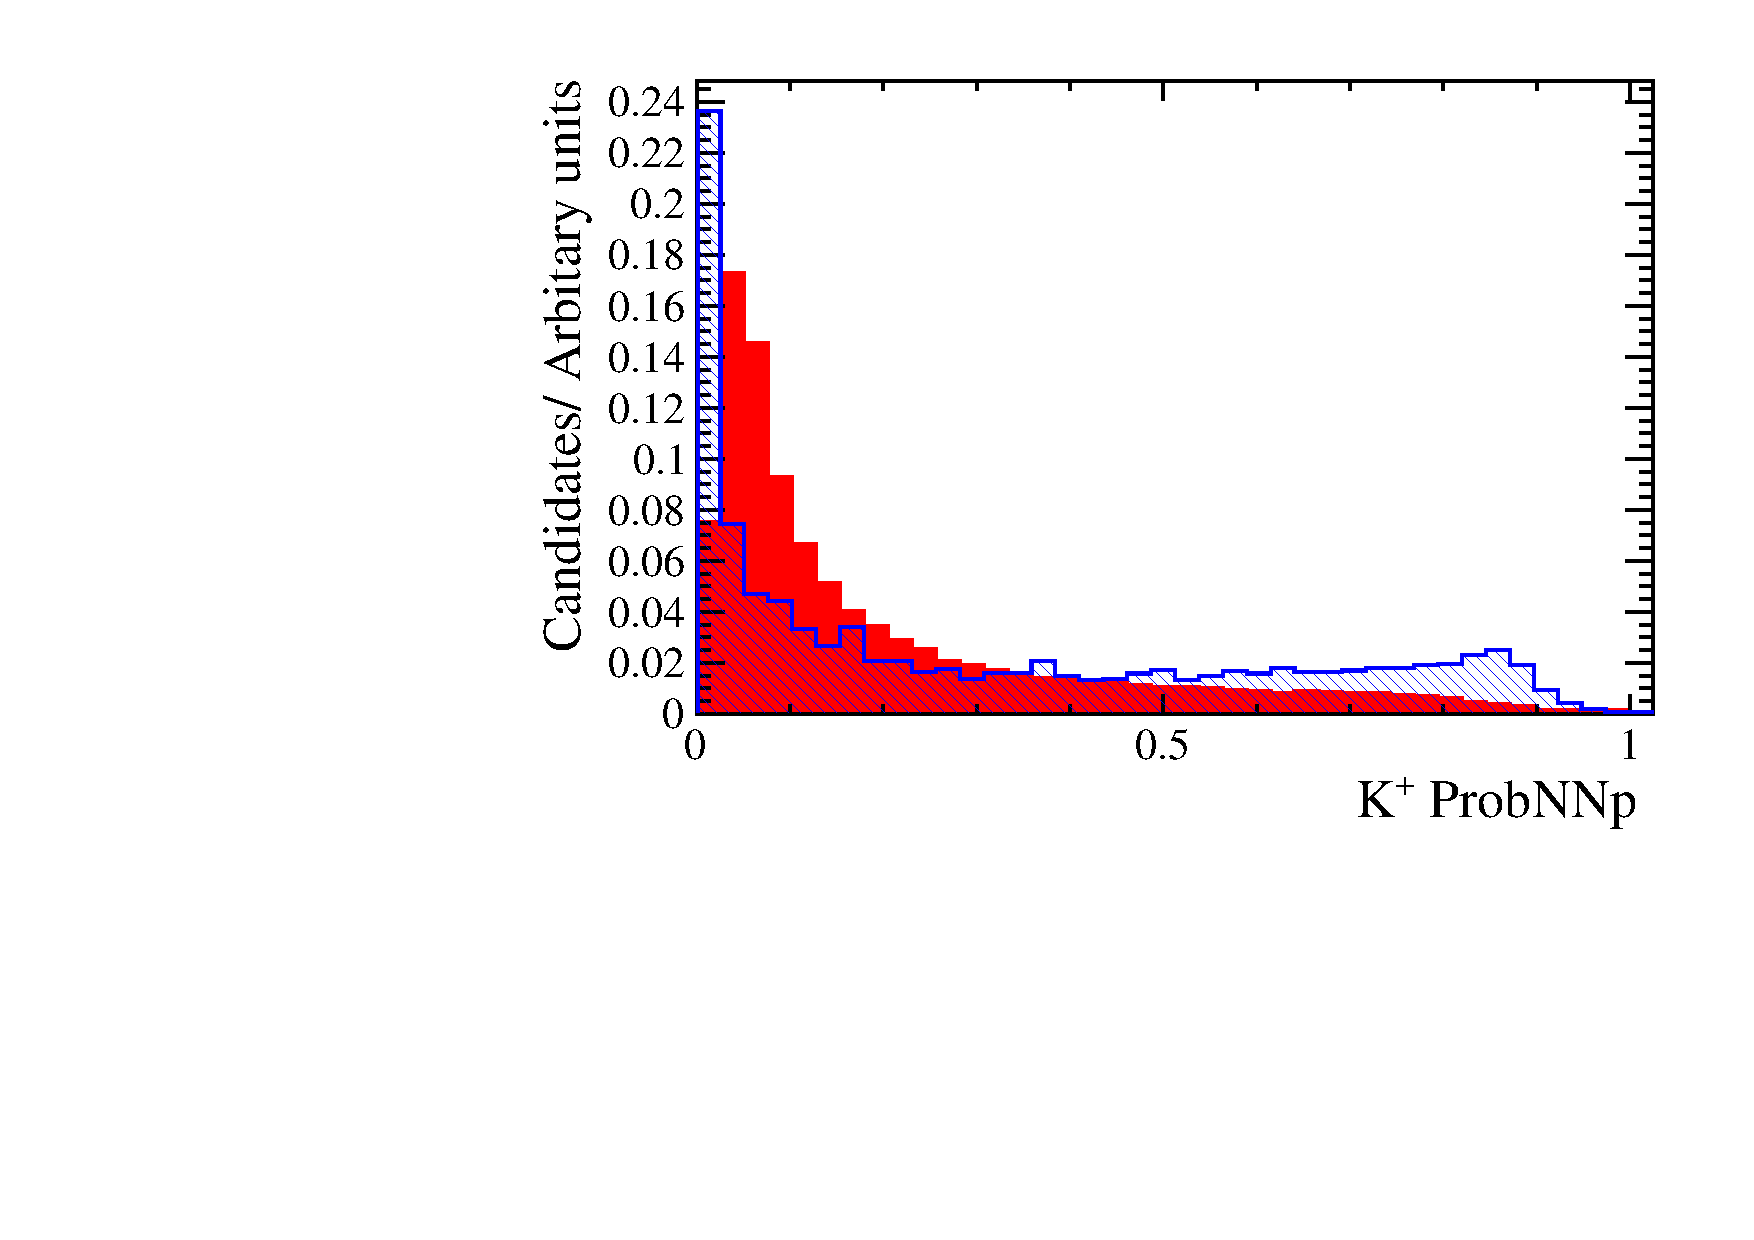
\includegraphics[width=1.0\textwidth]{figs/Selection/Phi_BDT_Var_Ds2KKPi_Phi_K0_MC15TuneV1_ProbNNp.pdf}
   \end{subfigure}
   \begin{subfigure}[t]{0.22\textwidth}
      \centering
      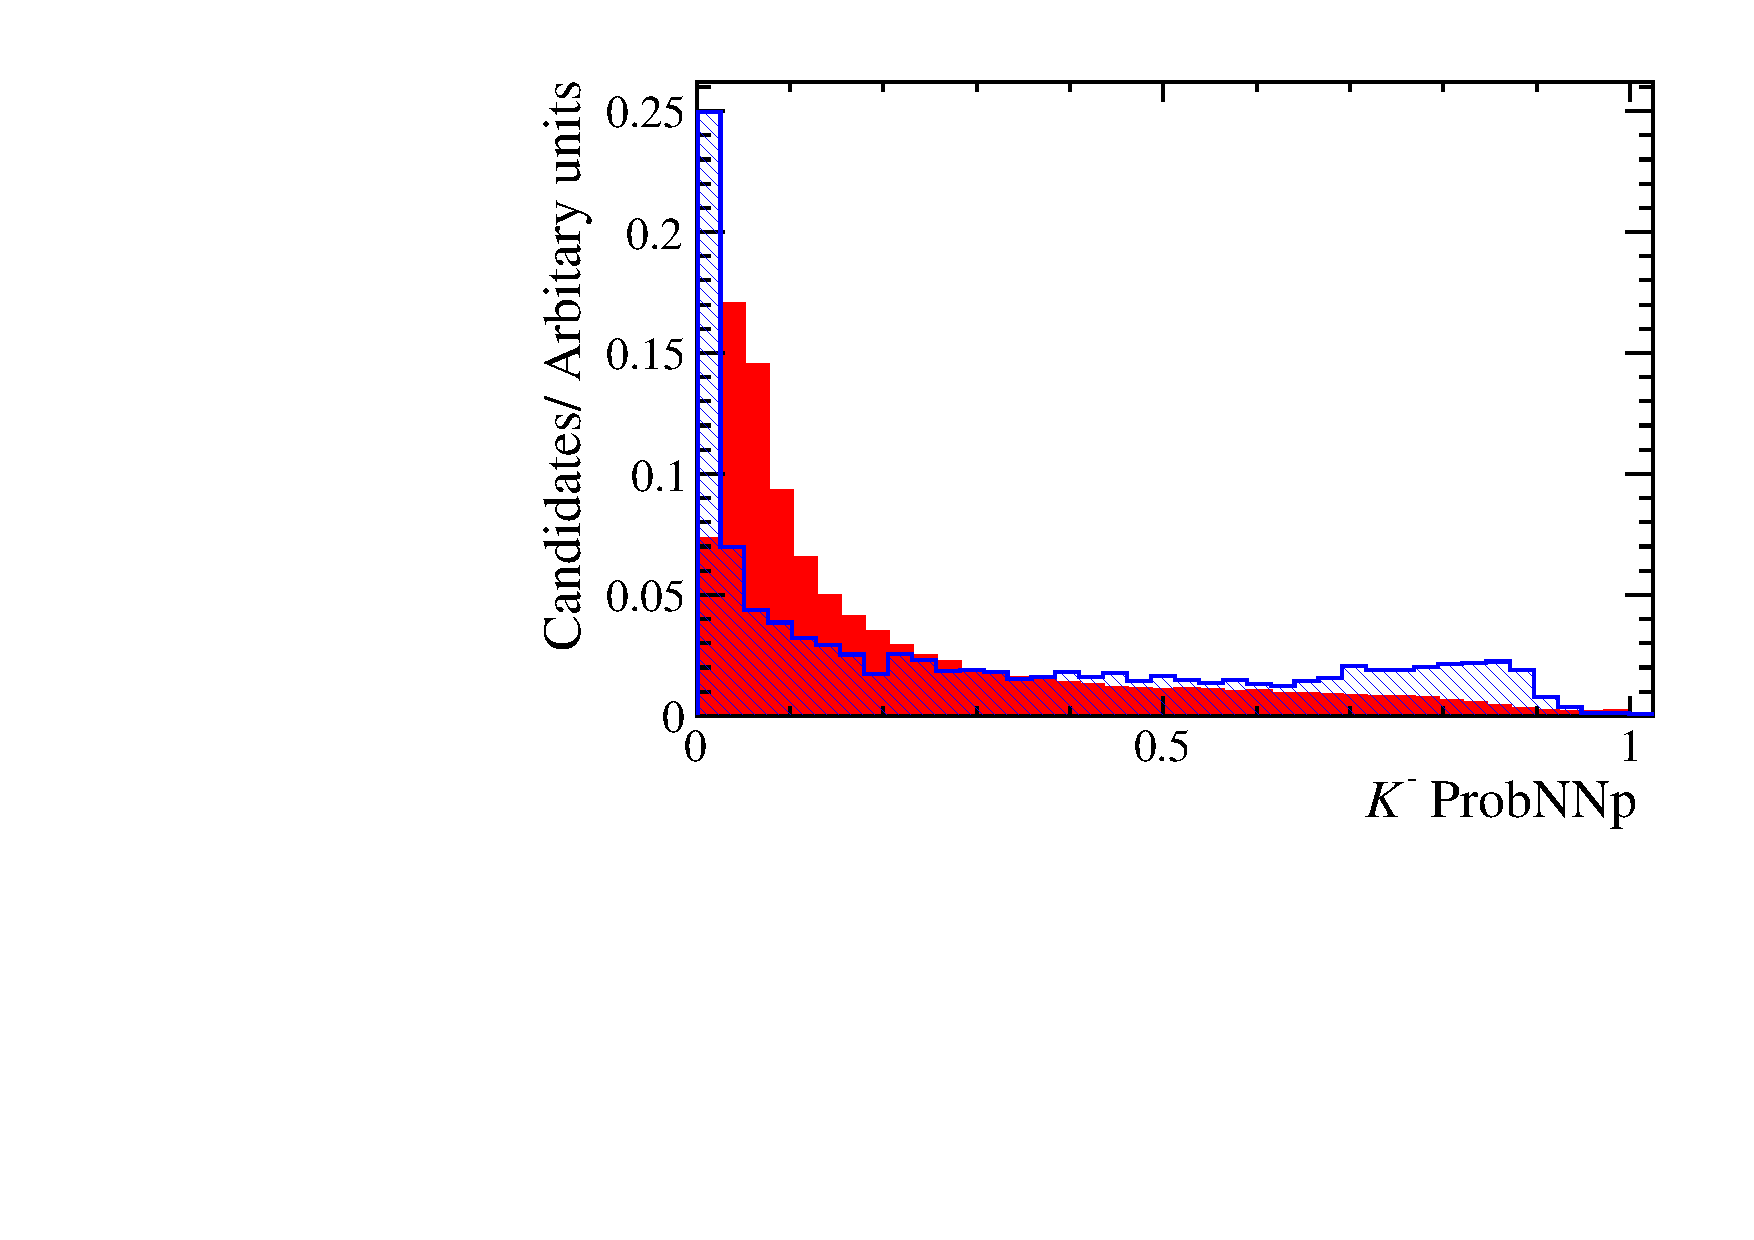
\includegraphics[width=1.0\textwidth]{figs/Selection/Phi_BDT_Var_Ds2KKPi_Phi_K1_MC15TuneV1_ProbNNp.pdf}
   \end{subfigure}
   \begin{subfigure}[t]{0.22\textwidth}
      \centering
      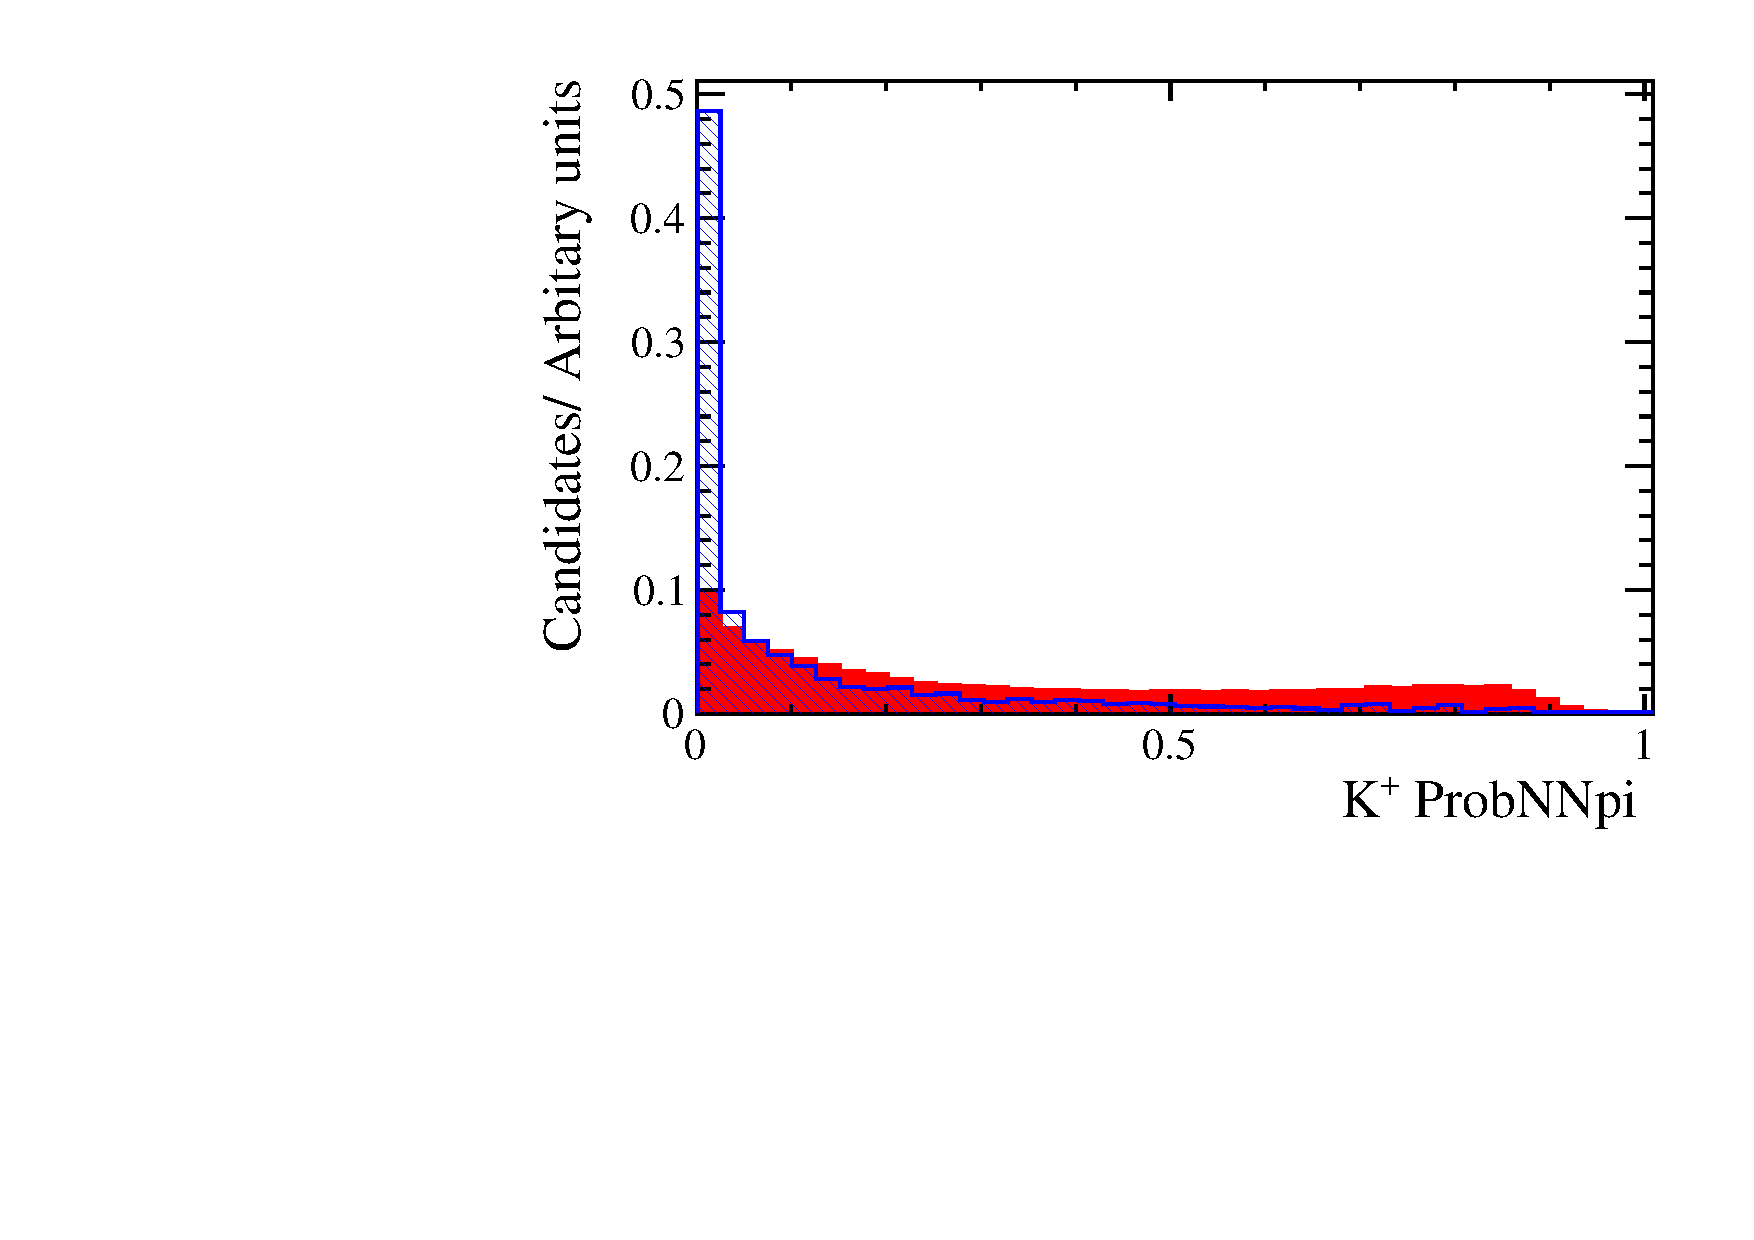
\includegraphics[width=1.0\textwidth]{figs/Selection/Phi_BDT_Var_Ds2KKPi_Phi_K0_MC15TuneV1_ProbNNpi.pdf}
   \end{subfigure}
   \begin{subfigure}[t]{0.22\textwidth}
      \centering
      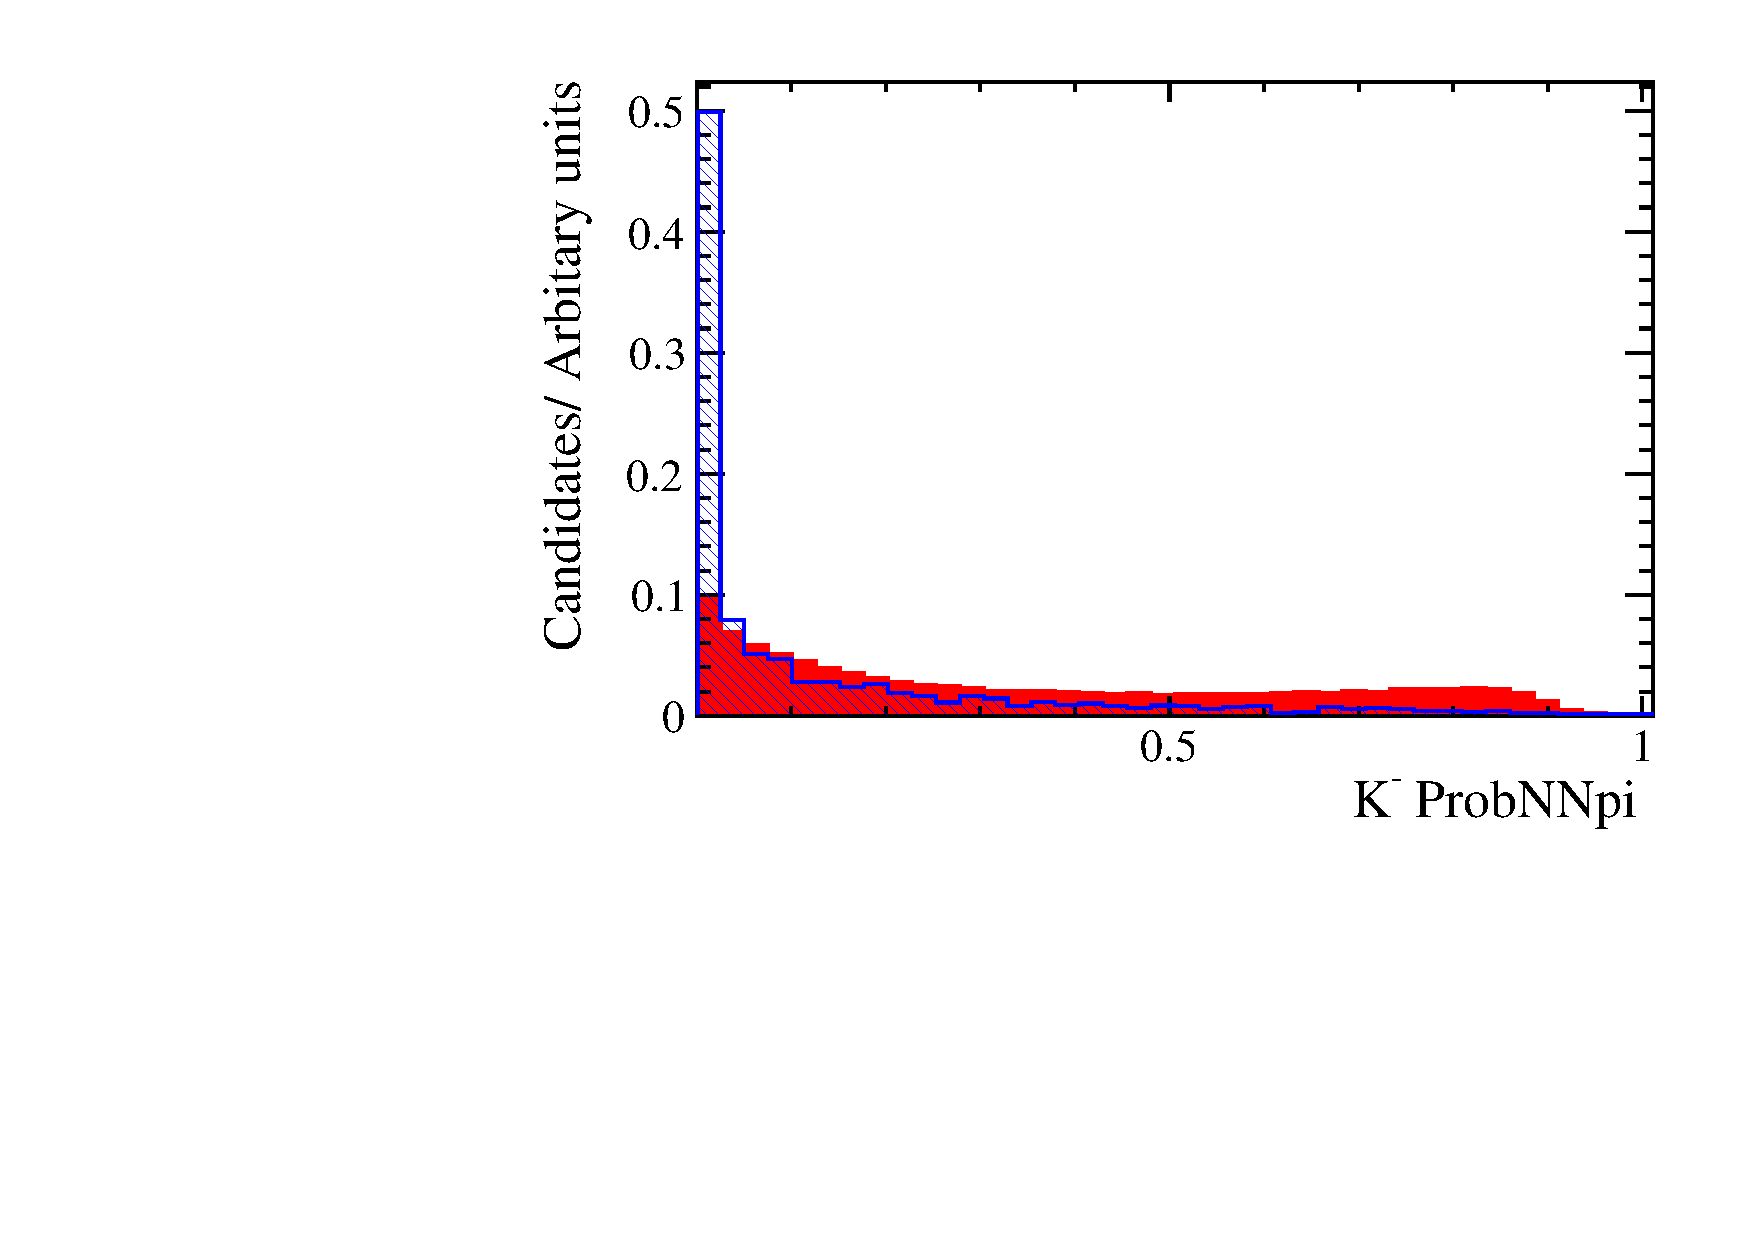
\includegraphics[width=1.0\textwidth]{figs/Selection/Phi_BDT_Var_Ds2KKPi_Phi_K1_MC15TuneV1_ProbNNpi.pdf}
   \end{subfigure}
   \begin{subfigure}[t]{0.22\textwidth}
      \centering
      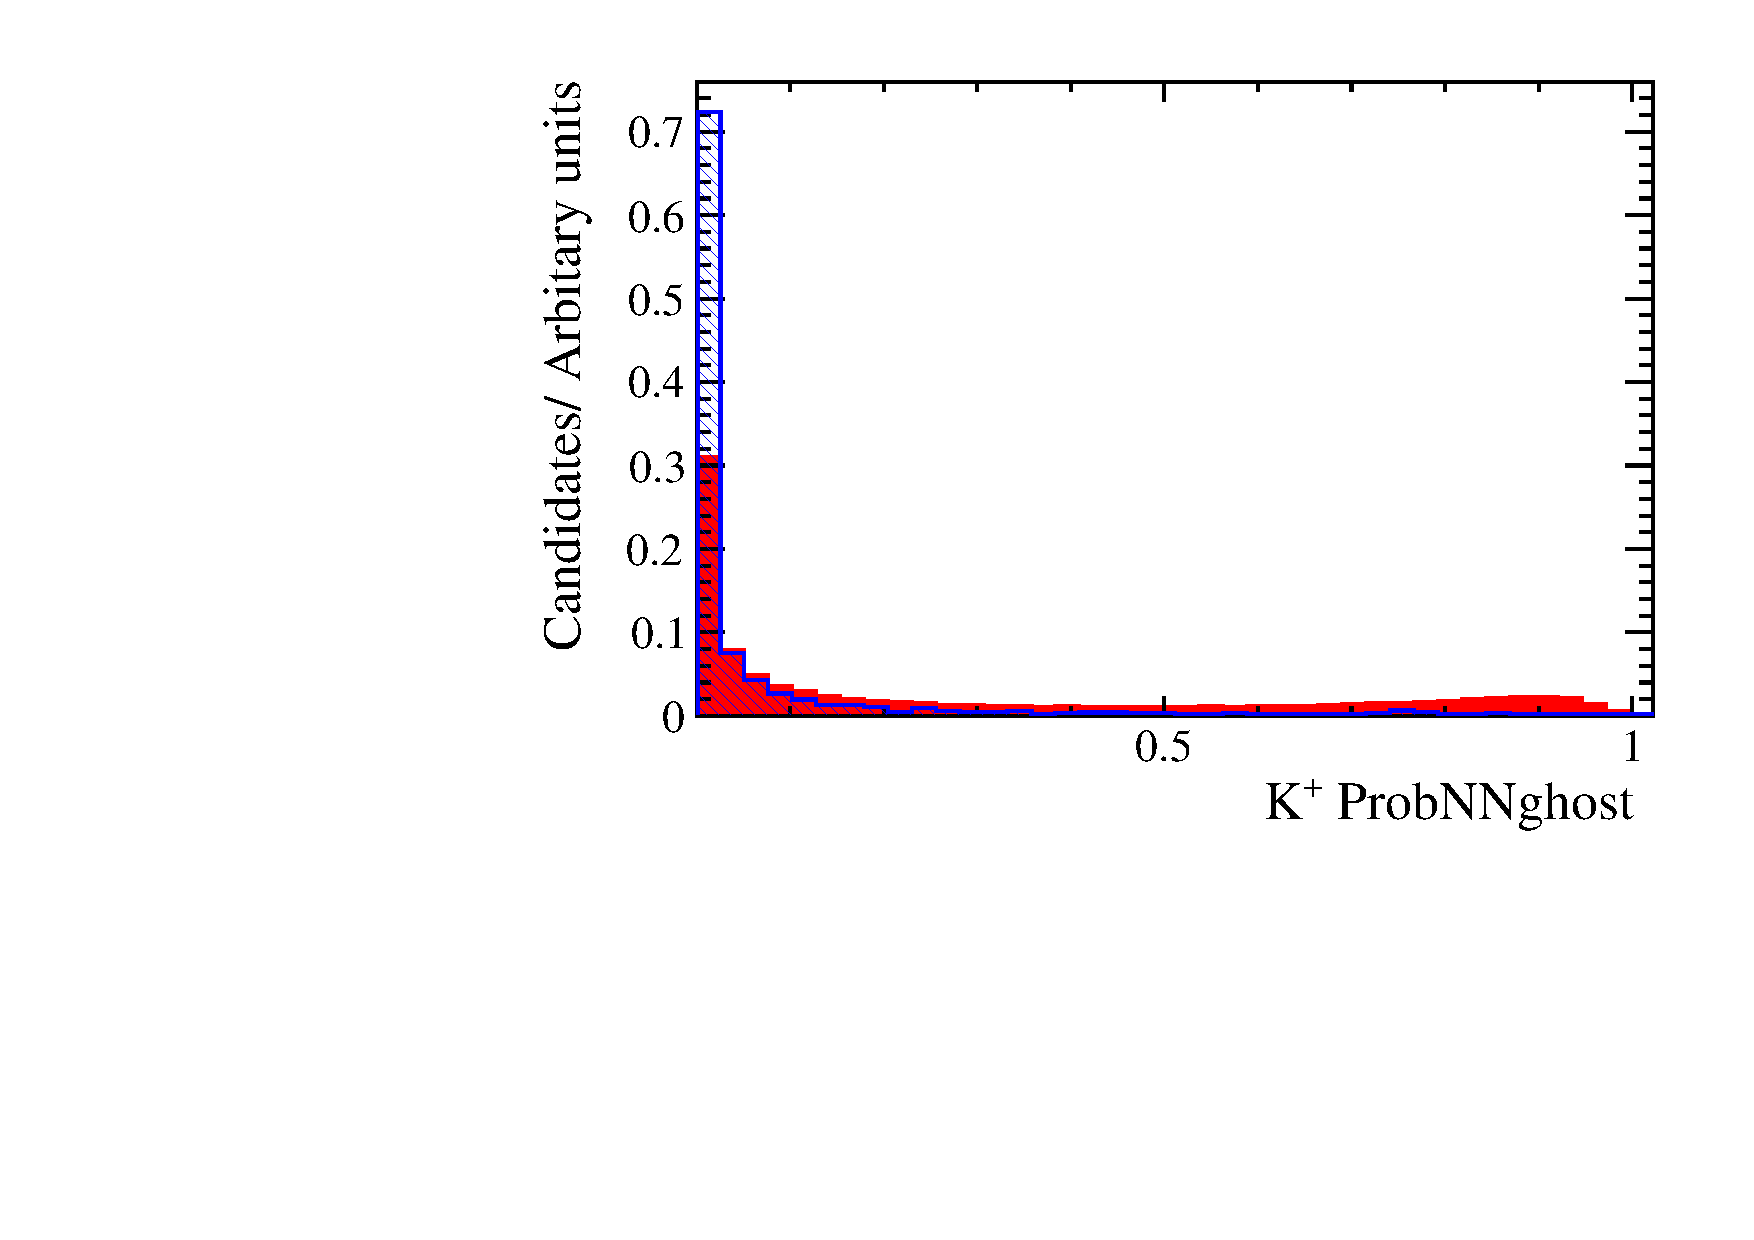
\includegraphics[width=1.0\textwidth]{figs/Selection/Phi_BDT_Var_Ds2KKPi_Phi_K0_MC15TuneV1_ProbNNghost.pdf}
   \end{subfigure}
   \begin{subfigure}[t]{0.22\textwidth}
      \centering
      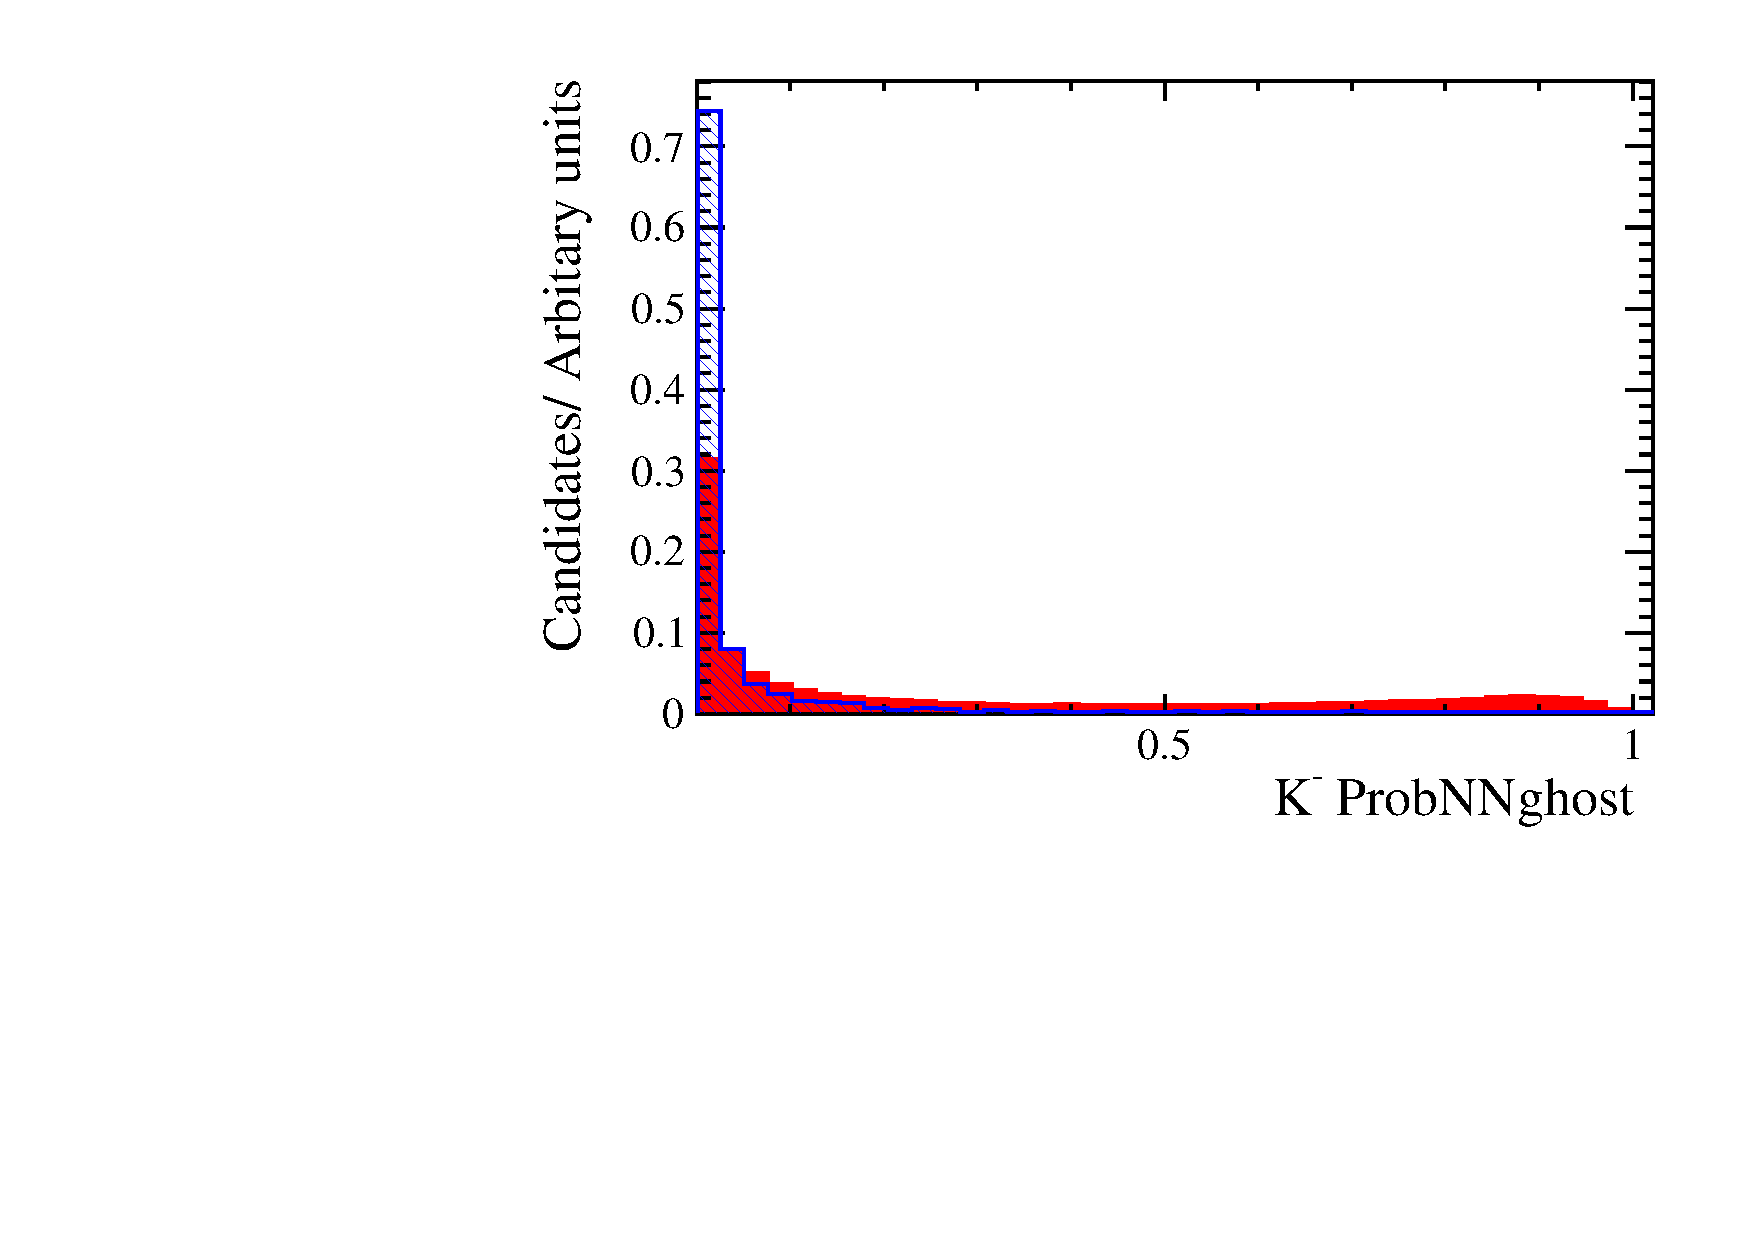
\includegraphics[width=1.0\textwidth]{figs/Selection/Phi_BDT_Var_Ds2KKPi_Phi_K1_MC15TuneV1_ProbNNghost.pdf}
   \end{subfigure}
   \begin{subfigure}[t]{0.22\textwidth}
      \centering
      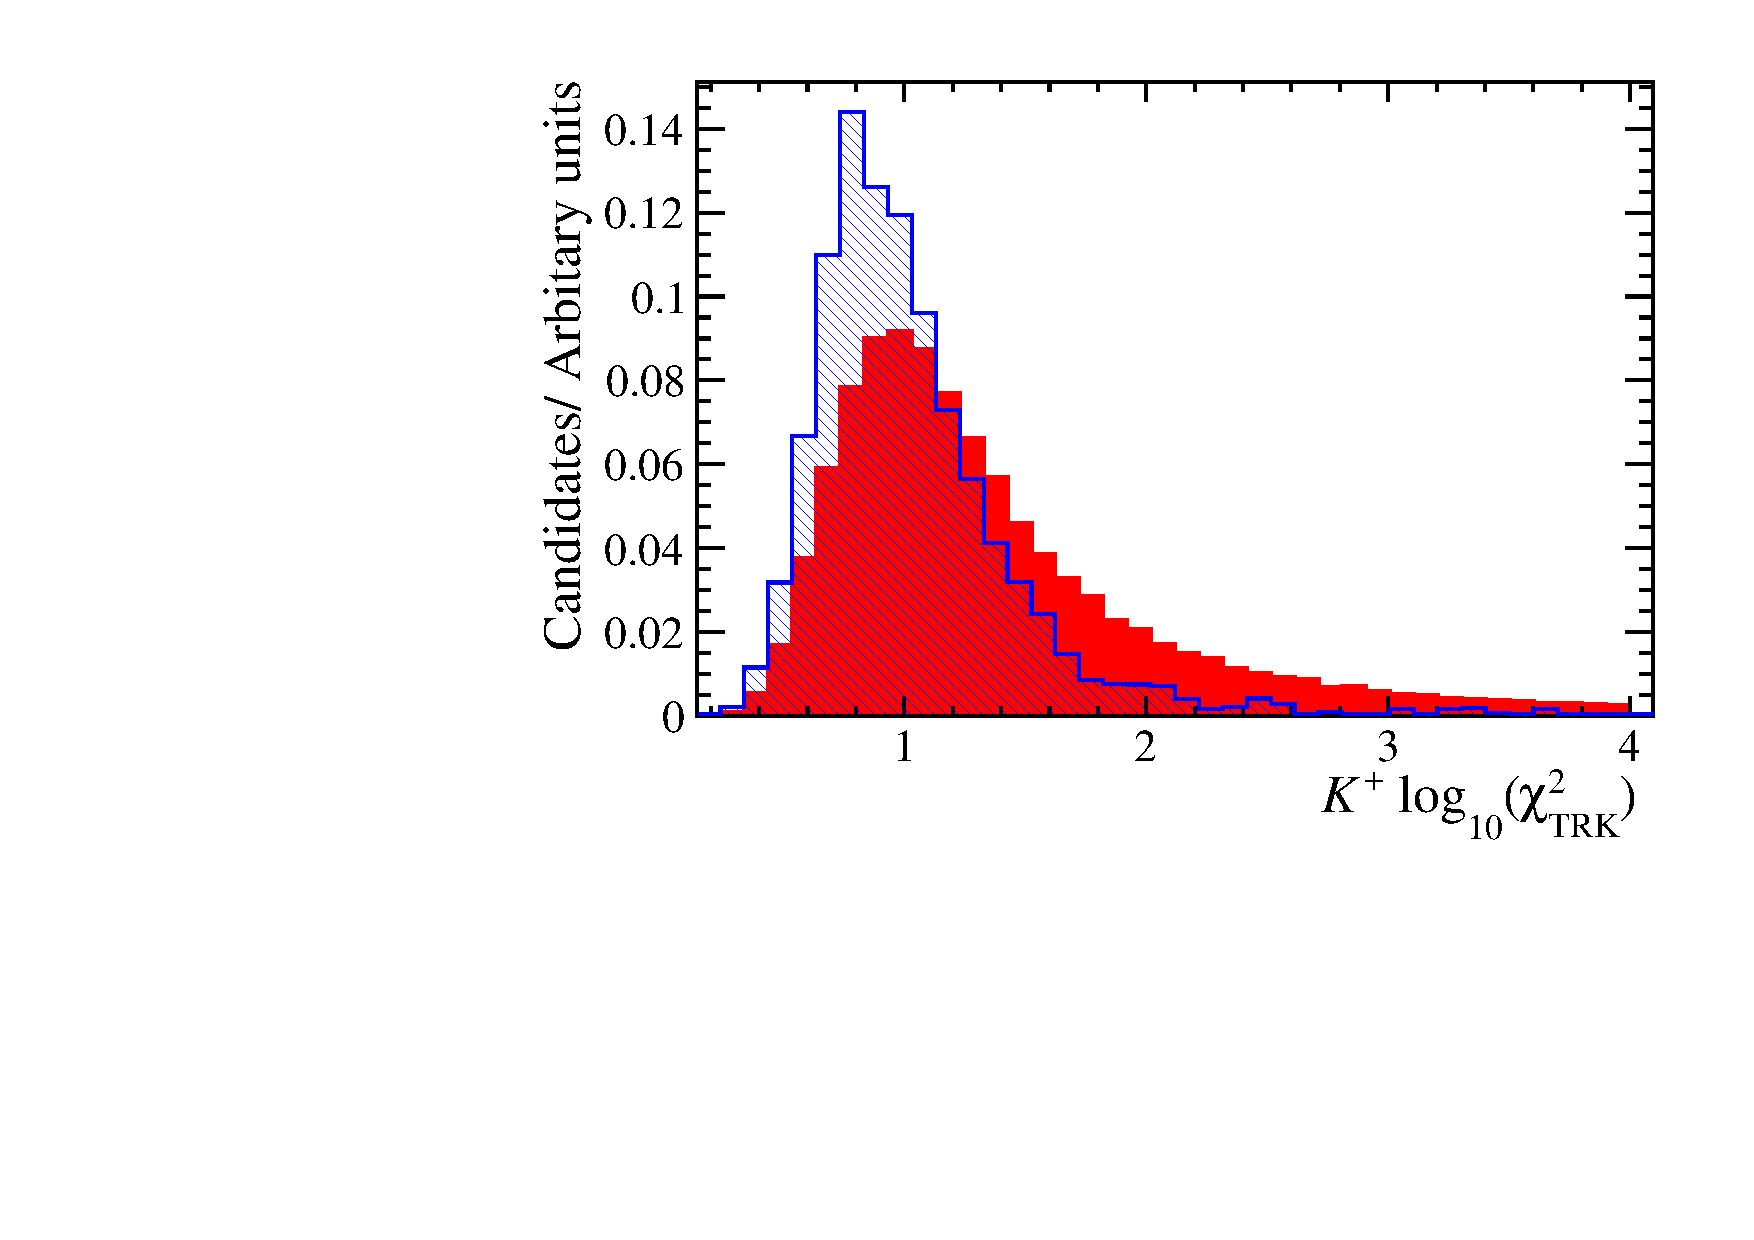
\includegraphics[width=1.0\textwidth]{figs/Selection/Phi_BDT_Var_Ds2KKPi_Phi_K0_TRACK_CHI2NDOF.pdf}
   \end{subfigure}
   \begin{subfigure}[t]{0.22\textwidth}
      \centering
      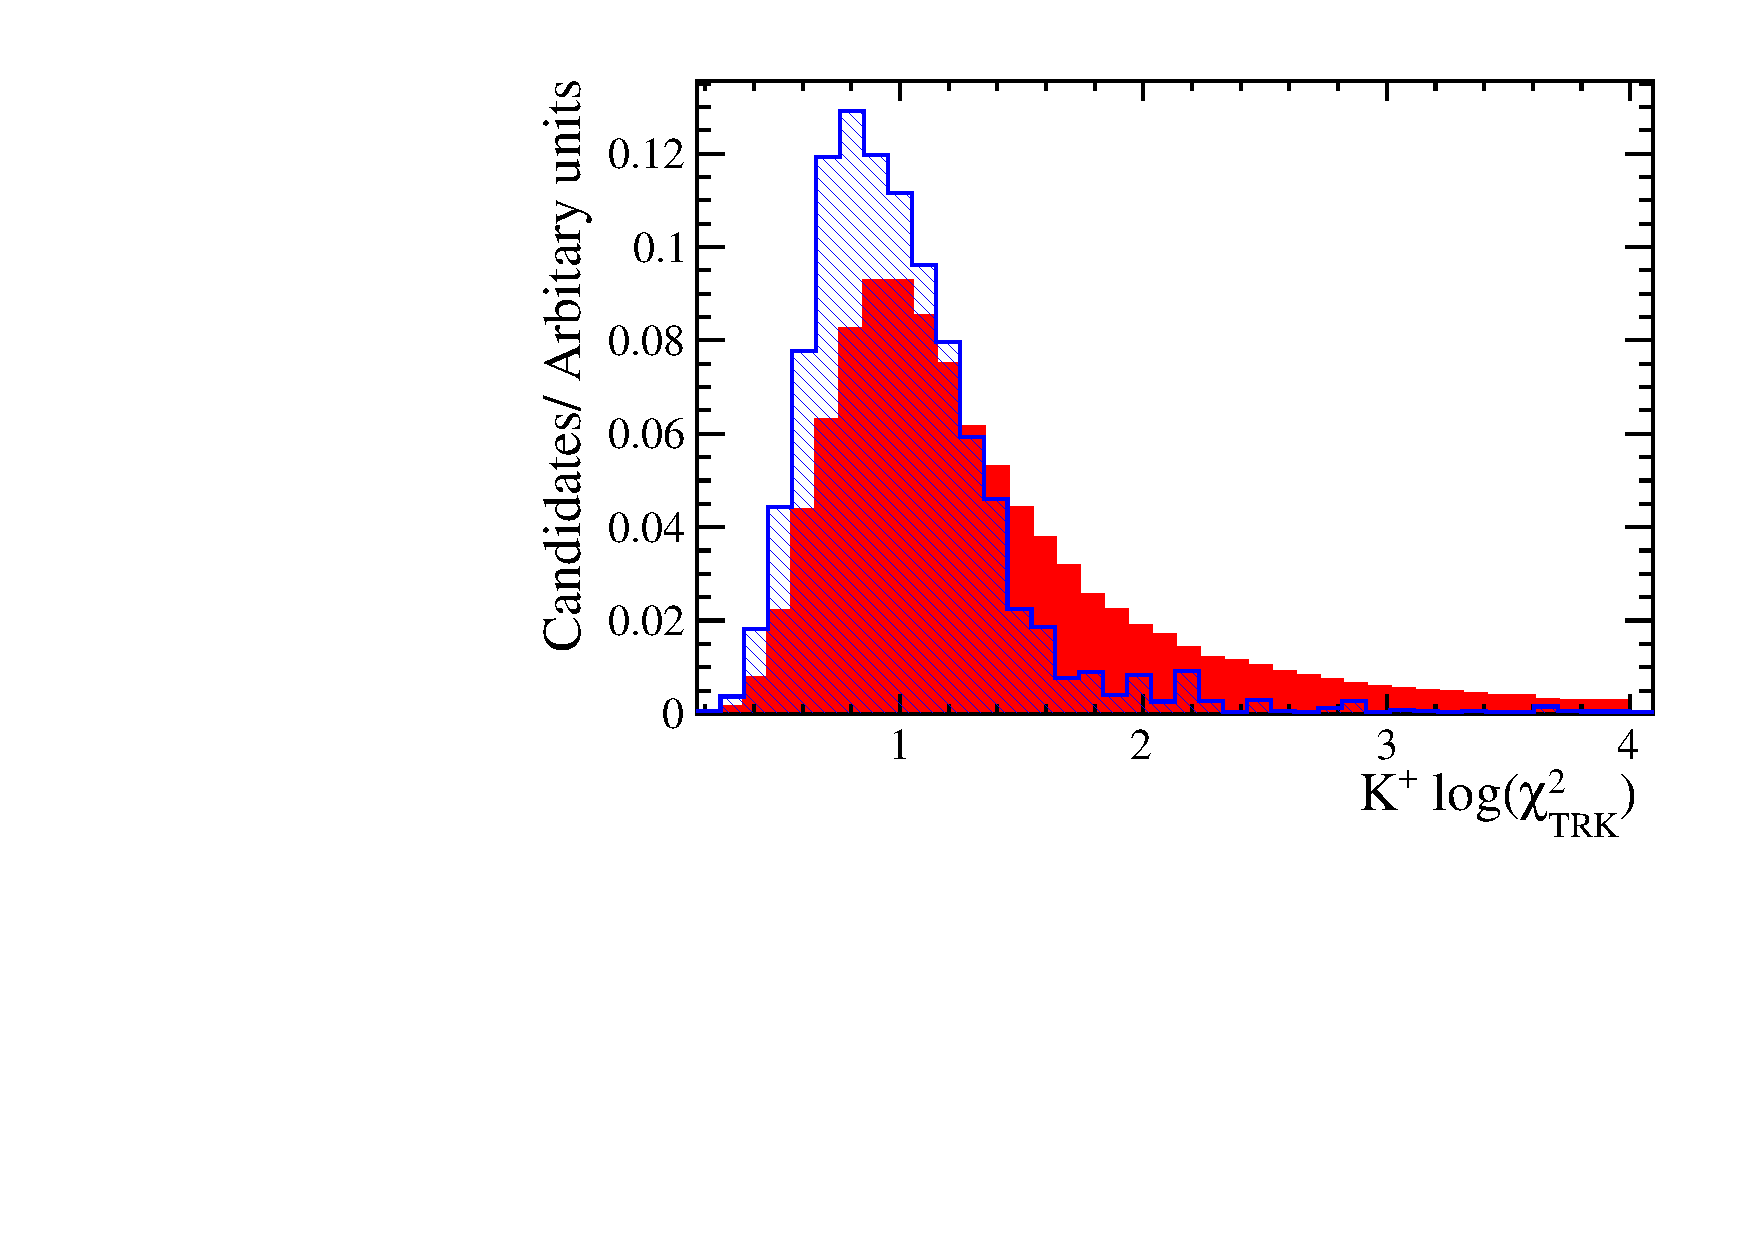
\includegraphics[width=1.0\textwidth]{figs/Selection/Phi_BDT_Var_Ds2KKPi_Phi_K1_TRACK_CHI2NDOF.pdf}
   \end{subfigure}
   \begin{subfigure}[t]{0.22\textwidth}
      \centering
      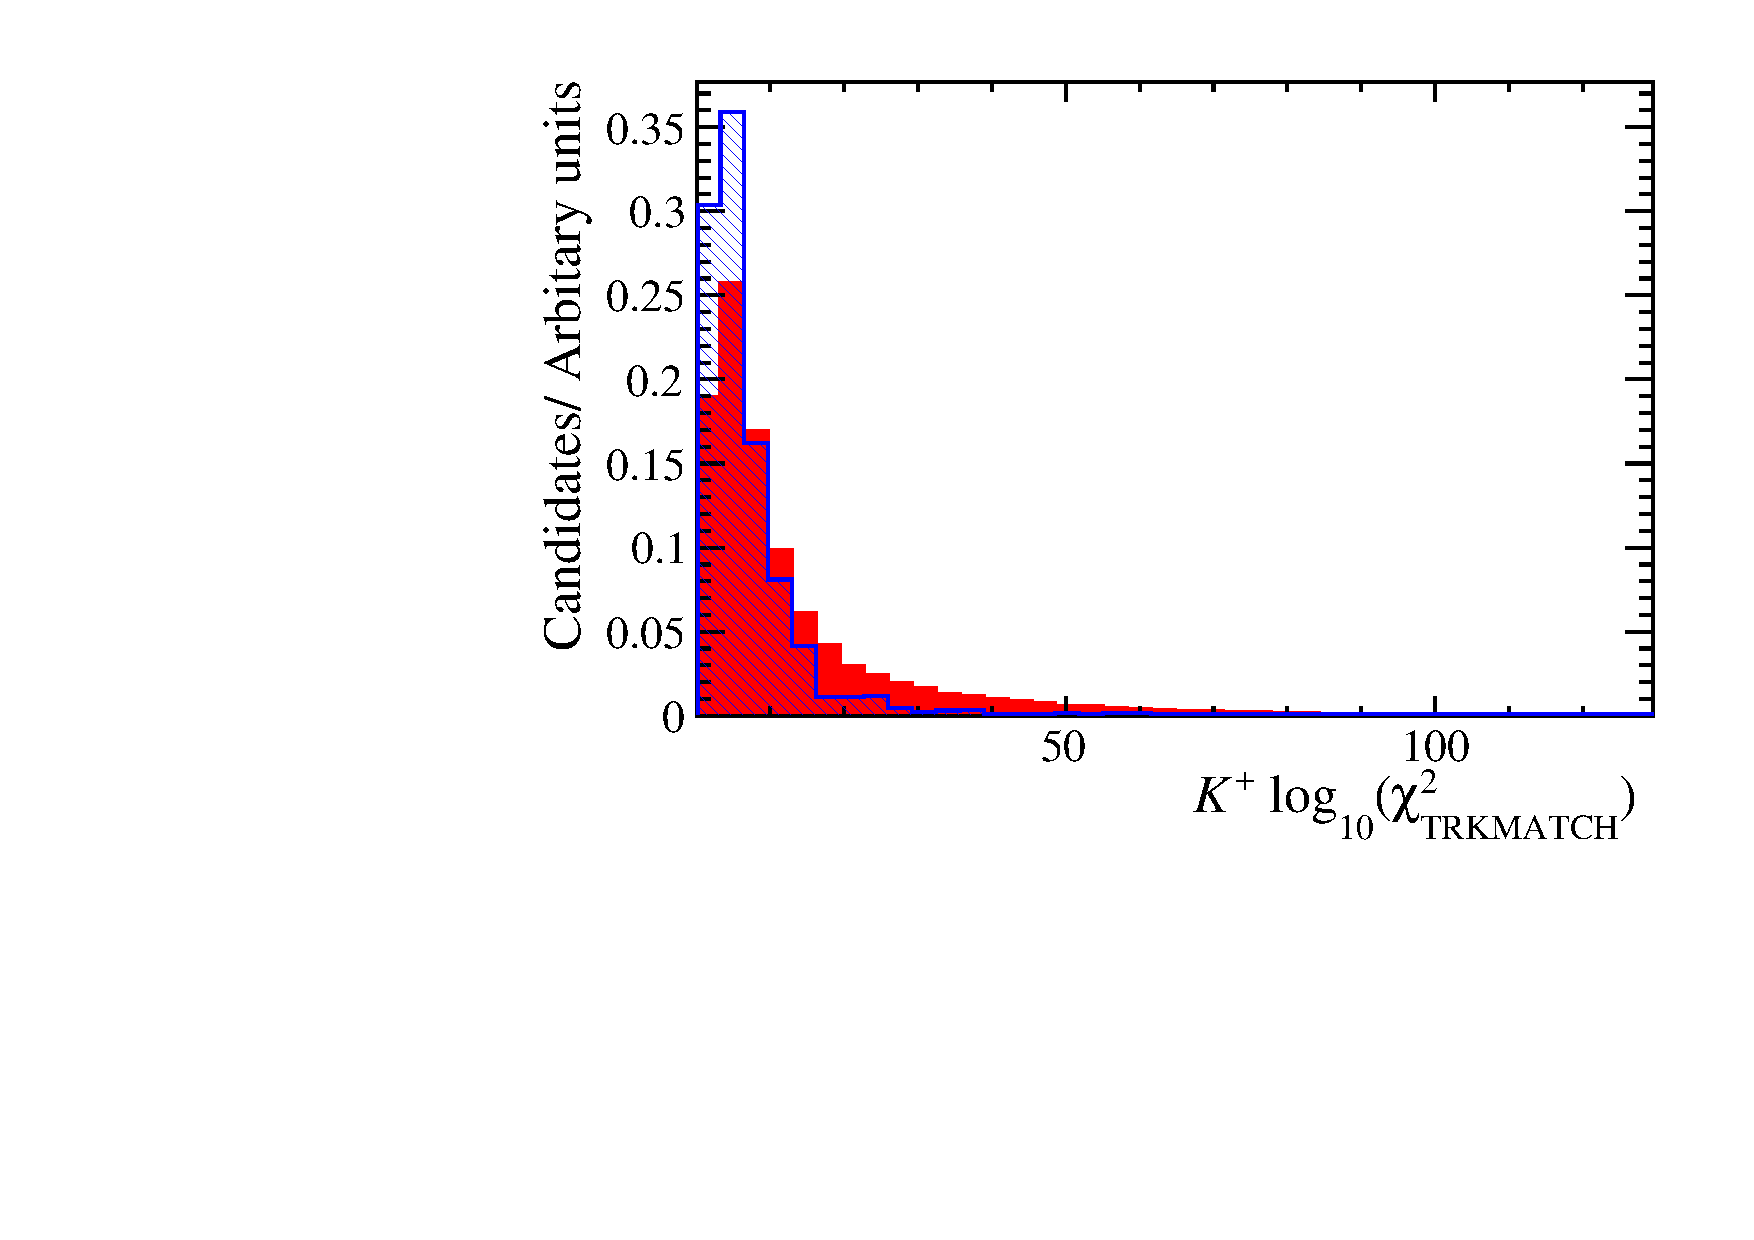
\includegraphics[width=1.0\textwidth]{figs/Selection/Phi_BDT_Var_Ds2KKPi_Phi_K0_TRACK_MatchCHI2.pdf}
   \end{subfigure}
   \begin{subfigure}[t]{0.22\textwidth}
      \centering
      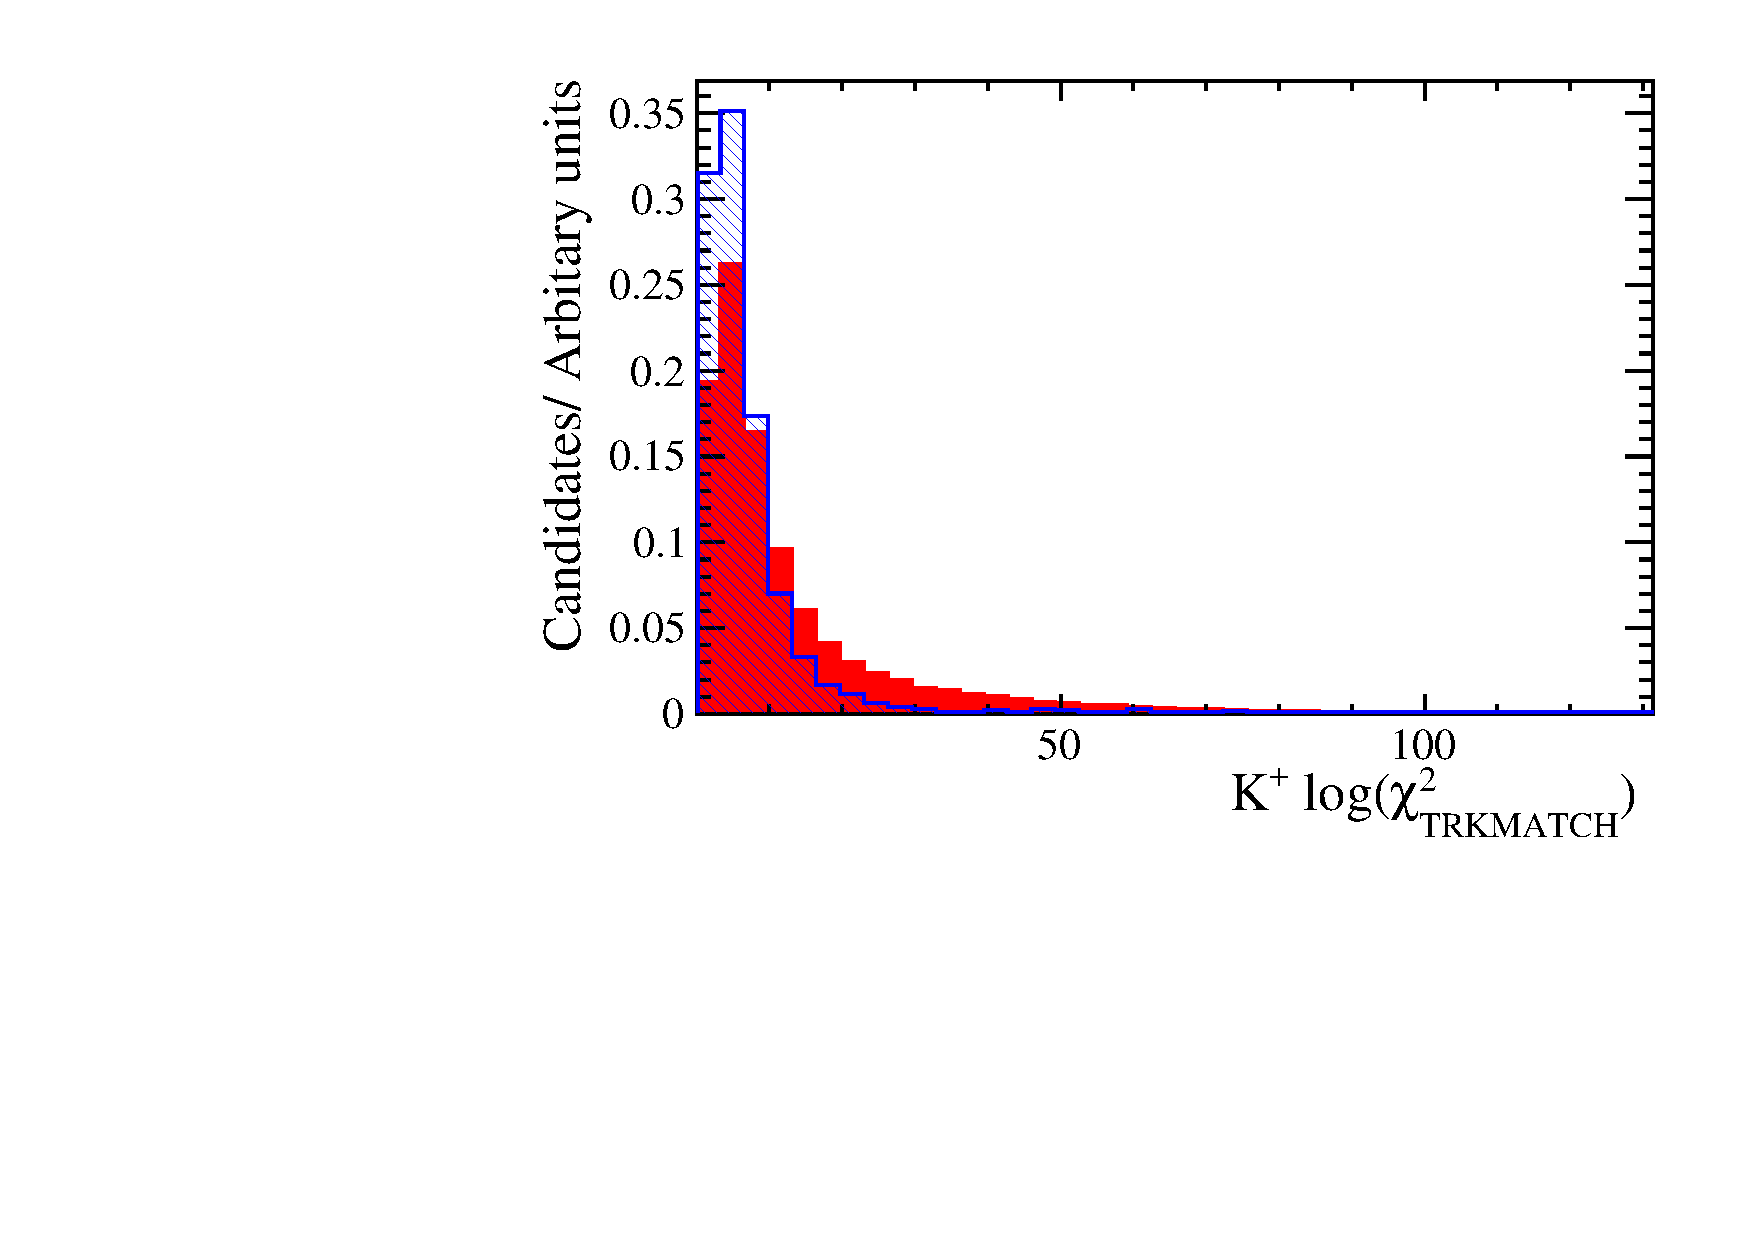
\includegraphics[width=1.0\textwidth]{figs/Selection/Phi_BDT_Var_Ds2KKPi_Phi_K1_TRACK_MatchCHI2.pdf}
   \end{subfigure}
   \caption{Distributions of MVA training variables in the signal (blue) and background (red) samples for the Run~II \decay{\phiz}{\Kp\Km} MVA.}
   \label{fig:mvatrainingvariables_phi}   
\end{figure}
%%%%%%%%%%%%%%%%%%%%%%%%%%%%%%%%%%%%%%%%%%%%%%%%%%%%%%%%%%



%%%%%%%%%%%%%%%%%%%%%%%%%%%%%%%%%%%%%%%%%%%%%%%%%%%%%%%%%%
\begin{figure}[!h]
   \centering
   \begin{subfigure}[t]{0.22\textwidth}
      \centering
      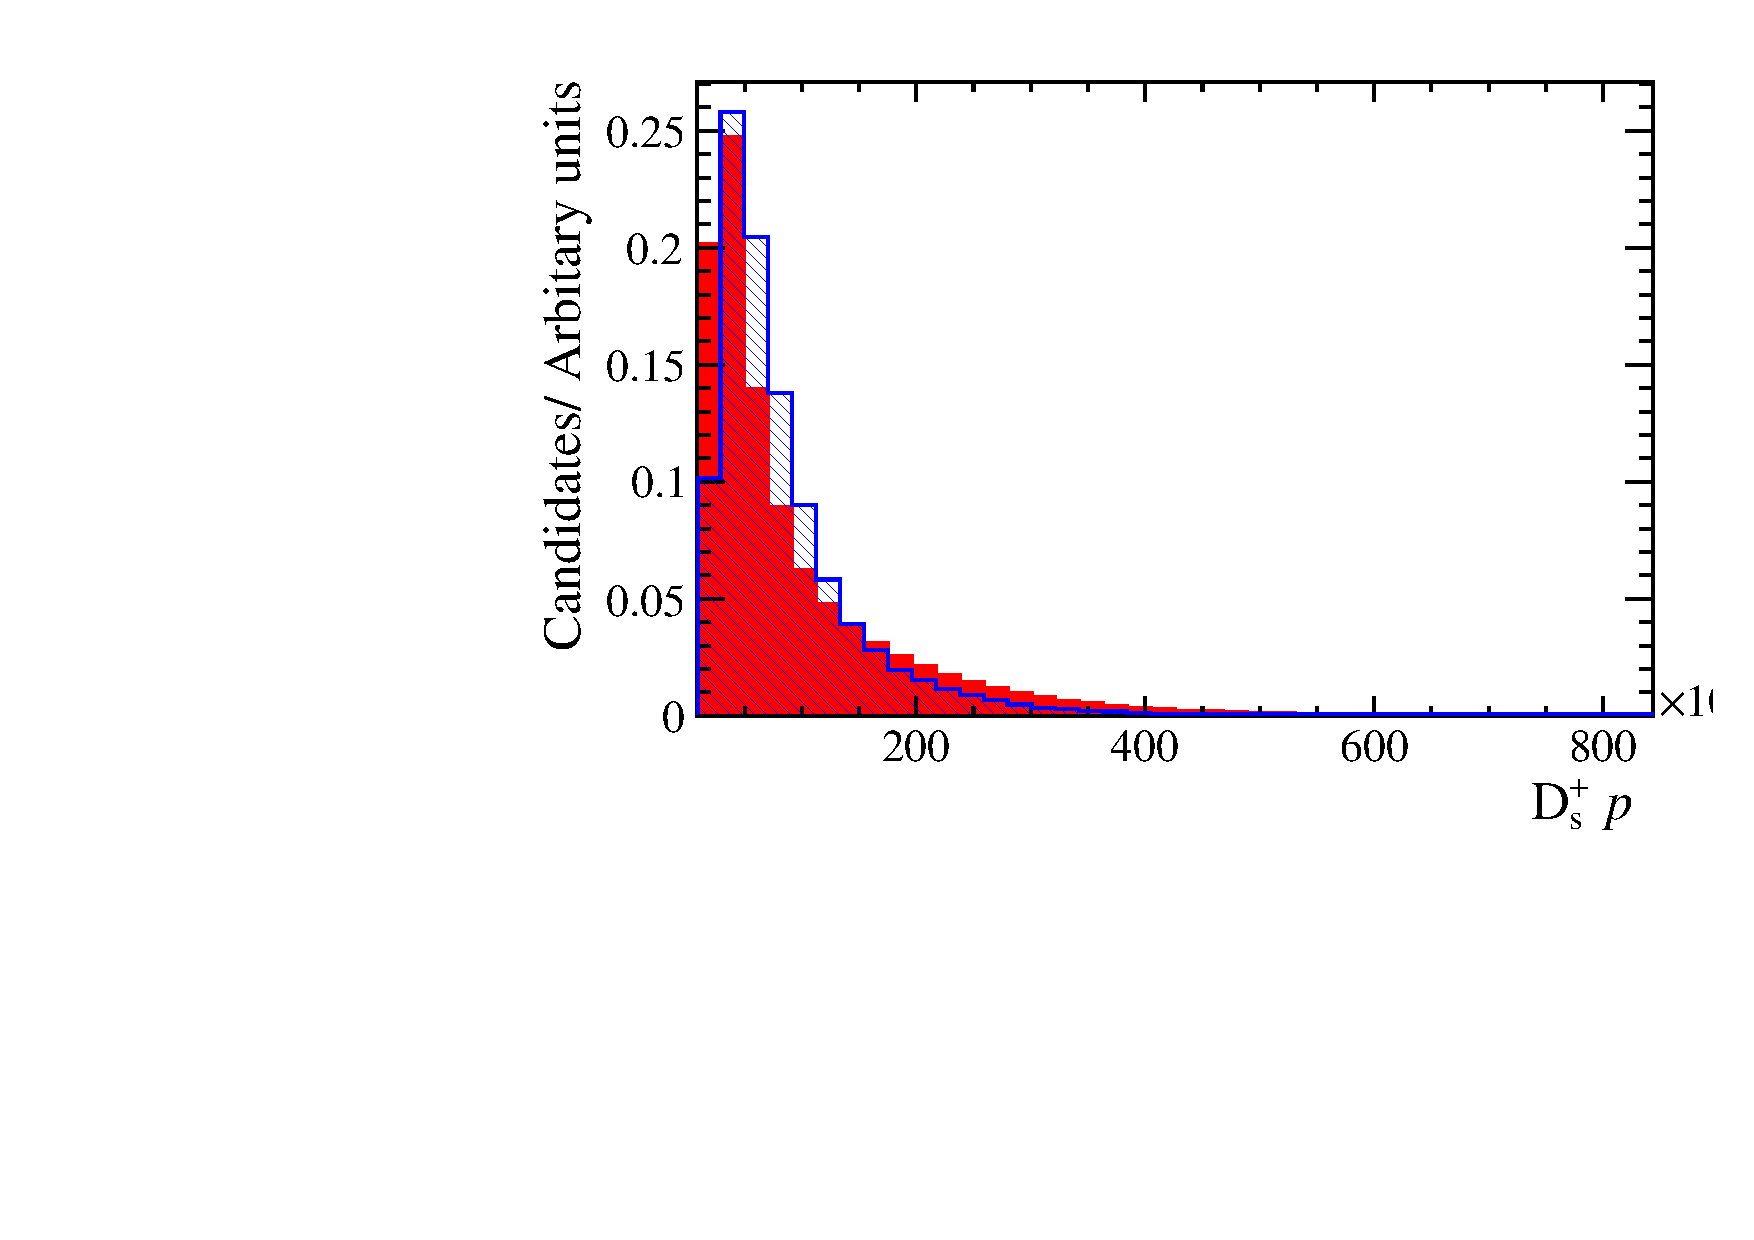
\includegraphics[width=1.0\textwidth]{figs/Selection/Ds_BDT_Var_Ds2KKPi_D_P.pdf}
   \end{subfigure}
   \begin{subfigure}[t]{0.22\textwidth}
      \centering
      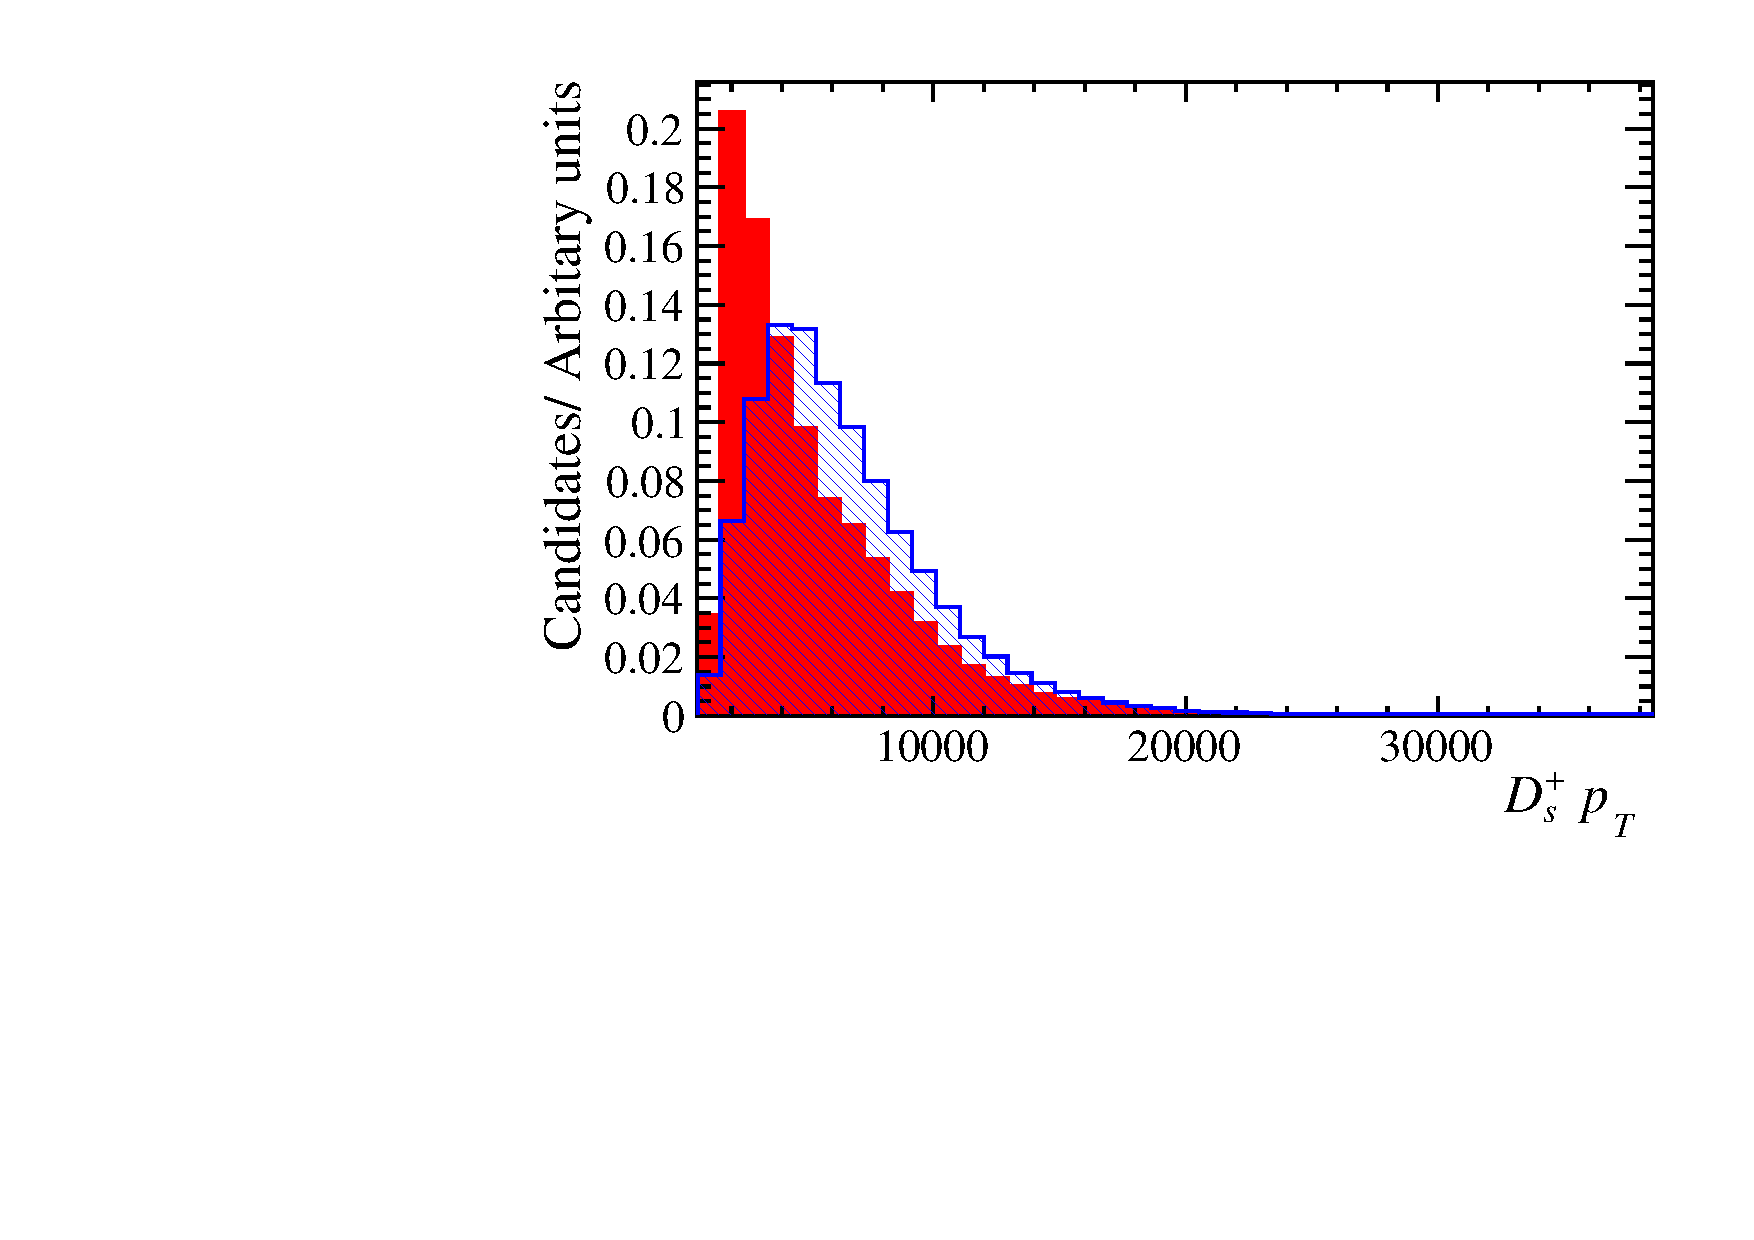
\includegraphics[width=1.0\textwidth]{figs/Selection/Ds_BDT_Var_Ds2KKPi_D_PT.pdf}
   \end{subfigure}
   \begin{subfigure}[t]{0.22\textwidth}
      \centering
      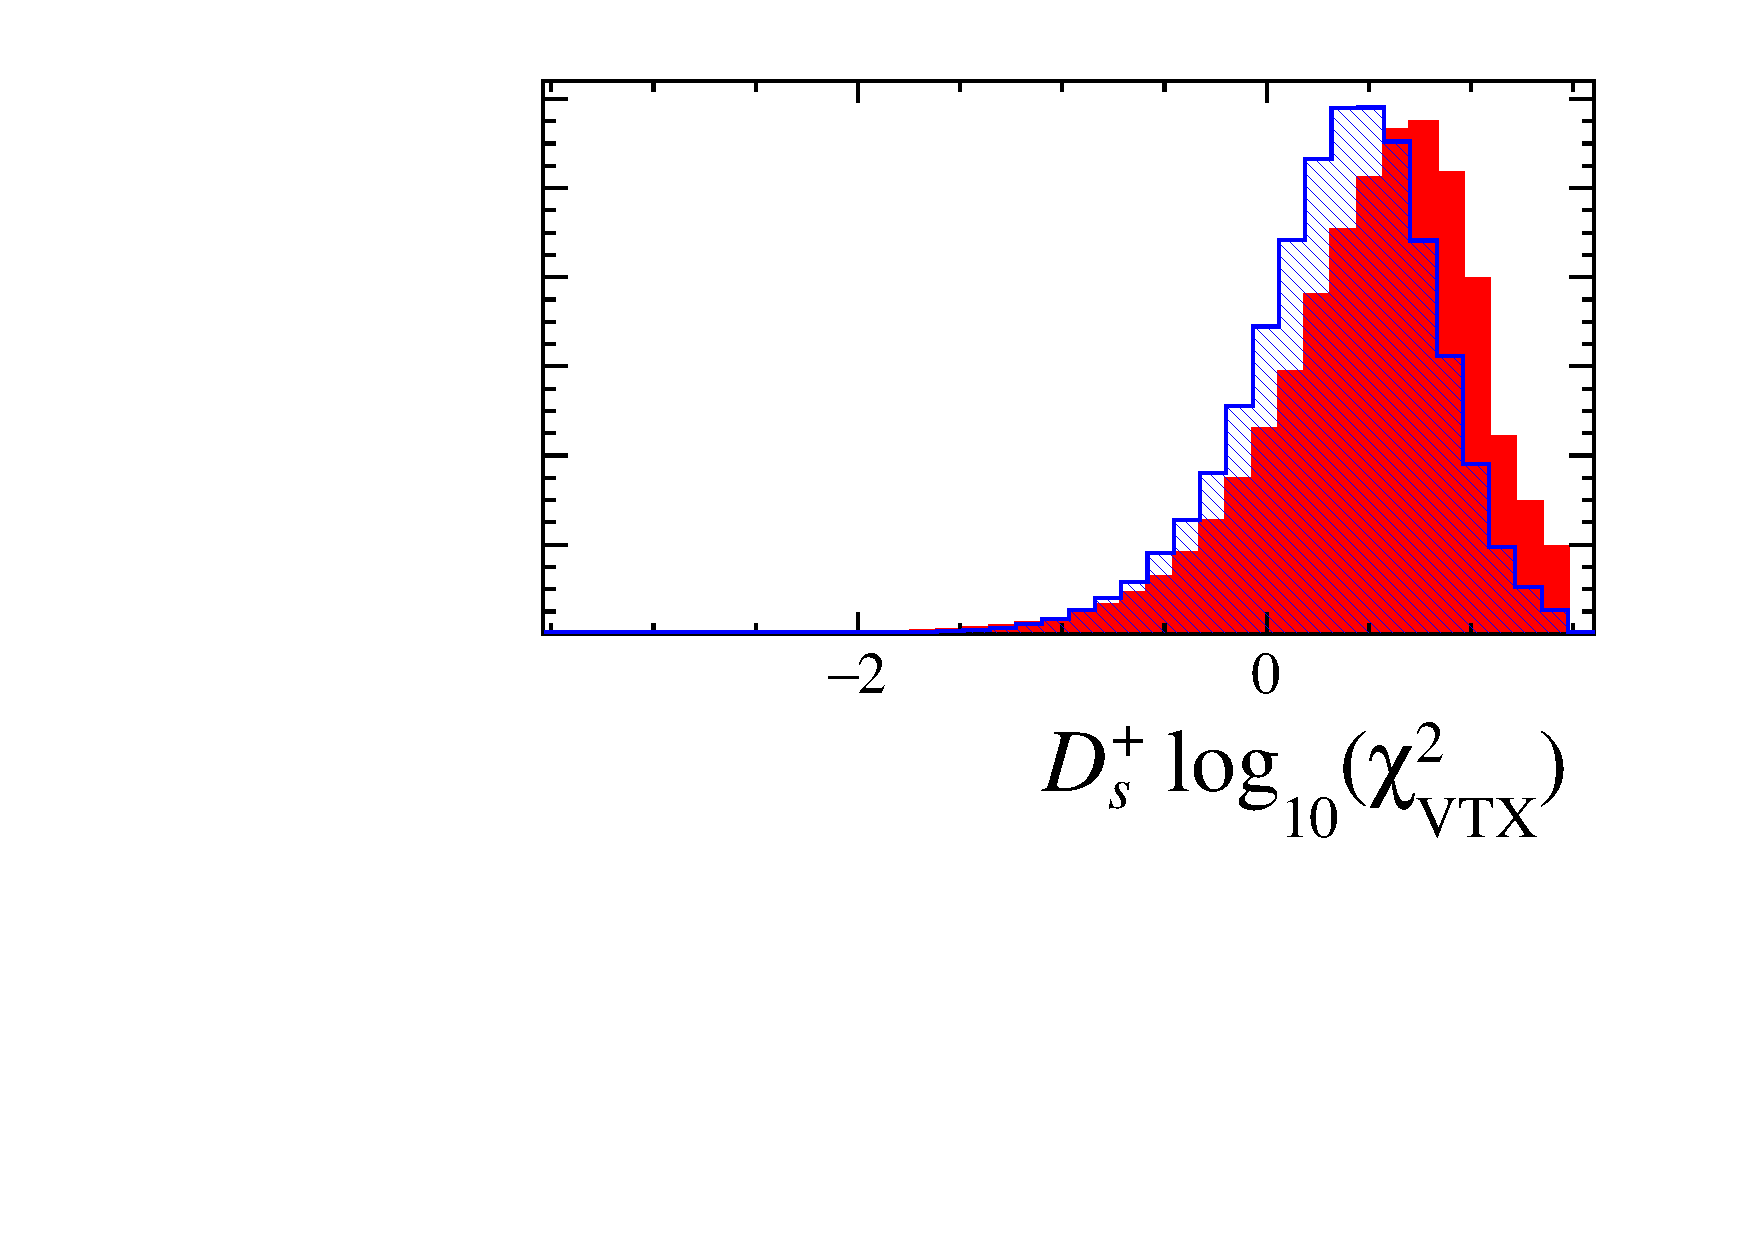
\includegraphics[width=1.0\textwidth]{figs/Selection/Ds_BDT_Var_Ds2KKPi_log10_D_ENDVERTEX_CHI2.pdf}
   \end{subfigure}
   \begin{subfigure}[t]{0.22\textwidth}
      \centering
      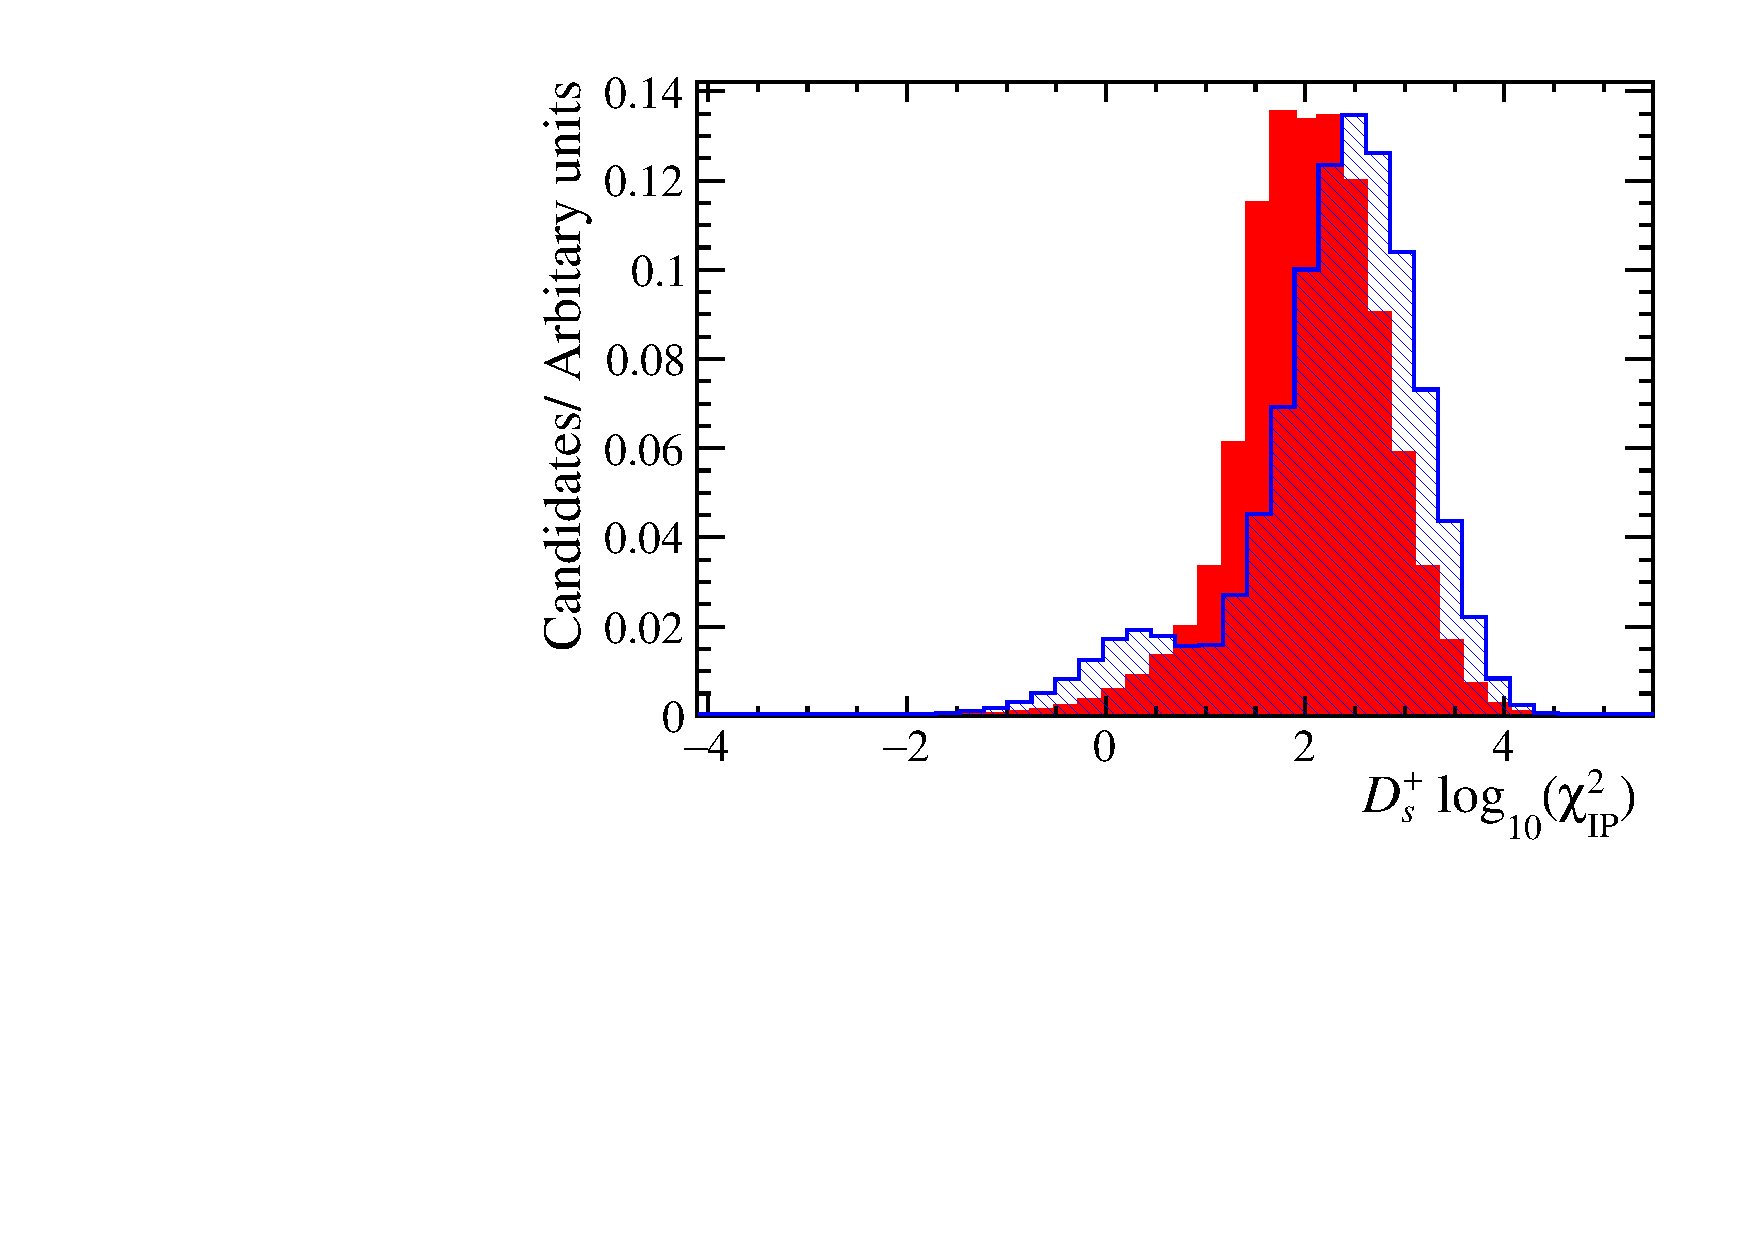
\includegraphics[width=1.0\textwidth]{figs/Selection/Ds_BDT_Var_Ds2KKPi_log10_D_IPCHI2_OWNPV.pdf}
   \end{subfigure}
   \begin{subfigure}[t]{0.22\textwidth}
      \centering
      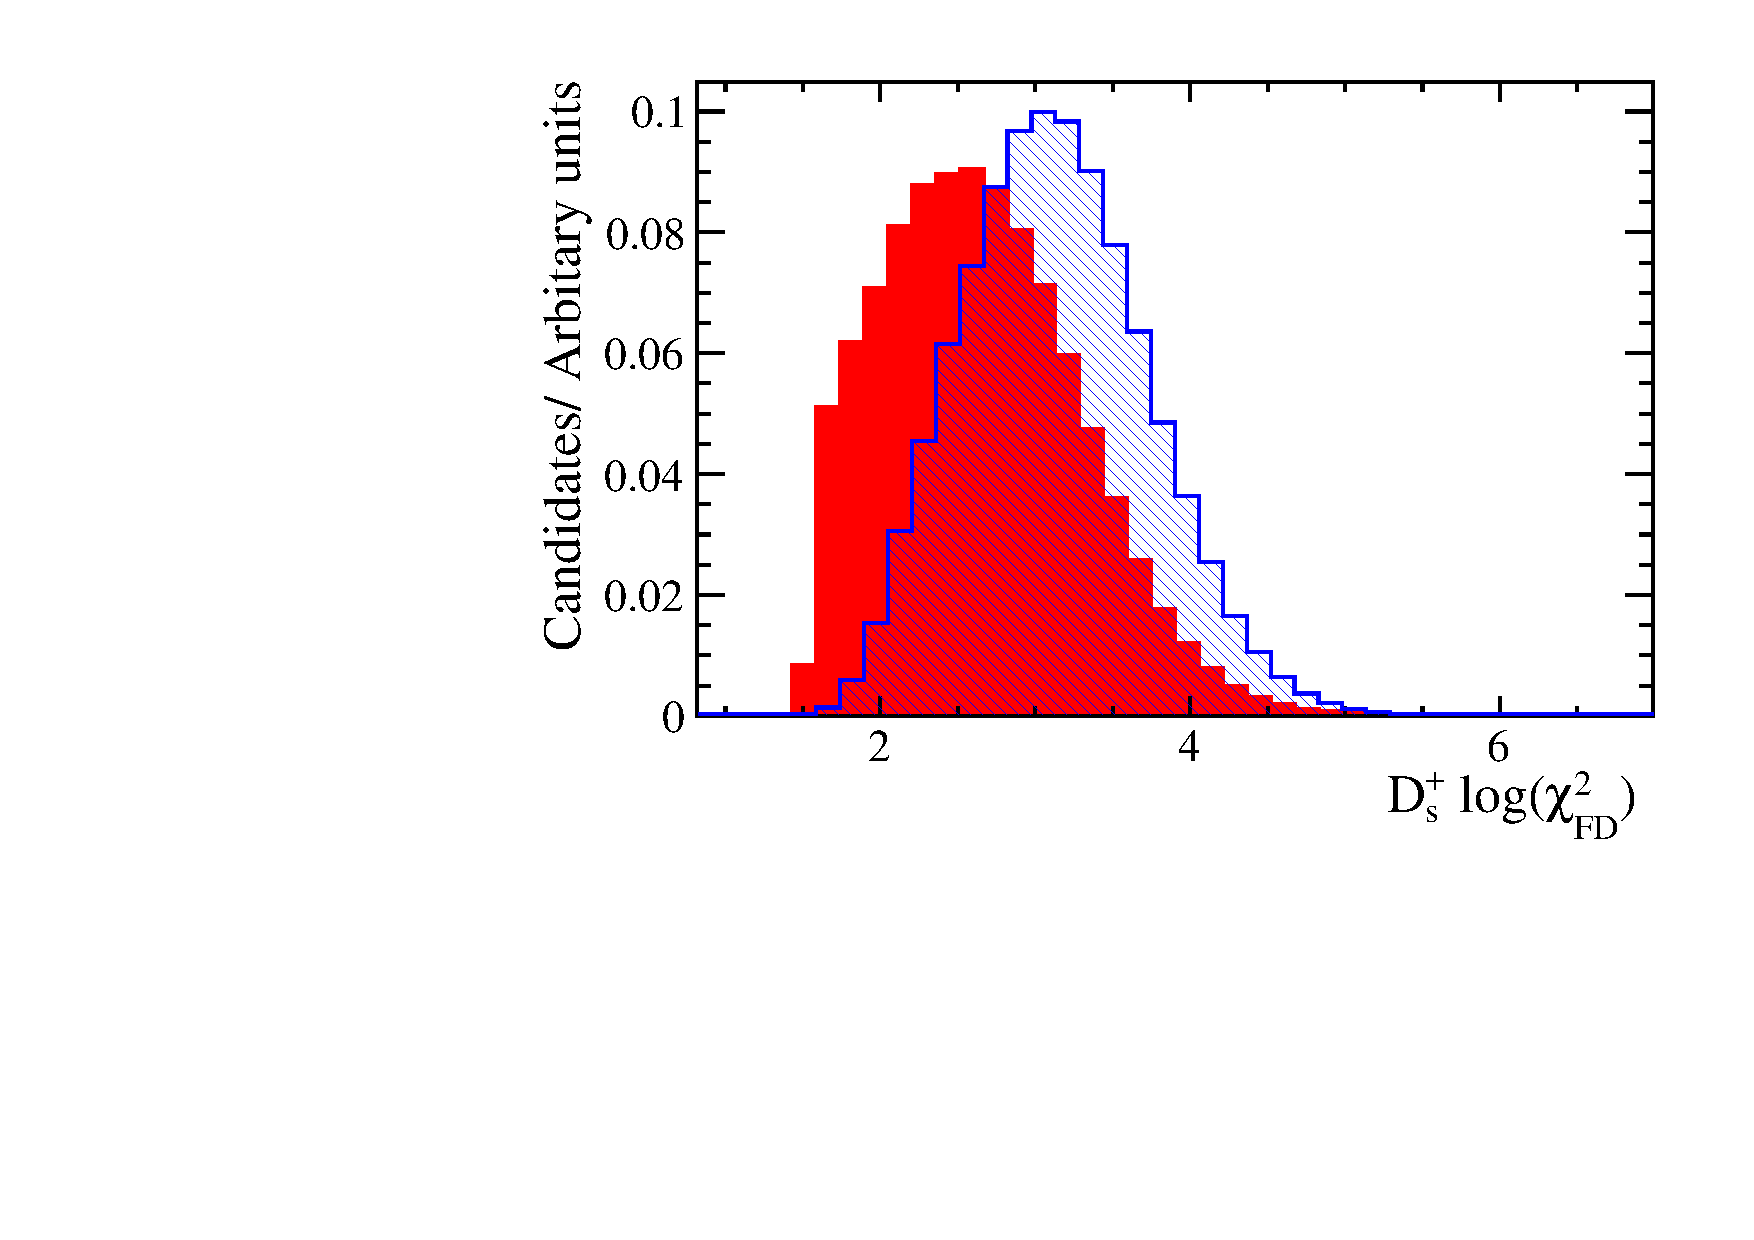
\includegraphics[width=1.0\textwidth]{figs/Selection/Ds_BDT_Var_Ds2KKPi_log10_D_FDCHI2_OWNPV.pdf}
   \end{subfigure}
   \begin{subfigure}[t]{0.22\textwidth}
      \centering
      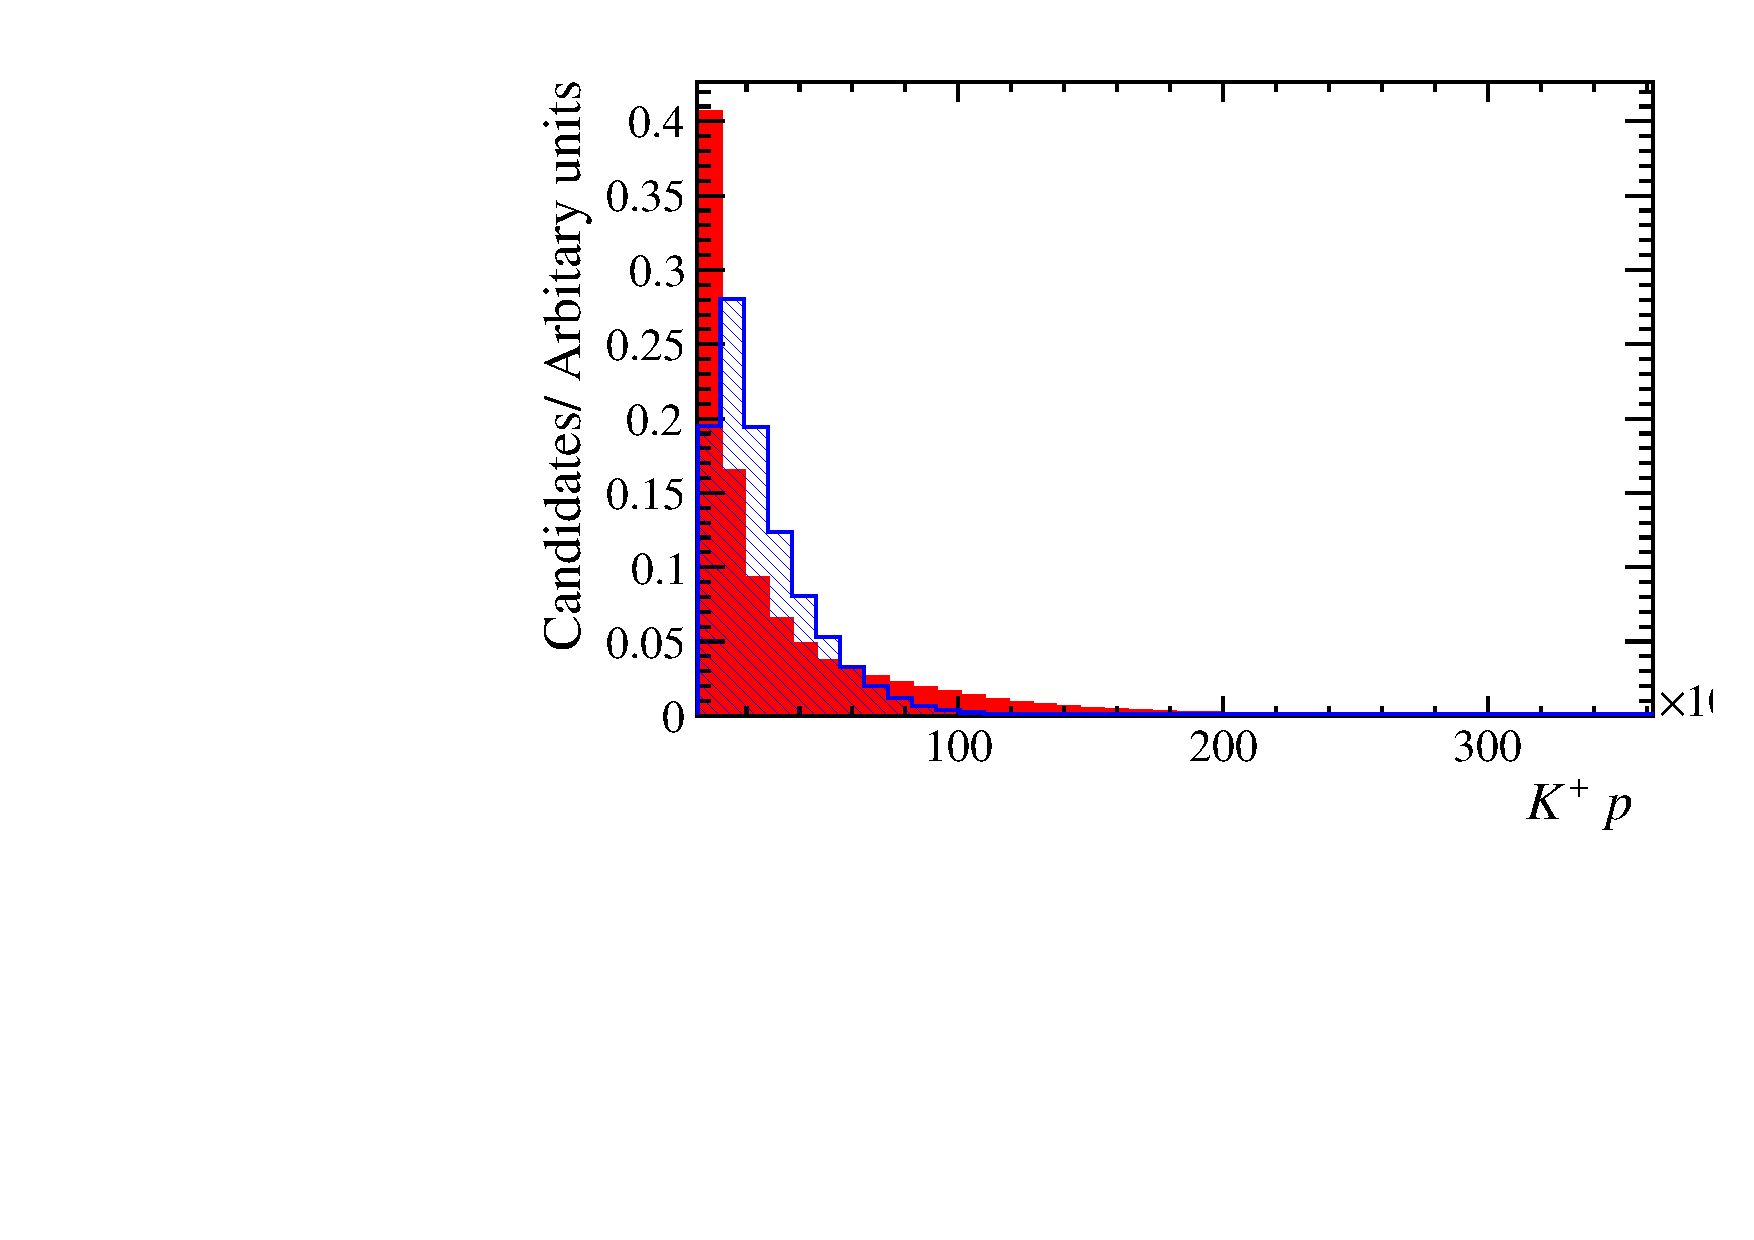
\includegraphics[width=1.0\textwidth]{figs/Selection/Ds_BDT_Var_Ds2KKPi_D_K0_P.pdf}
   \end{subfigure}
   \begin{subfigure}[t]{0.22\textwidth}
      \centering
      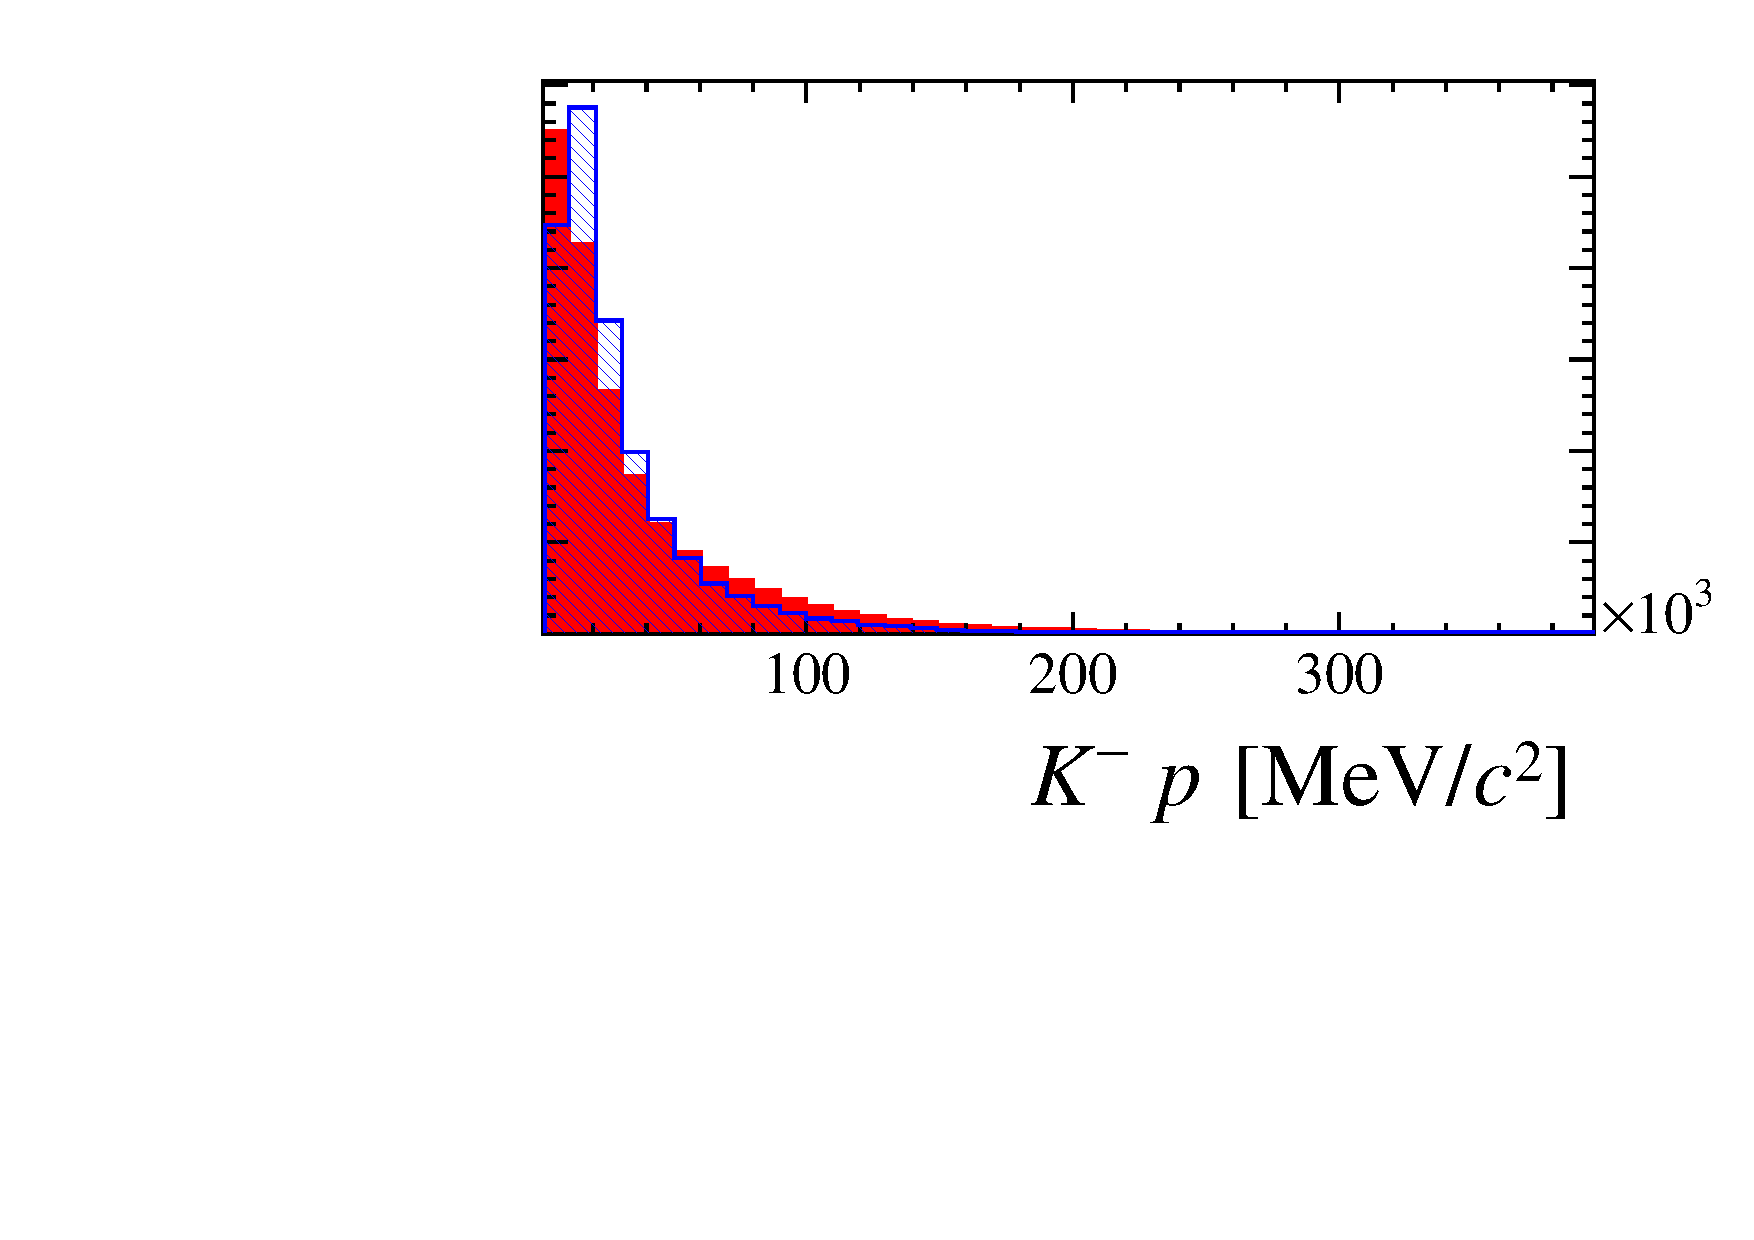
\includegraphics[width=1.0\textwidth]{figs/Selection/Ds_BDT_Var_Ds2KKPi_D_K1_P.pdf}
   \end{subfigure}
   \begin{subfigure}[t]{0.22\textwidth}
      \centering
      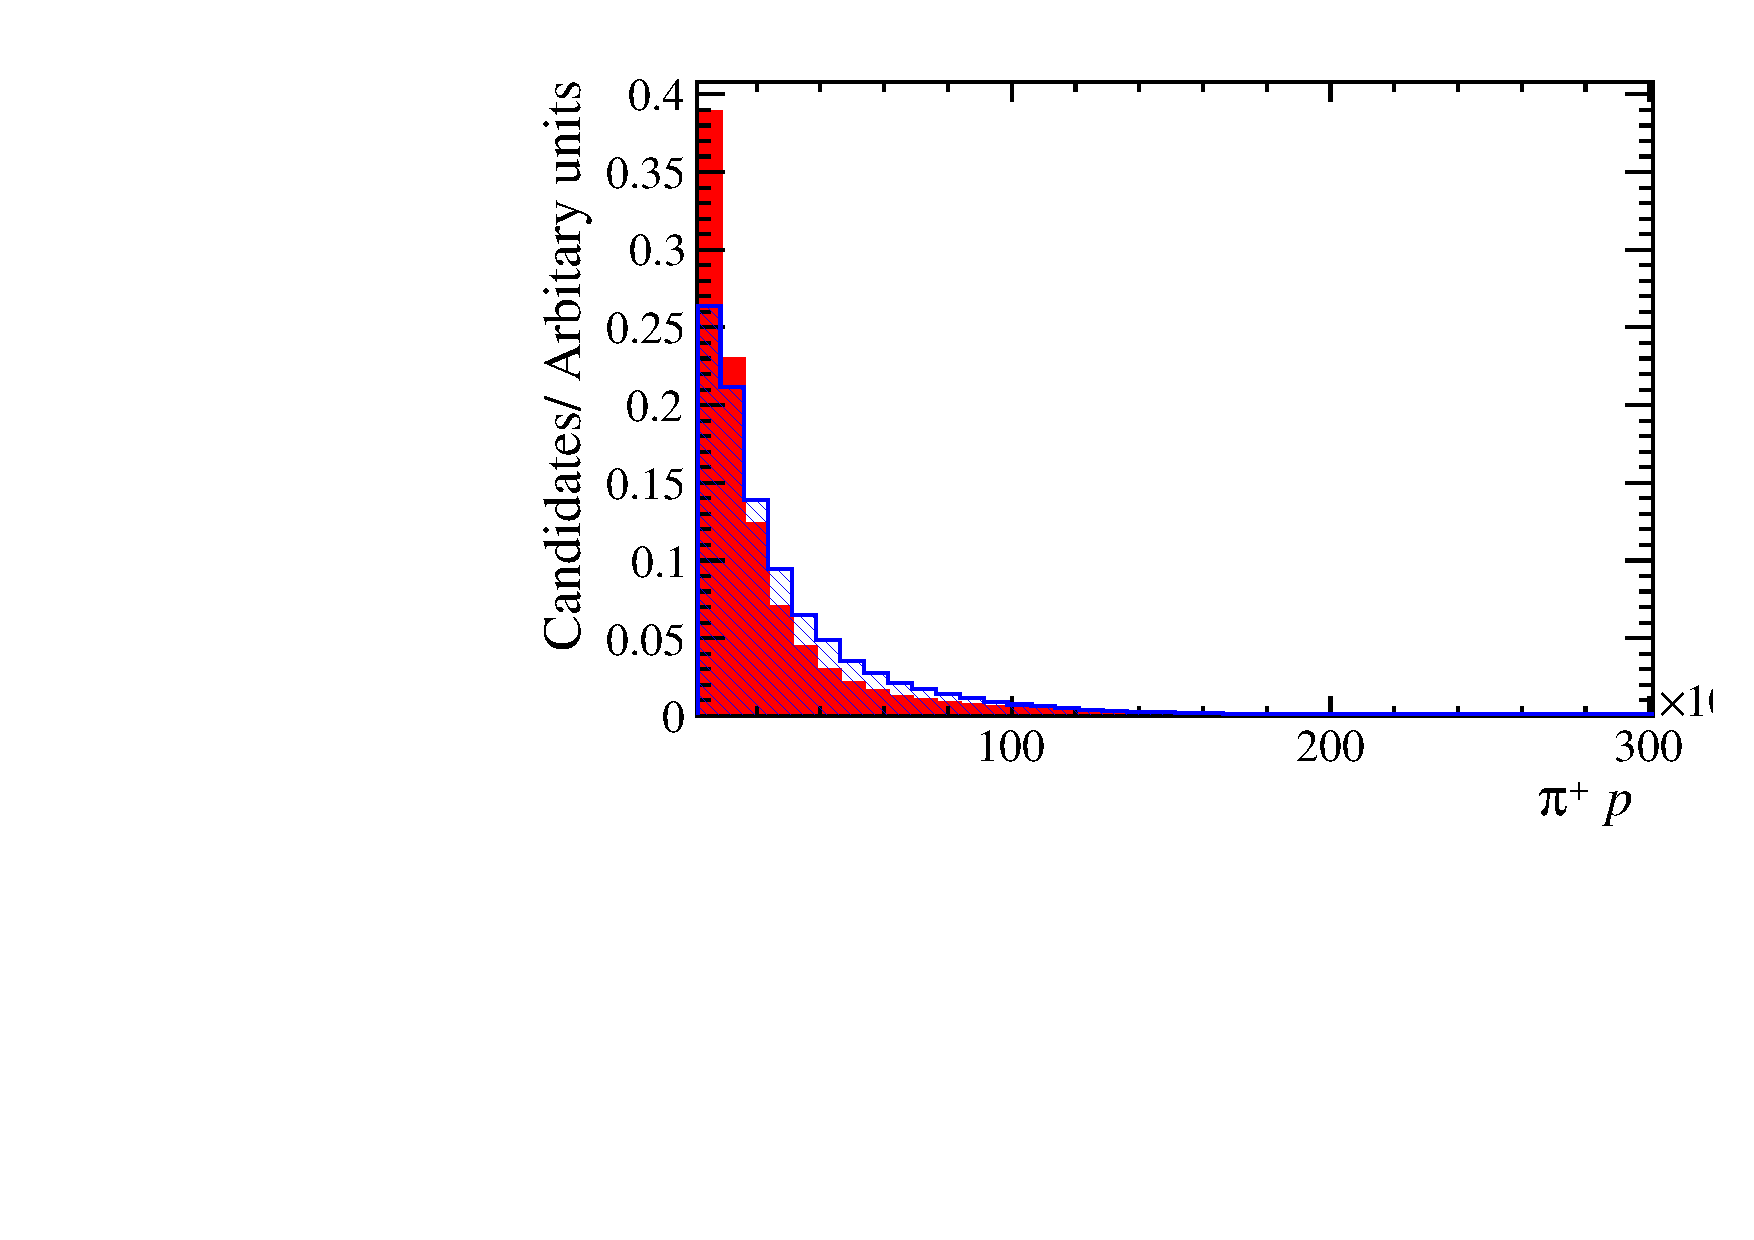
\includegraphics[width=1.0\textwidth]{figs/Selection/Ds_BDT_Var_Ds2KKPi_D_P_P.pdf}
   \end{subfigure}
   \begin{subfigure}[t]{0.22\textwidth}
      \centering
      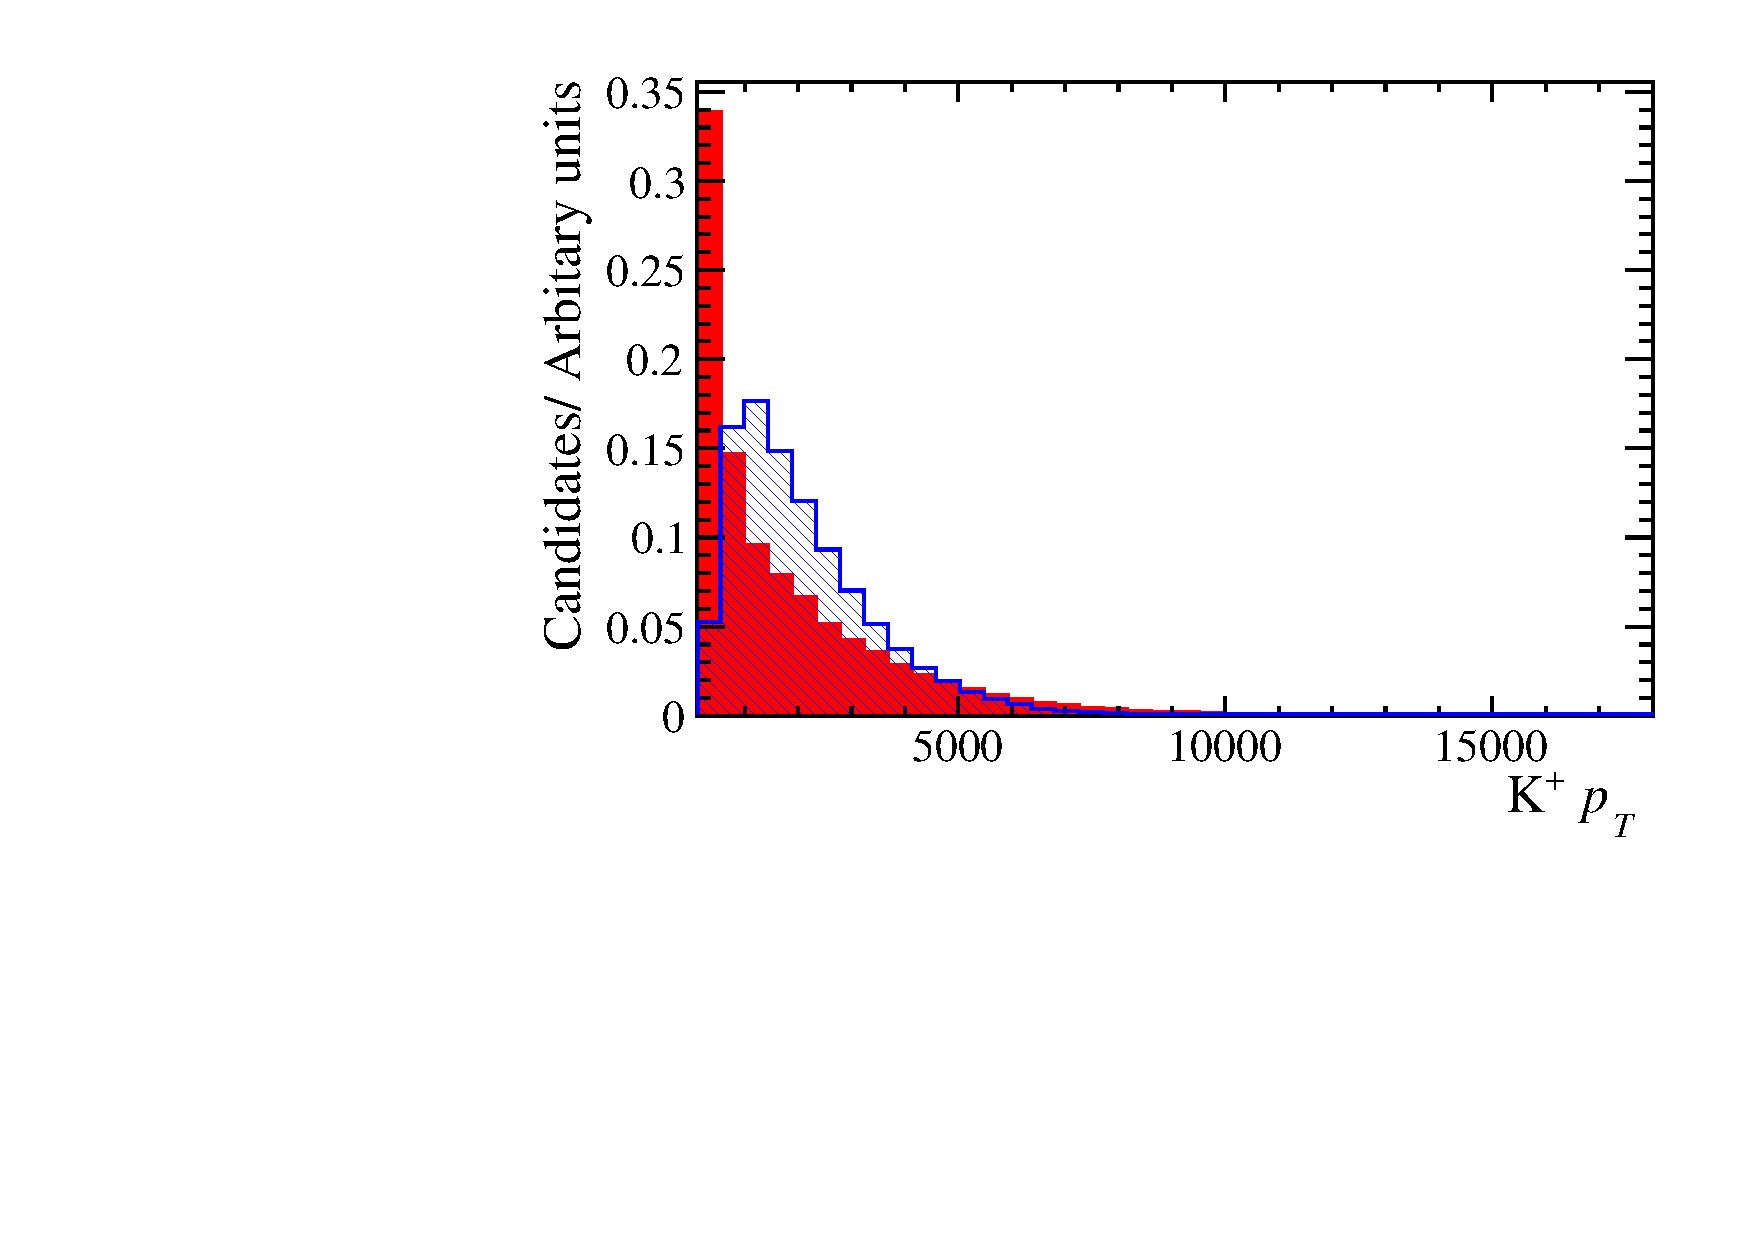
\includegraphics[width=1.0\textwidth]{figs/Selection/Ds_BDT_Var_Ds2KKPi_D_K0_PT.pdf}
   \end{subfigure}
   \begin{subfigure}[t]{0.22\textwidth}
      \centering
      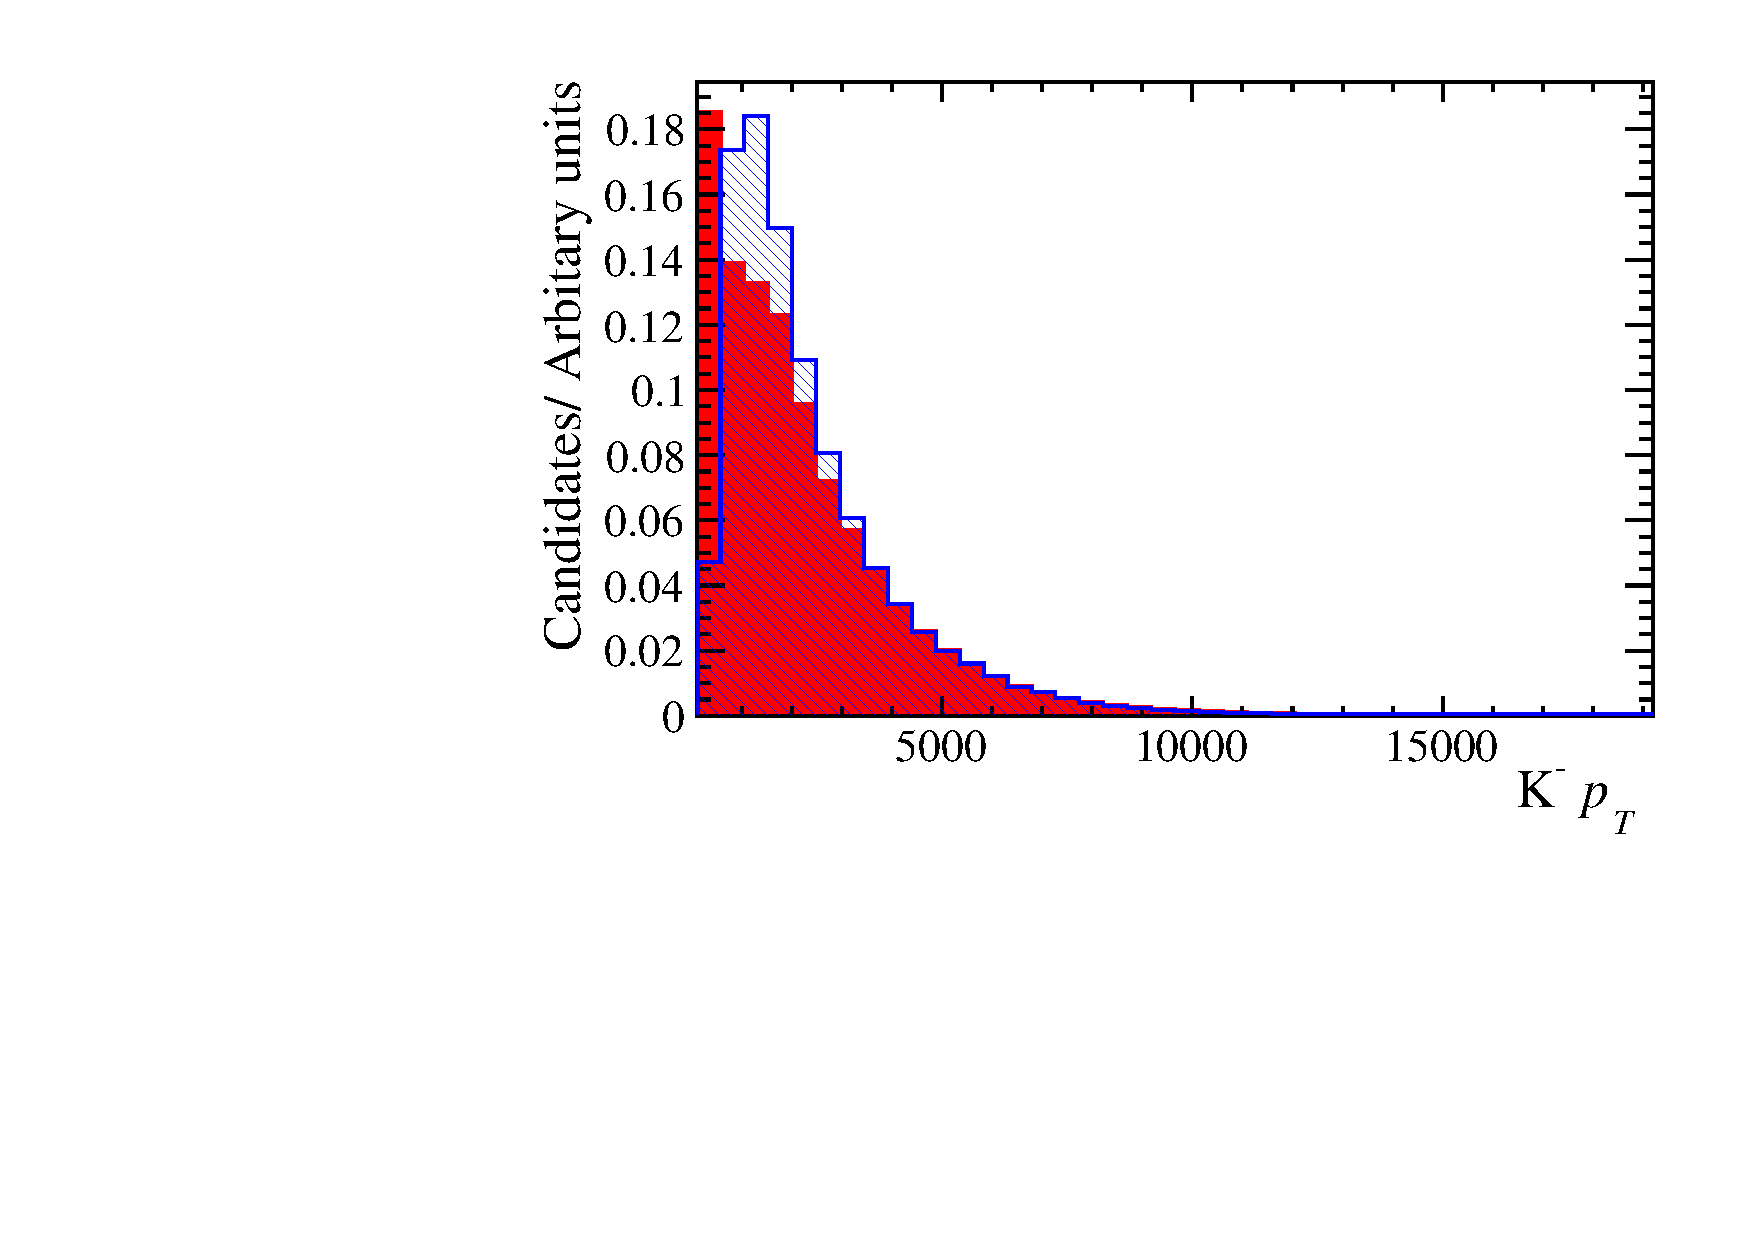
\includegraphics[width=1.0\textwidth]{figs/Selection/Ds_BDT_Var_Ds2KKPi_D_K1_PT.pdf}
   \end{subfigure}
   \begin{subfigure}[t]{0.22\textwidth}
      \centering
      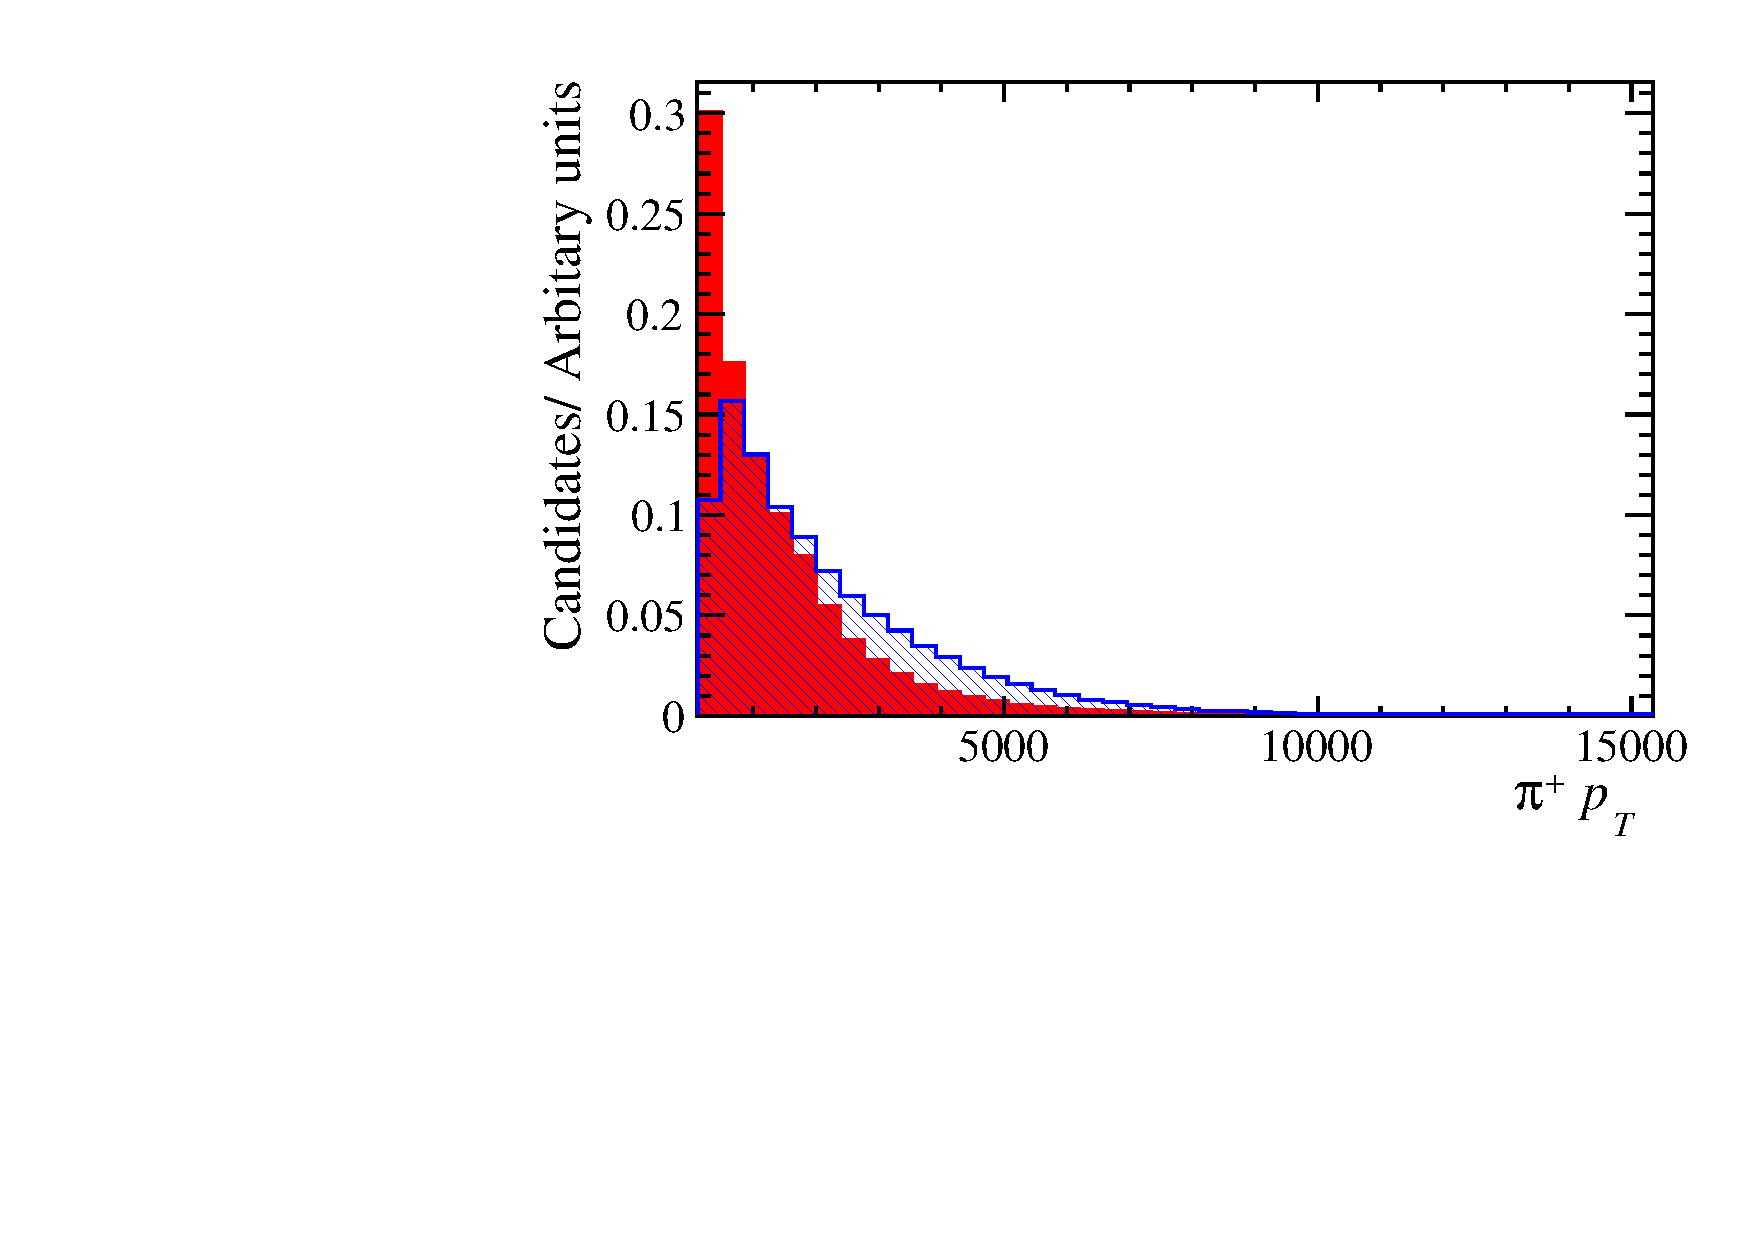
\includegraphics[width=1.0\textwidth]{figs/Selection/Ds_BDT_Var_Ds2KKPi_D_P_PT.pdf}
   \end{subfigure}
   \begin{subfigure}[t]{0.22\textwidth}
      \centering
      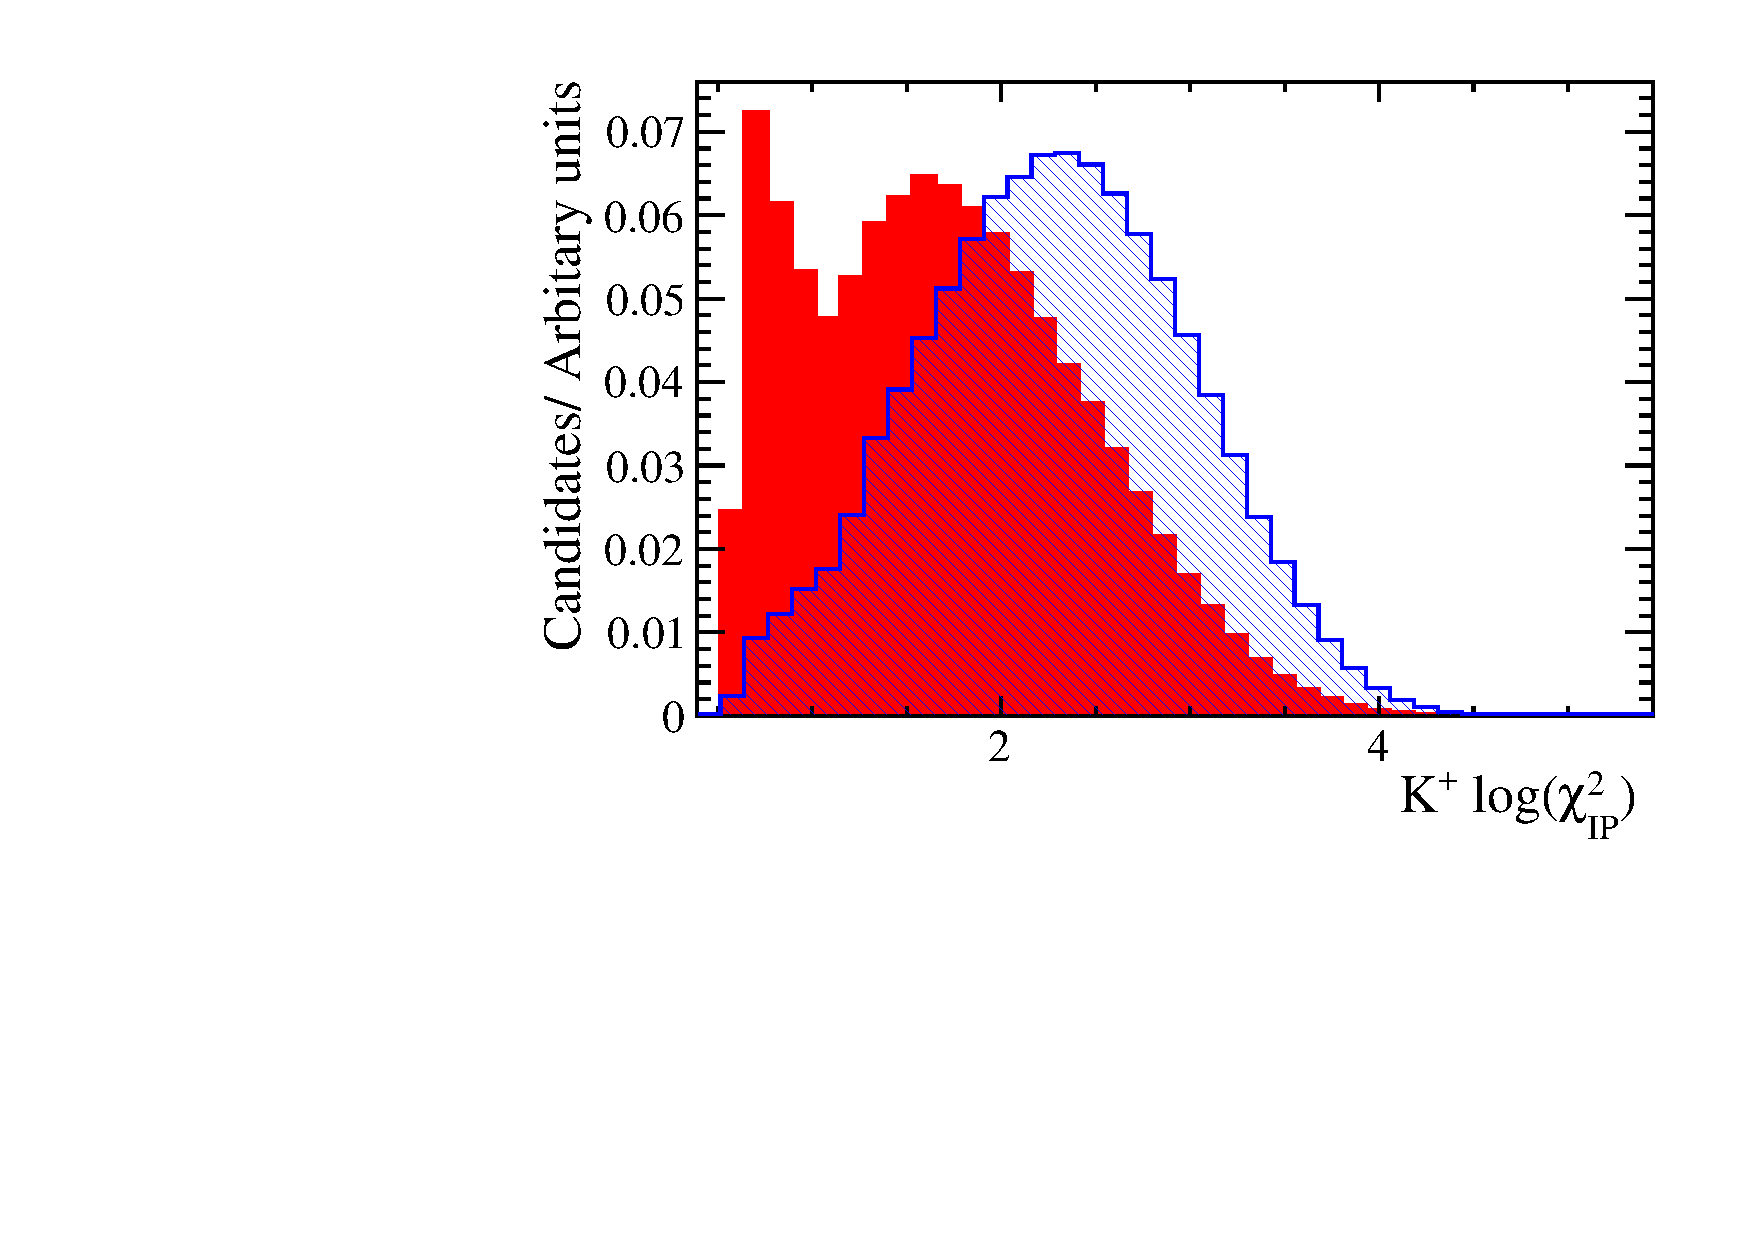
\includegraphics[width=1.0\textwidth]{figs/Selection/Ds_BDT_Var_Ds2KKPi_log10_D_K0_IPCHI2_OWNPV.pdf}
   \end{subfigure}
   \begin{subfigure}[t]{0.22\textwidth}
      \centering
      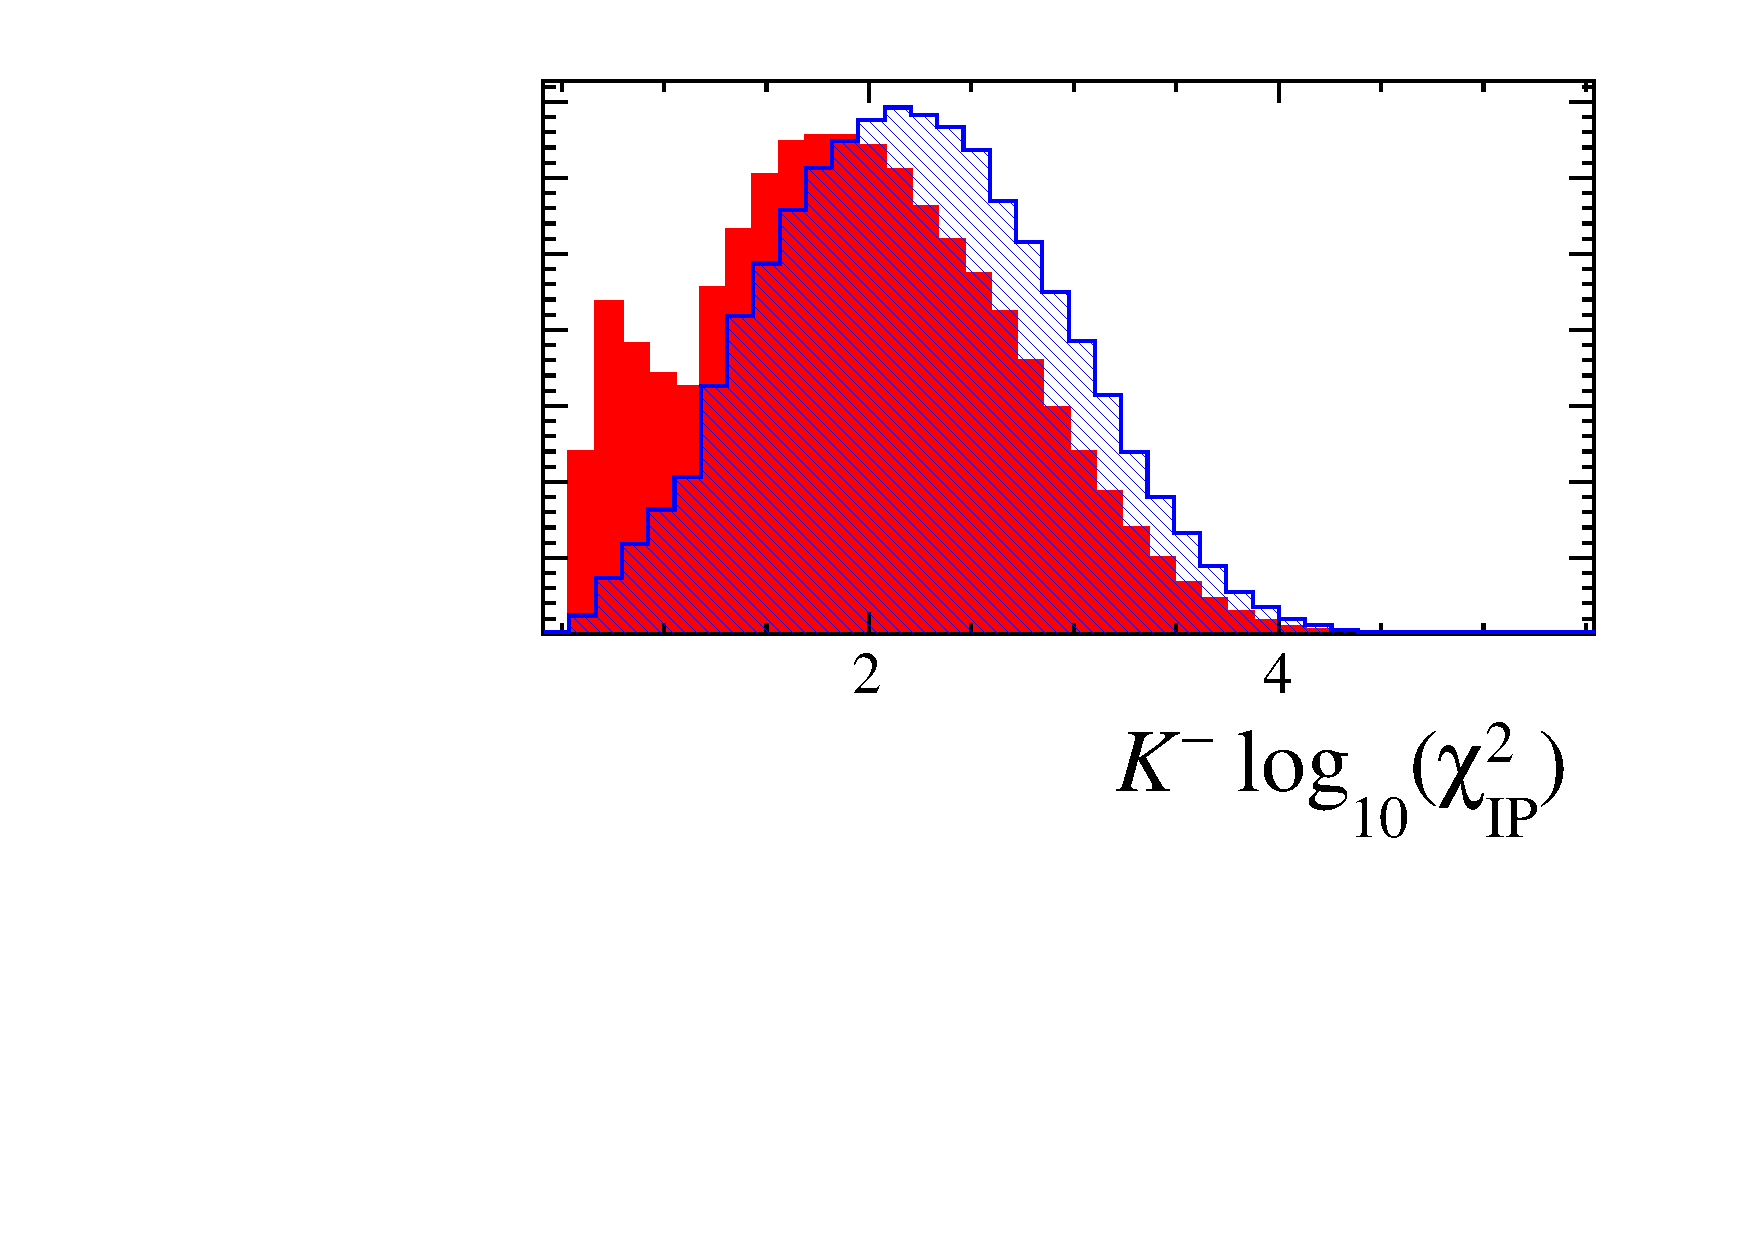
\includegraphics[width=1.0\textwidth]{figs/Selection/Ds_BDT_Var_Ds2KKPi_log10_D_K1_IPCHI2_OWNPV.pdf}
   \end{subfigure}
   \begin{subfigure}[t]{0.22\textwidth}
      \centering
      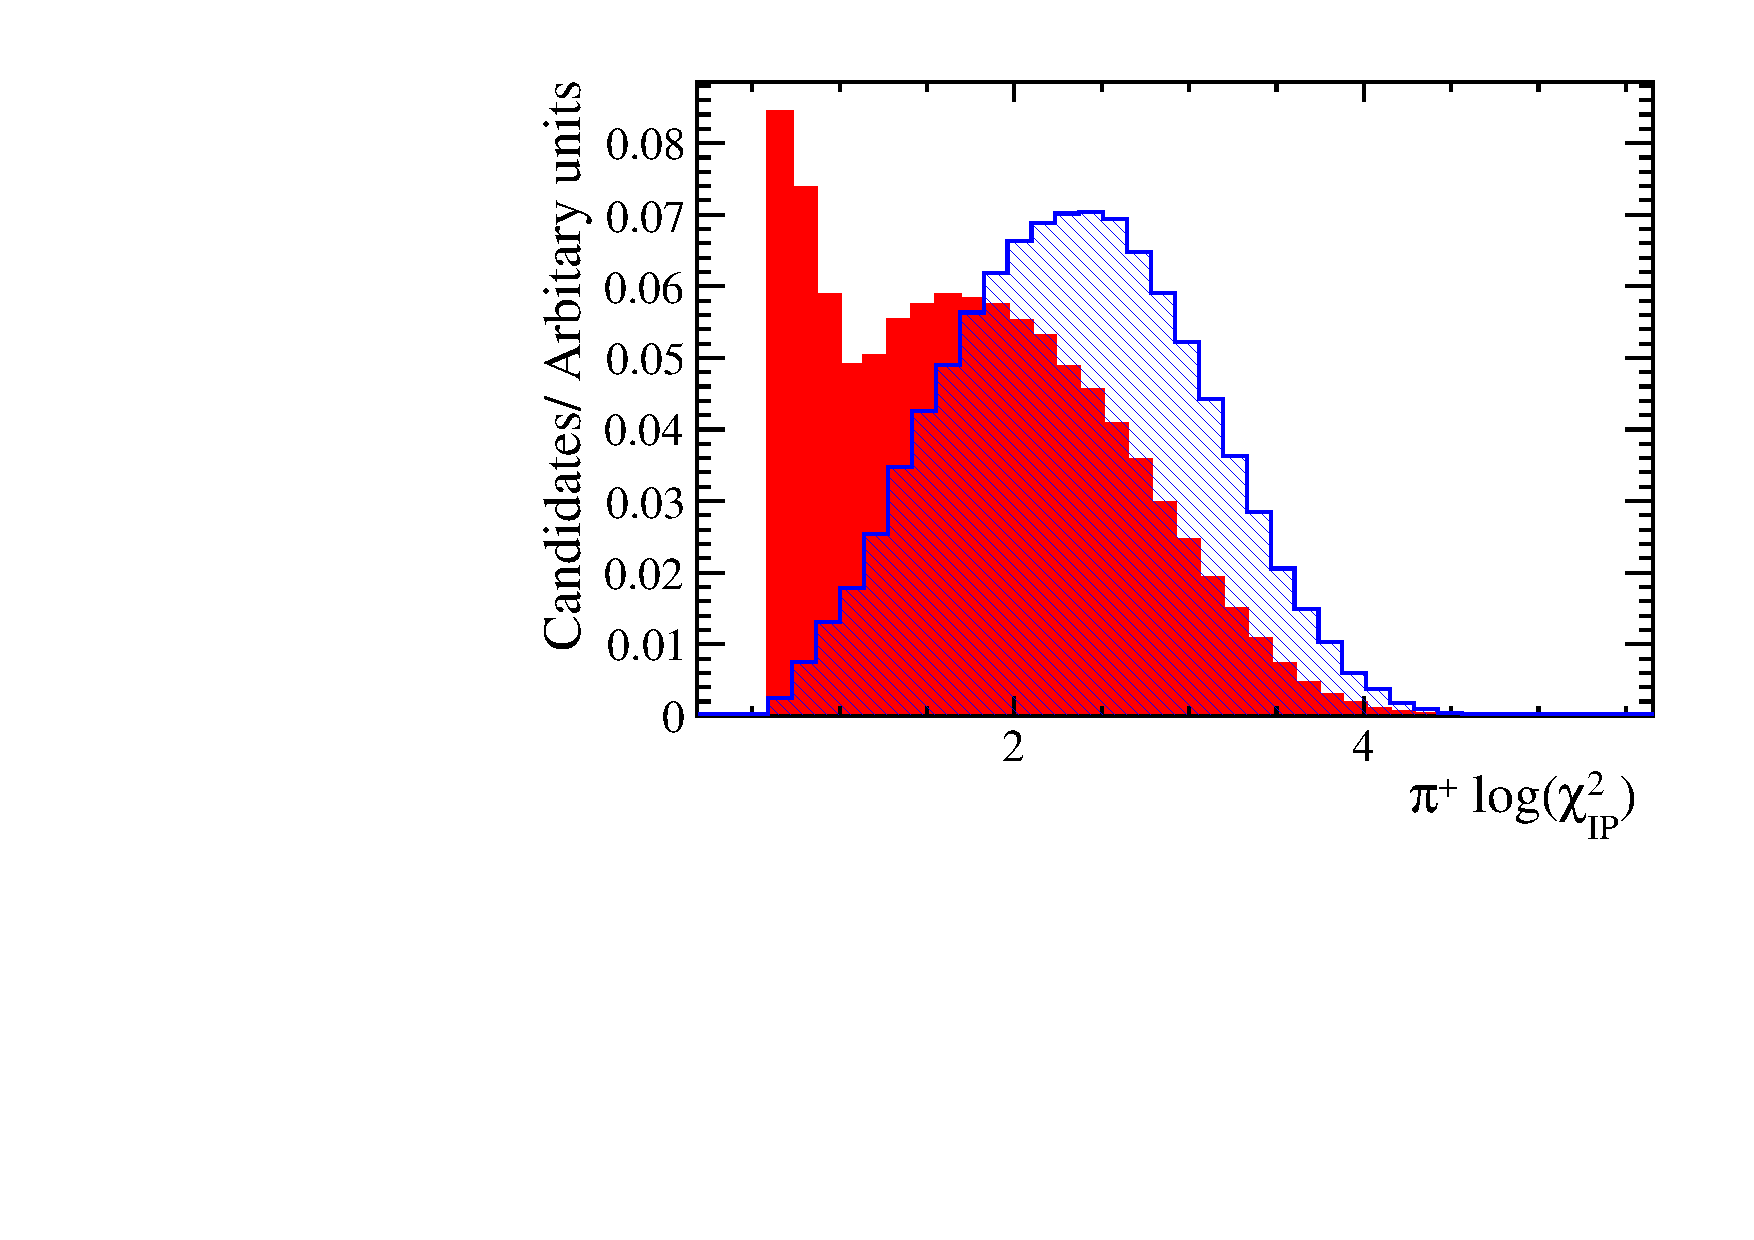
\includegraphics[width=1.0\textwidth]{figs/Selection/Ds_BDT_Var_Ds2KKPi_log10_D_P_IPCHI2_OWNPV.pdf}
   \end{subfigure}
   \begin{subfigure}[t]{0.22\textwidth}
      \centering
      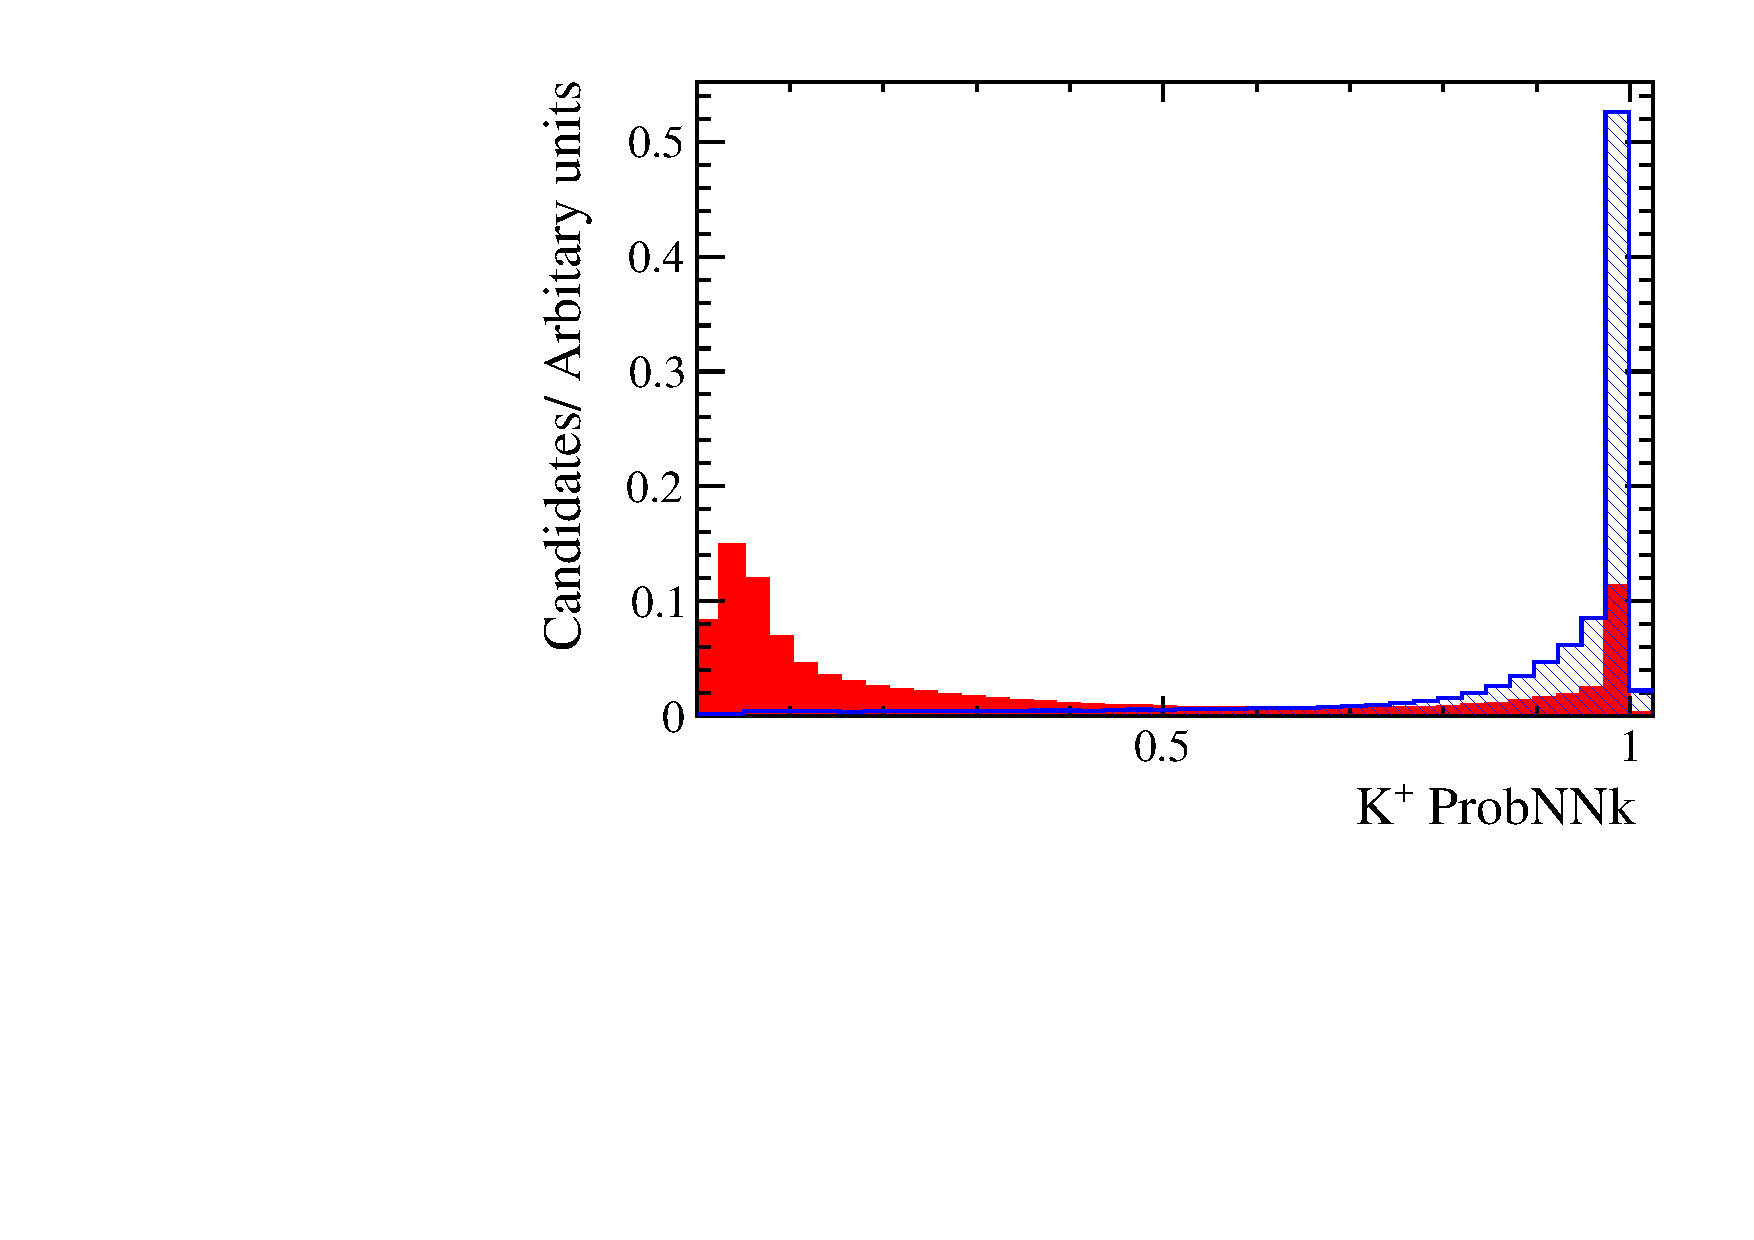
\includegraphics[width=1.0\textwidth]{figs/Selection/Ds_BDT_Var_Ds2KKPi_D_K0_MC15TuneV1_ProbNNk.pdf}
   \end{subfigure}
   \begin{subfigure}[t]{0.22\textwidth}
      \centering
      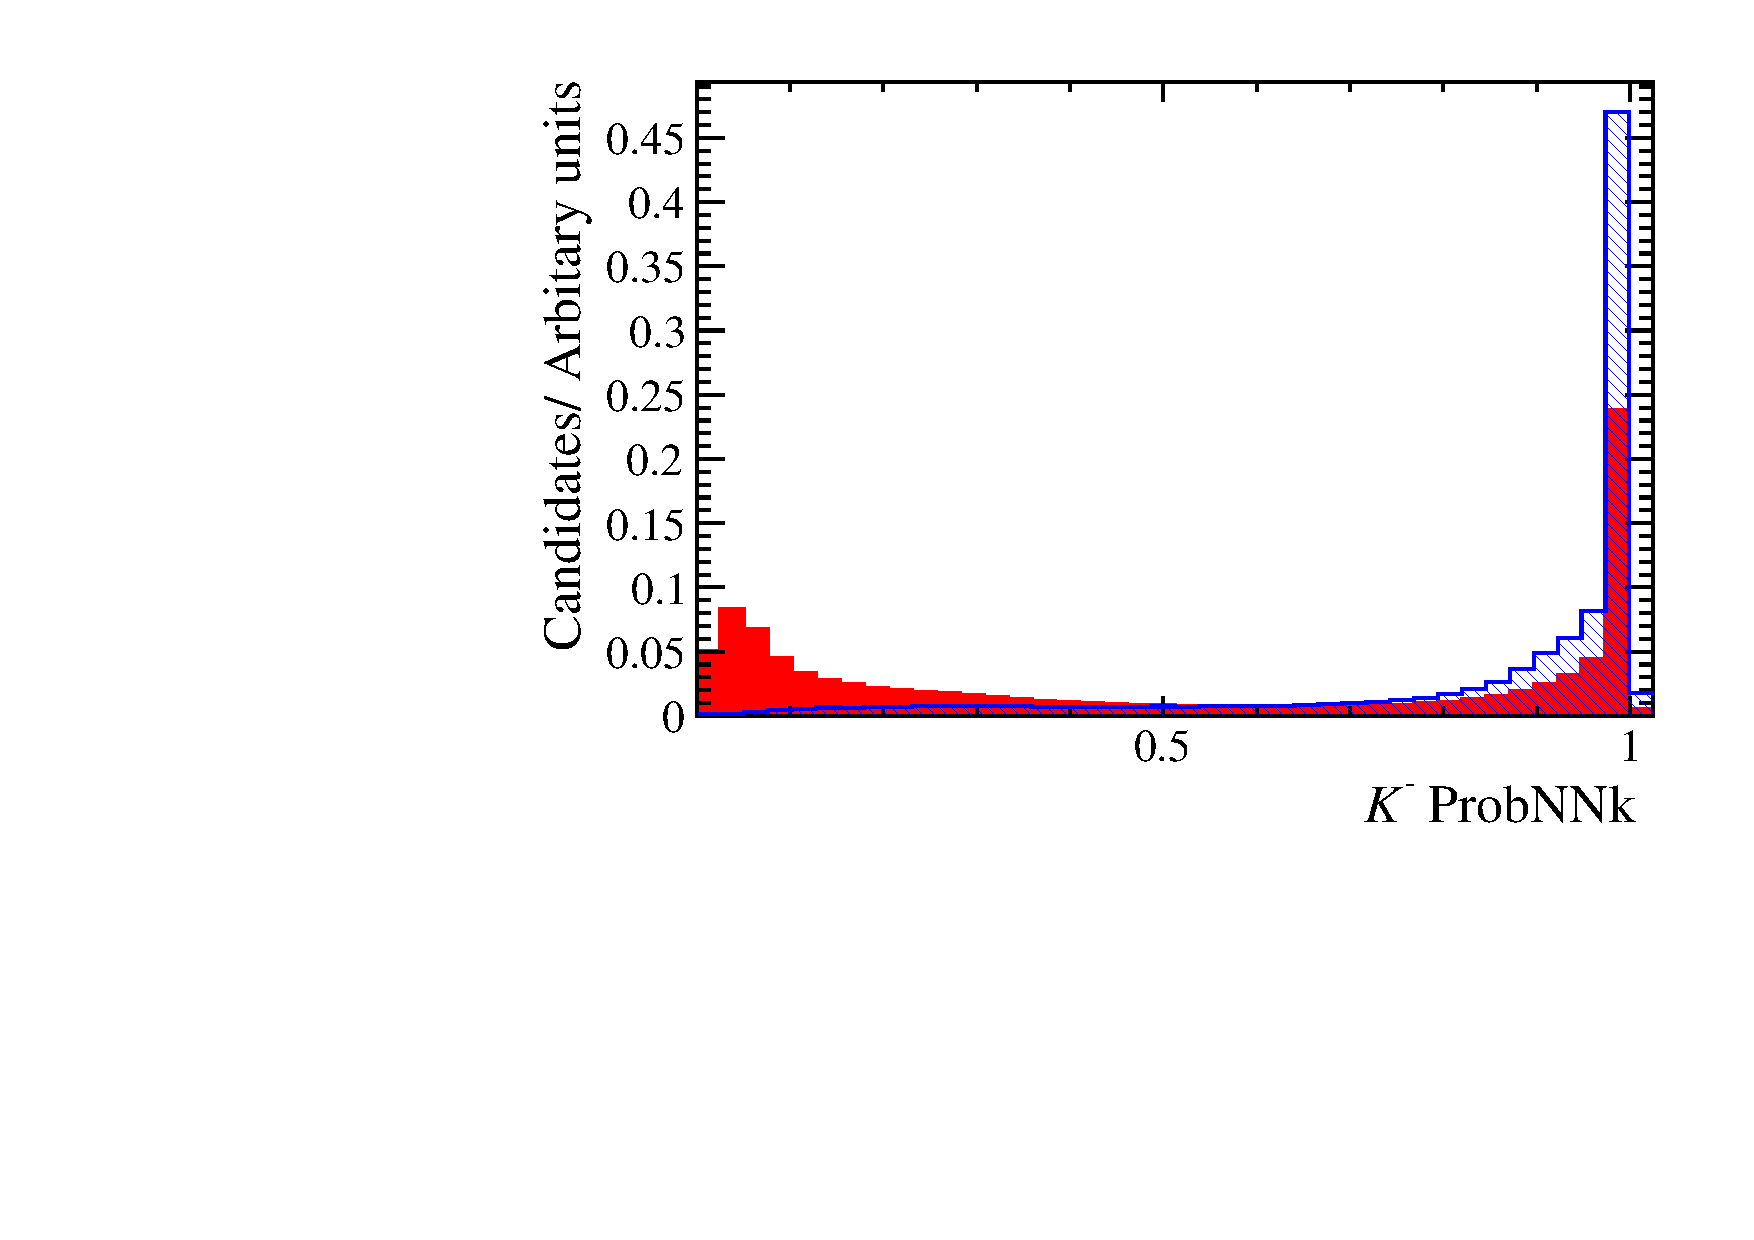
\includegraphics[width=1.0\textwidth]{figs/Selection/Ds_BDT_Var_Ds2KKPi_D_K1_MC15TuneV1_ProbNNk.pdf}
   \end{subfigure}
   \begin{subfigure}[t]{0.22\textwidth}
      \centering
      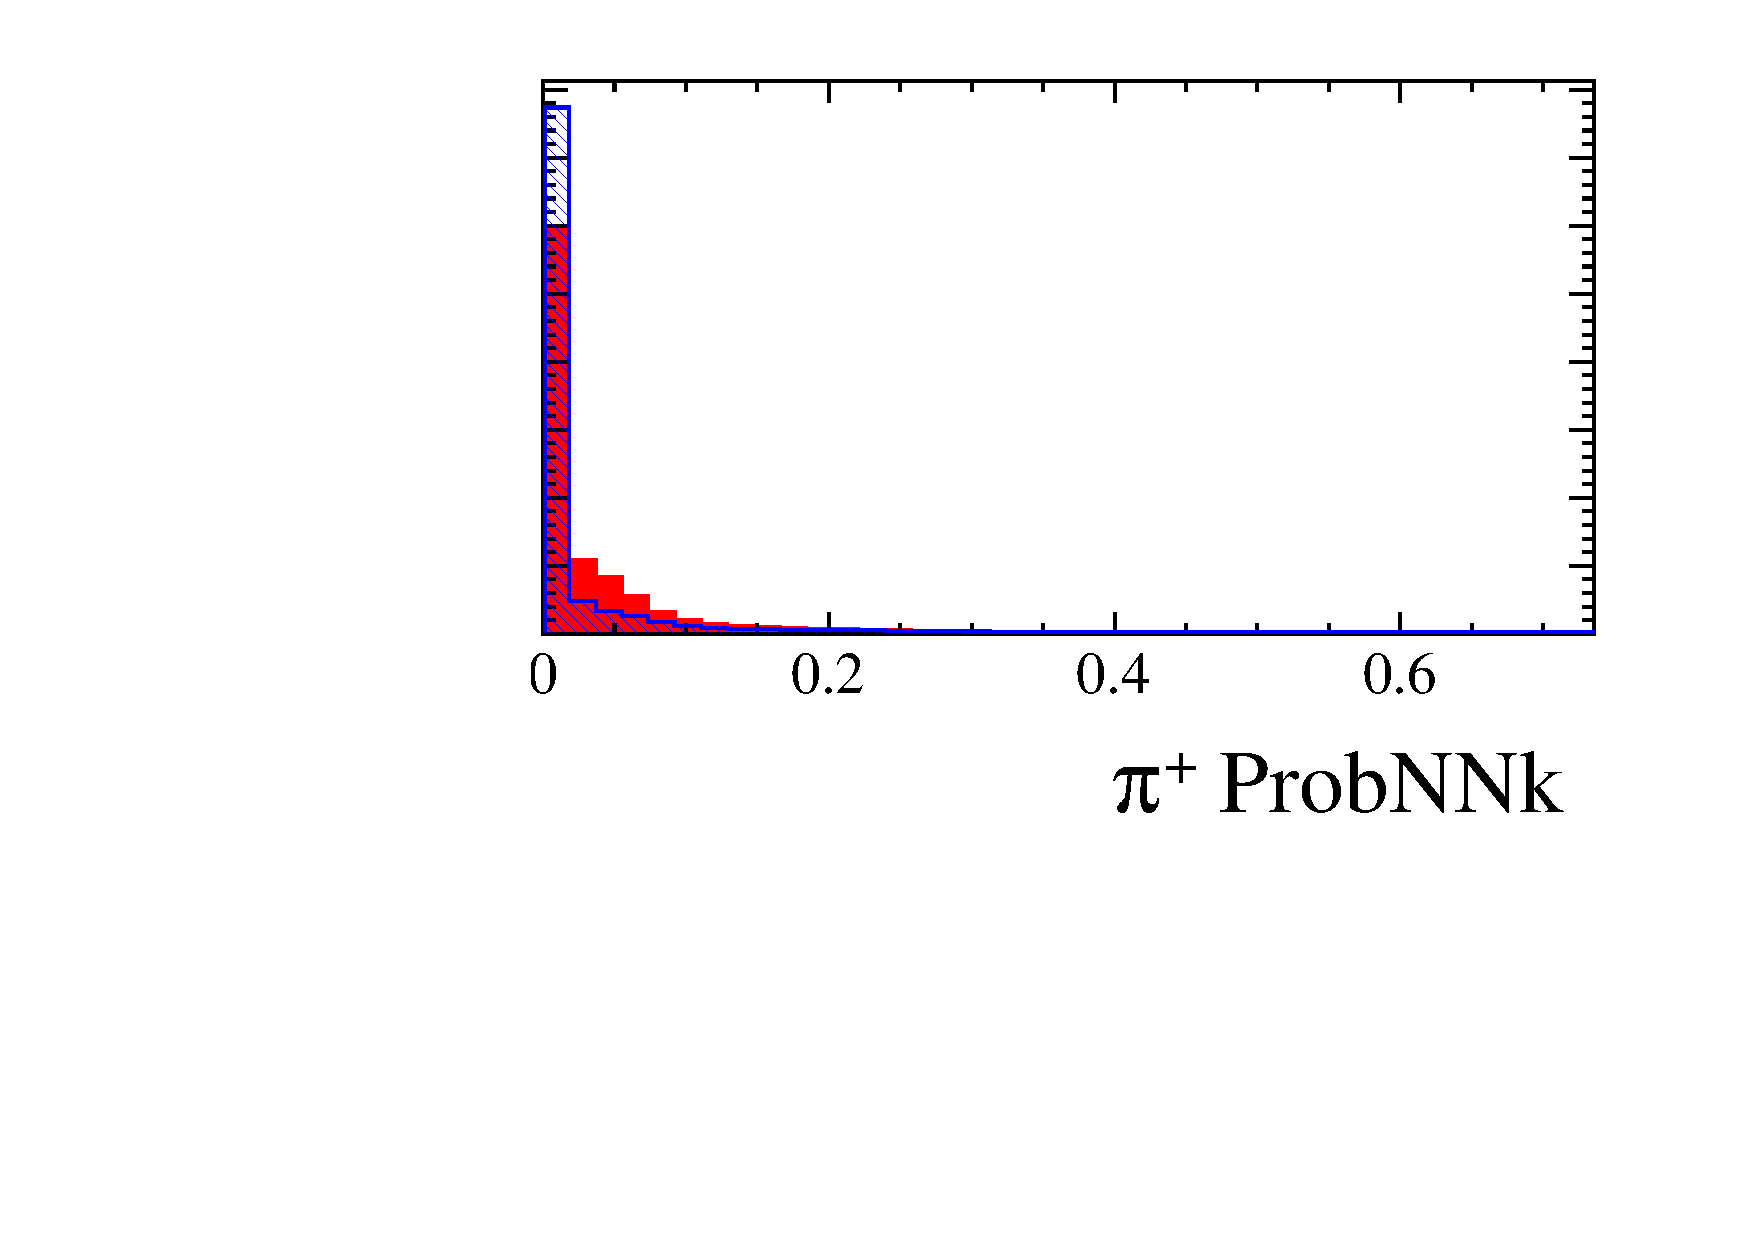
\includegraphics[width=1.0\textwidth]{figs/Selection/Ds_BDT_Var_Ds2KKPi_D_P_MC15TuneV1_ProbNNk.pdf}
   \end{subfigure}
   \begin{subfigure}[t]{0.22\textwidth}
      \centering
      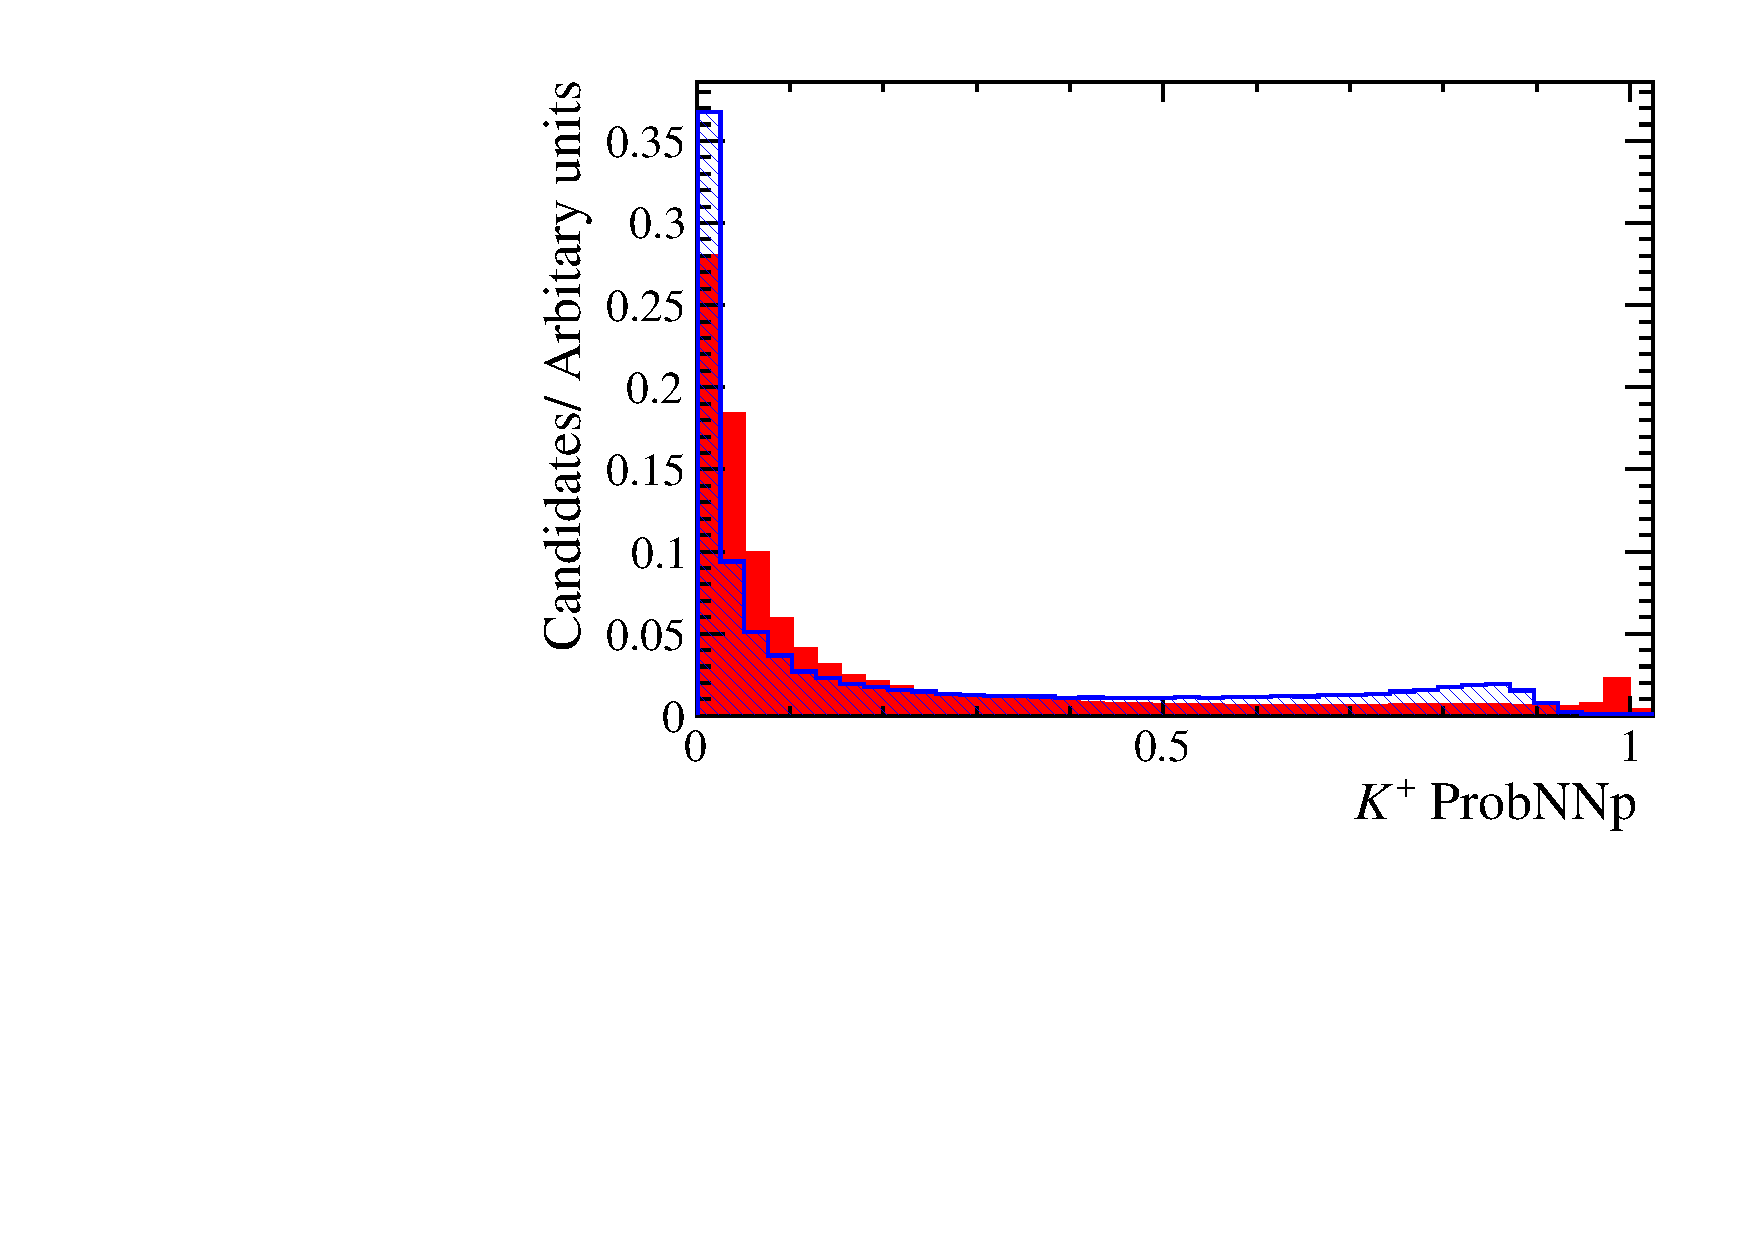
\includegraphics[width=1.0\textwidth]{figs/Selection/Ds_BDT_Var_Ds2KKPi_D_K0_MC15TuneV1_ProbNNp.pdf}
   \end{subfigure}
   \begin{subfigure}[t]{0.22\textwidth}
      \centering
      \includegraphics[width=1.0\textwidth]{figs/Selection/Ds_BDT_Var_Ds2KKPi_D_K1_MC15TuneV1_ProbNNp.pdf}
   \end{subfigure}
   \begin{subfigure}[t]{0.22\textwidth}
      \centering
      \includegraphics[width=1.0\textwidth]{figs/Selection/Ds_BDT_Var_Ds2KKPi_D_P_MC15TuneV1_ProbNNp.pdf}
   \end{subfigure}
   \begin{subfigure}[t]{0.22\textwidth}
      \centering
      \includegraphics[width=1.0\textwidth]{figs/Selection/Ds_BDT_Var_Ds2KKPi_D_K0_MC15TuneV1_ProbNNpi.pdf}
   \end{subfigure}
   \begin{subfigure}[t]{0.22\textwidth}
      \centering
      \includegraphics[width=1.0\textwidth]{figs/Selection/Ds_BDT_Var_Ds2KKPi_D_K1_MC15TuneV1_ProbNNpi.pdf}
   \end{subfigure}
   \begin{subfigure}[t]{0.22\textwidth}
      \centering
      \includegraphics[width=1.0\textwidth]{figs/Selection/Ds_BDT_Var_Ds2KKPi_D_P_MC15TuneV1_ProbNNpi.pdf}
   \end{subfigure}
   \begin{subfigure}[t]{0.22\textwidth}
      \centering
      \includegraphics[width=1.0\textwidth]{figs/Selection/Ds_BDT_Var_Ds2KKPi_D_K0_MC15TuneV1_ProbNNghost.pdf}
   \end{subfigure}
   \begin{subfigure}[t]{0.22\textwidth}
      \centering
      \includegraphics[width=1.0\textwidth]{figs/Selection/Ds_BDT_Var_Ds2KKPi_D_K1_MC15TuneV1_ProbNNghost.pdf}
   \end{subfigure}
   \begin{subfigure}[t]{0.22\textwidth}
      \centering
      \includegraphics[width=1.0\textwidth]{figs/Selection/Ds_BDT_Var_Ds2KKPi_D_P_MC15TuneV1_ProbNNghost.pdf}
   \end{subfigure}
   \begin{subfigure}[t]{0.22\textwidth}
      \centering
      \includegraphics[width=1.0\textwidth]{figs/Selection/Ds_BDT_Var_Ds2KKPi_D_K0_BDT_TRACK_VeloCHI2NDOF.pdf}
   \end{subfigure}
   \begin{subfigure}[t]{0.22\textwidth}
      \centering
      \includegraphics[width=1.0\textwidth]{figs/Selection/Ds_BDT_Var_Ds2KKPi_D_K1_BDT_TRACK_VeloCHI2NDOF.pdf}
   \end{subfigure}
   \begin{subfigure}[t]{0.22\textwidth}
      \centering
      \includegraphics[width=1.0\textwidth]{figs/Selection/Ds_BDT_Var_Ds2KKPi_D_P_BDT_TRACK_VeloCHI2NDOF.pdf}
   \end{subfigure}
   \begin{subfigure}[t]{0.22\textwidth}
      \centering
      \includegraphics[width=1.0\textwidth]{figs/Selection/Ds_BDT_Var_Ds2KKPi_D_K0_TRACK_CHI2NDOF.pdf}
   \end{subfigure}
   \begin{subfigure}[t]{0.22\textwidth}
      \centering
      \includegraphics[width=1.0\textwidth]{figs/Selection/Ds_BDT_Var_Ds2KKPi_D_K1_TRACK_CHI2NDOF.pdf}
   \end{subfigure}
   \begin{subfigure}[t]{0.22\textwidth}
      \centering
      \includegraphics[width=1.0\textwidth]{figs/Selection/Ds_BDT_Var_Ds2KKPi_D_P_TRACK_CHI2NDOF.pdf}
   \end{subfigure}
   \begin{subfigure}[t]{0.22\textwidth}
      \centering
      \includegraphics[width=1.0\textwidth]{figs/Selection/Ds_BDT_Var_Ds2KKPi_D_K0_TRACK_MatchCHI2.pdf}
   \end{subfigure}
   \begin{subfigure}[t]{0.22\textwidth}
      \centering
      \includegraphics[width=1.0\textwidth]{figs/Selection/Ds_BDT_Var_Ds2KKPi_D_K1_TRACK_MatchCHI2.pdf}
   \end{subfigure}
   \begin{subfigure}[t]{0.22\textwidth}
      \centering
      \includegraphics[width=1.0\textwidth]{figs/Selection/Ds_BDT_Var_Ds2KKPi_D_P_TRACK_MatchCHI2.pdf}
   \end{subfigure}
   \caption{Distributions of MVA training variables in the signal (blue) and background (red) samples for the Run~II \decay{\Dsp}{\Kp\Km\pip} MVA.}
   \label{fig:mvatrainingvariables_Ds}   
\end{figure}
%%%%%%%%%%%%%%%%%%%%%%%%%%%%%%%%%%%%%%%%%%%%%%%%%%%%%%%%%%

\clearpage
\section{MVA method}
\label{sec:app_mva_method}


In this data-driven MVA approach, the `signal' and `background' training samples are both taken from the relevant \decay{\Bsb}{\Dsp\pim} or \decay{\Bs}{\jpsi\phiz} decay samples.
The signal samples include all events within the background subtraction fit ranges. Each candidate is weighted with the appropriate Gaussian fit component weight as determined by the \sPlot technique. This weight is passed to the \tmva framework when training the methods.
The background samples are comprised of the sideband regions of the relevant ranges in Fig.~\ref{fig:mvatrainingsamples}. These ranges are defined by $|m(\Kp\Km)-m(\phiz)| > 10 \mevcc$ and $|m(h^{+}h^{-}h^{+})-m(\Dsp)| > 30\mevcc$ for the \phiz and \Dsp MVAs respectively. No weights are used for the background samples as the regions are known to be signal-deficient.



The MVAs are trained using Gradient Boosted Decision Trees (BDTGs)~\cite{Breiman}. This method was compared to a number of different Boosted Decision Tree (BDT) derivatives and found to be most effective.

The BDTG method categorises `signal' and `background' candidates by creating consecutive sets of questions called Decision Trees. Each question can have two possible answers and depends on the previous responses. Eventually the answer to a question results in a candidate being classes as `signal' or `background' rather than asking more questions. A definable number of decision trees are used to collectively categorise each candidate; the overall response combines the decisions of all trees. The trees are trained using \emph{boosting}. This means candidates that are most likely to be misclassified are weighted higher, such that the later trees concentrate on these trickier areas.  
The boosting method utilised in the BDTG method is designed to be more robust and reproducible in noisy situations, for example with limited statistics. 
The BDTG method is used in training all MVAs.


%%%%%%%%%%%%%%%%%%%%%%%%%%%%%%%%%%%%%%%%%%%%%%%%%%%%%%%%%%
\begin{figure}[!h]
   \centering
   \begin{subfigure}[t]{0.32\textwidth}
      \centering
      \includegraphics[width=1.0\textwidth]{figs/Selection/Phi_BDT_classifier_Run1.pdf}
      \caption{Run I \decay{\phiz}{\Kp\Km}}
   \end{subfigure}
   \begin{subfigure}[t]{0.32\textwidth}
      \centering
      \includegraphics[width=1.0\textwidth]{figs/Selection/Phi_BDT_classifier_Run2.pdf}
      \caption{Run II \decay{\phiz}{\Kp\Km}}
   \end{subfigure}\\
   \begin{subfigure}[t]{0.32\textwidth}
      \centering
      \includegraphics[width=1.0\textwidth]{figs/Selection/Ds_BDT_classifier_Ds2KKPi_Run1.pdf}
      \caption{Run I \decay{\Dsp}{\Kp\Km\pip}}
   \end{subfigure}
   \begin{subfigure}[t]{0.32\textwidth}
      \centering
      \includegraphics[width=1.0\textwidth]{figs/Selection/Ds_BDT_classifier_Ds2KKPi_Run2.pdf}
      \caption{Run II \decay{\Dsp}{\Kp\Km\pip}}
   \end{subfigure}\\
   \begin{subfigure}[t]{0.32\textwidth}
      \centering
      \includegraphics[width=1.0\textwidth]{figs/Selection/Ds_BDT_classifier_Ds2PiPiPi_Run1.pdf}
      \caption{Run I \decay{\Dsp}{\pip\pim\pip}}
   \end{subfigure}
   \begin{subfigure}[t]{0.32\textwidth}
      \centering
      \includegraphics[width=1.0\textwidth]{figs/Selection/Ds_BDT_classifier_Ds2PiPiPi_Run2.pdf}
      \caption{Run II \decay{\Dsp}{\pip\pim\pip}}
   \end{subfigure}\\
   \begin{subfigure}[t]{0.32\textwidth}
      \centering
      \includegraphics[width=1.0\textwidth]{figs/Selection/Ds_BDT_classifier_Ds2KPiPi_Run1.pdf}
      \caption{Run I \decay{\Dsp}{\Kp\pim\pip}}
   \end{subfigure}
   \begin{subfigure}[t]{0.32\textwidth}
      \centering
      \includegraphics[width=1.0\textwidth]{figs/Selection/Ds_BDT_classifier_Ds2KPiPi_Run2.pdf}
      \caption{Run II \decay{\Dsp}{\Kp\pim\pip}}
   \end{subfigure}\\
   \caption{MVA classifier response for the eight MVAs trained for both signal (blue) and background (red). The training samples are represented by markers and the validation samples by filled histograms.}
   \label{fig:mvaclassifierresponses}   
\end{figure}
%%%%%%%%%%%%%%%%%%%%%%%%%%%%%%%%%%%%%%%%%%%%%%%%%%%%%%%%%%

The MVA classifier distributions for each of the eight MVAs trained are shown in Fig.~\ref{fig:mvaclassifierresponses}. This figure shows both the signal and background samples, as well as the training and validation subsamples. Each mode shows a good separation between the signal and background samples. For the majority of the distributions the training and testing samples have almost identical shapes, implying response is reproducible and the method has not overtrained. There are noticeable exceptions, however. The signal training and validation samples tend to show different distributions in the regions where the background distributions are maximal. This effect is likely to be a result of the use of weights in the MVA training. Ideally, the MVA classifier should remain positive across the whole range. The negative values implies that in that range the MVA classifier is correlated to the parameter used to generate the weights: the \phiz or \Dsp mass. As this only affects the range of MVA classifier values that are dominantly `background'-like, it likely this discrepancy is due specifically to presence of weighted background events in the signal sample passed to \tmva.
This effect is further studied to determine if it results in any systematic uncertainty in the MVA efficiencies as discussed in Sections~\ref{sec:B2DsKK_systuncertainy} and~\ref{sec:B2DsPhi_systuncertainy}. In all cases the discrepancies are far below the range of values that selection requirements are placed. 

\section{Optimisation}
\label{sec:app_mva_optimisation}
The VA optimisation is performed in two dimensions, one for each of the \phiz and \Dsp MVAs. This is performed separately for the three different \Dsp decay modes. The results of the optimisation for each \Dsp decay mode and running period are shown in Fig.~\ref{fig:mvaoptmisation}. 
%%%%%%%%%%%%%%%%%%%%%%%%%%%%%%%%%%%%%%%%%%%%%%%%%%%%%%%%%%
\begin{figure}[!h]
   \centering
   \begin{subfigure}[t]{0.4\textwidth}
      \centering
      \includegraphics[width=1.0\textwidth]{figs/Selection/Ds2KKPi_BDTG_punzi_Run1_cont.pdf}
      \caption{Run I \decay{\Dsp}{\Kp\Km\pip}}
   \end{subfigure}
   \begin{subfigure}[t]{0.4\textwidth}
      \centering
      \includegraphics[width=1.0\textwidth]{figs/Selection/Ds2KKPi_BDTG_punzi_Run2_cont.pdf}
      \caption{Run II \decay{\Dsp}{\Kp\Km\pip}}
   \end{subfigure}\\
   \begin{subfigure}[t]{0.4\textwidth}
      \centering
      \includegraphics[width=1.0\textwidth]{figs/Selection/Ds2PiPiPi_BDTG_punzi_Run1_cont.pdf}
      \caption{Run I \decay{\Dsp}{\pip\pim\pip}}
   \end{subfigure}
   \begin{subfigure}[t]{0.4\textwidth}
      \centering
      \includegraphics[width=1.0\textwidth]{figs/Selection/Ds2PiPiPi_BDTG_punzi_Run2_cont.pdf}
      \caption{Run II \decay{\Dsp}{\pip\pim\pip}}
   \end{subfigure}\\
   \begin{subfigure}[t]{0.4\textwidth}
      \centering
      \includegraphics[width=1.0\textwidth]{figs/Selection/Ds2KPiPi_BDTG_punzi_Run1_cont.pdf}
      \caption{Run I \decay{\Dsp}{\Kp\pim\pip}}
   \end{subfigure}
   \begin{subfigure}[t]{0.4\textwidth}
      \centering
      \includegraphics[width=1.0\textwidth]{figs/Selection/Ds2KPiPi_BDTG_punzi_Run2_cont.pdf}
      \caption{Run II \decay{\Dsp}{\Kp\pim\pip}}
   \end{subfigure}\\
   \caption{FOM versus MVA requirements.}
   \label{fig:mvaoptmisation}   
\end{figure}
%%%%%%%%%%%%%%%%%%%%%%%%%%%%%%%%%%%%%%%%%%%%%%%%%%%%%%%%%%

The optimal values are selected separately for each of the modes and tabulated in Table~\ref{table:mvarequirementvalues}.

\begin{table}[!h]
\centering
\begin{tabular}{ l l  c  c  }

\hline
Period   & \Dsp decay mode               & \Dsp requirement & \phiz/\Dzb requirement \\ 
\hline
Run I    & \decay{\Dsp}{\Kp\Km\pip}      & 0.5 & 0.8 \\
         & \decay{\Dsp}{\pip\pim\pip}    & 0.3 & 0.8 \\
         & \decay{\Dsp}{\Kp\pim\pip}     & 0.2 & 0.8 \\ 
\hline
Run II   & \decay{\Dsp}{\Kp\Km\pip}      & 0.5 & 0.8 \\
         & \decay{\Dsp}{\pip\pim\pip}    & 0.2 & 0.8 \\
         & \decay{\Dsp}{\Kp\pim\pip}     & 0.2 & 0.8 \\                                      
\hline
\end{tabular}
\caption{Optimised MVA cuts for the different \Dsp decay modes and datasets. }
\label{table:mvarequirementvalues}

\end{table}
